\documentclass[twoside]{book}

% Packages required by doxygen
\usepackage{fixltx2e}
\usepackage{calc}
\usepackage{doxygen}
\usepackage[export]{adjustbox} % also loads graphicx
\usepackage{graphicx}
\usepackage[utf8]{inputenc}
\usepackage{makeidx}
\usepackage{multicol}
\usepackage{multirow}
\PassOptionsToPackage{warn}{textcomp}
\usepackage{textcomp}
\usepackage[nointegrals]{wasysym}
\usepackage[table]{xcolor}

% Font selection
\usepackage[T1]{fontenc}
\usepackage[scaled=.90]{helvet}
\usepackage{courier}
\usepackage{amssymb}
\usepackage{sectsty}
\renewcommand{\familydefault}{\sfdefault}
\allsectionsfont{%
  \fontseries{bc}\selectfont%
  \color{darkgray}%
}
\renewcommand{\DoxyLabelFont}{%
  \fontseries{bc}\selectfont%
  \color{darkgray}%
}
\newcommand{\+}{\discretionary{\mbox{\scriptsize$\hookleftarrow$}}{}{}}

% Page & text layout
\usepackage{geometry}
\geometry{%
  a4paper,%
  top=2.5cm,%
  bottom=2.5cm,%
  left=2.5cm,%
  right=2.5cm%
}
\tolerance=750
\hfuzz=15pt
\hbadness=750
\setlength{\emergencystretch}{15pt}
\setlength{\parindent}{0cm}
\setlength{\parskip}{3ex plus 2ex minus 2ex}
\makeatletter
\renewcommand{\paragraph}{%
  \@startsection{paragraph}{4}{0ex}{-1.0ex}{1.0ex}{%
    \normalfont\normalsize\bfseries\SS@parafont%
  }%
}
\renewcommand{\subparagraph}{%
  \@startsection{subparagraph}{5}{0ex}{-1.0ex}{1.0ex}{%
    \normalfont\normalsize\bfseries\SS@subparafont%
  }%
}
\makeatother

% Headers & footers
\usepackage{fancyhdr}
\pagestyle{fancyplain}
\fancyhead[LE]{\fancyplain{}{\bfseries\thepage}}
\fancyhead[CE]{\fancyplain{}{}}
\fancyhead[RE]{\fancyplain{}{\bfseries\leftmark}}
\fancyhead[LO]{\fancyplain{}{\bfseries\rightmark}}
\fancyhead[CO]{\fancyplain{}{}}
\fancyhead[RO]{\fancyplain{}{\bfseries\thepage}}
\fancyfoot[LE]{\fancyplain{}{}}
\fancyfoot[CE]{\fancyplain{}{}}
\fancyfoot[RE]{\fancyplain{}{\bfseries\scriptsize Generated by Doxygen }}
\fancyfoot[LO]{\fancyplain{}{\bfseries\scriptsize Generated by Doxygen }}
\fancyfoot[CO]{\fancyplain{}{}}
\fancyfoot[RO]{\fancyplain{}{}}
\renewcommand{\footrulewidth}{0.4pt}
\renewcommand{\chaptermark}[1]{%
  \markboth{#1}{}%
}
\renewcommand{\sectionmark}[1]{%
  \markright{\thesection\ #1}%
}

% Indices & bibliography
\usepackage{natbib}
\usepackage[titles]{tocloft}
\setcounter{tocdepth}{3}
\setcounter{secnumdepth}{5}
\makeindex

% Hyperlinks (required, but should be loaded last)
\usepackage{ifpdf}
\ifpdf
  \usepackage[pdftex,pagebackref=true]{hyperref}
\else
  \usepackage[ps2pdf,pagebackref=true]{hyperref}
\fi
\hypersetup{%
  colorlinks=true,%
  linkcolor=blue,%
  citecolor=blue,%
  unicode%
}

% Custom commands
\newcommand{\clearemptydoublepage}{%
  \newpage{\pagestyle{empty}\cleardoublepage}%
}

\usepackage{caption}
\captionsetup{labelsep=space,justification=centering,font={bf},singlelinecheck=off,skip=4pt,position=top}

%===== C O N T E N T S =====

\begin{document}

% Titlepage & ToC
\hypersetup{pageanchor=false,
             bookmarksnumbered=true,
             pdfencoding=unicode
            }
\pagenumbering{alph}
\begin{titlepage}
\vspace*{7cm}
\begin{center}%
{\Large Poynt-\/i\+O\+S-\/\+S\+DK \\[1ex]\large 0.\+1 }\\
\vspace*{1cm}
{\large Generated by Doxygen 1.8.12}\\
\end{center}
\end{titlepage}
\clearemptydoublepage
\pagenumbering{roman}
\tableofcontents
\clearemptydoublepage
\pagenumbering{arabic}
\hypersetup{pageanchor=true}

%--- Begin generated contents ---
\chapter{Poynt i\+O\+S-\/\+S\+DK}
\label{index}\hypertarget{index}{}\hypertarget{index_intro_sec}{}\section{Introduction}\label{index_intro_sec}
The i\+OS S\+DK offers developers a library by which on can communicate directly with a Poynt Smart Terminal using an i\+OS compatible device. Currently the S\+DK supports systems running $>$= i\+OS 8. 
\chapter{Todo List}
\label{todo}
\hypertarget{todo}{}

\begin{DoxyRefList}
\item[\label{todo__todo000001}%
\hypertarget{todo__todo000001}{}%
Class \hyperlink{interface_poynt_terminal}{Poynt\+Terminal} ]allow multiple terminal connections. Currently, only one terminal connection is supported  
\item[\label{todo__todo000002}%
\hypertarget{todo__todo000002}{}%
Global \hyperlink{interface_poynt_transaction_object_ab4cac3360e86d21570d89915c99e6943}{Poynt\+Transaction\+Object\+:\+:funding\+Source} ]at current, we are not populating this field. Developers have access to the data in \hyperlink{interface_poynt_transaction_response_object_a0046f618ca04fd1e7fcf91b87190a944}{Poynt\+Transaction\+Response\+Object.\+raw\+Json} propety 
\end{DoxyRefList}
\chapter{Hierarchical Index}
\section{Class Hierarchy}
This inheritance list is sorted roughly, but not completely, alphabetically\+:\begin{DoxyCompactList}
\item N\+S\+Object\begin{DoxyCompactList}
\item \contentsline{section}{Poynt\+Debug}{\pageref{interface_poynt_debug}}{}
\item \contentsline{section}{Poynt\+Discount\+Object}{\pageref{interface_poynt_discount_object}}{}
\item \contentsline{section}{Poynt\+Order\+Item\+Object}{\pageref{interface_poynt_order_item_object}}{}
\item \contentsline{section}{Poynt\+Order\+Item\+Tax}{\pageref{interface_poynt_order_item_tax}}{}
\item \contentsline{section}{Poynt\+Order\+Object}{\pageref{interface_poynt_order_object}}{}
\item \contentsline{section}{Poynt\+Payment\+Amount\+Object}{\pageref{interface_poynt_payment_amount_object}}{}
\item \contentsline{section}{Poynt\+Payment\+Object}{\pageref{interface_poynt_payment_object}}{}
\item \contentsline{section}{Poynt\+P\+O\+S\+Connection\+Manager}{\pageref{interface_poynt_p_o_s_connection_manager}}{}
\item \contentsline{section}{Poynt\+Terminal}{\pageref{interface_poynt_terminal}}{}
\item \contentsline{section}{Poynt\+Terminal\+Discover}{\pageref{interface_poynt_terminal_discover}}{}
\item \contentsline{section}{Poynt\+Transaction\+Amounts}{\pageref{interface_poynt_transaction_amounts}}{}
\item \contentsline{section}{Poynt\+Transaction\+Object}{\pageref{interface_poynt_transaction_object}}{}
\item \contentsline{section}{Poynt\+Transaction\+Response\+Object}{\pageref{interface_poynt_transaction_response_object}}{}
\end{DoxyCompactList}
\item $<$N\+S\+Object$>$\begin{DoxyCompactList}
\item \contentsline{section}{$<$Poynt\+Transaction $>$}{\pageref{protocol_poynt_transaction_01-p}}{}
\end{DoxyCompactList}
\item $<$Poynt\+Serialized\+Object$>$\begin{DoxyCompactList}
\item \contentsline{section}{Poynt\+Discount\+Object}{\pageref{interface_poynt_discount_object}}{}
\item \contentsline{section}{Poynt\+Order\+Item\+Object}{\pageref{interface_poynt_order_item_object}}{}
\item \contentsline{section}{Poynt\+Order\+Item\+Tax}{\pageref{interface_poynt_order_item_tax}}{}
\item \contentsline{section}{Poynt\+Order\+Object}{\pageref{interface_poynt_order_object}}{}
\item \contentsline{section}{Poynt\+Payment\+Amount\+Object}{\pageref{interface_poynt_payment_amount_object}}{}
\item \contentsline{section}{Poynt\+Payment\+Object}{\pageref{interface_poynt_payment_object}}{}
\item \contentsline{section}{Poynt\+Transaction\+Amounts}{\pageref{interface_poynt_transaction_amounts}}{}
\item \contentsline{section}{Poynt\+Transaction\+Object}{\pageref{interface_poynt_transaction_object}}{}
\end{DoxyCompactList}
\item $<$Poynt\+Transaction$>$\begin{DoxyCompactList}
\item \contentsline{section}{Poynt\+Payment\+Object}{\pageref{interface_poynt_payment_object}}{}
\item \contentsline{section}{Poynt\+Transaction\+Object}{\pageref{interface_poynt_transaction_object}}{}
\end{DoxyCompactList}
\end{DoxyCompactList}

\chapter{Data Structure Index}
\section{Data Structures}
Here are the data structures with brief descriptions\+:\begin{DoxyCompactList}
\item\contentsline{section}{\hyperlink{interface_poynt_debug}{Poynt\+Debug} }{\pageref{interface_poynt_debug}}{}
\item\contentsline{section}{\hyperlink{interface_poynt_discount_object}{Poynt\+Discount\+Object} }{\pageref{interface_poynt_discount_object}}{}
\item\contentsline{section}{\hyperlink{interface_poynt_order_item_object}{Poynt\+Order\+Item\+Object} }{\pageref{interface_poynt_order_item_object}}{}
\item\contentsline{section}{\hyperlink{interface_poynt_order_item_tax}{Poynt\+Order\+Item\+Tax} }{\pageref{interface_poynt_order_item_tax}}{}
\item\contentsline{section}{\hyperlink{interface_poynt_order_object}{Poynt\+Order\+Object} }{\pageref{interface_poynt_order_object}}{}
\item\contentsline{section}{\hyperlink{interface_poynt_payment_amount_object}{Poynt\+Payment\+Amount\+Object} }{\pageref{interface_poynt_payment_amount_object}}{}
\item\contentsline{section}{\hyperlink{interface_poynt_payment_object}{Poynt\+Payment\+Object} \\*The \hyperlink{interface_poynt_payment_object}{Poynt\+Payment\+Object} is the required parameter for many sale and presales requests. The object can be built before making requests to the terminal }{\pageref{interface_poynt_payment_object}}{}
\item\contentsline{section}{\hyperlink{interface_poynt_p_o_s_connection_manager}{Poynt\+P\+O\+S\+Connection\+Manager} }{\pageref{interface_poynt_p_o_s_connection_manager}}{}
\item\contentsline{section}{\hyperlink{interface_poynt_terminal}{Poynt\+Terminal} }{\pageref{interface_poynt_terminal}}{}
\item\contentsline{section}{\hyperlink{interface_poynt_terminal_discover}{Poynt\+Terminal\+Discover} }{\pageref{interface_poynt_terminal_discover}}{}
\item\contentsline{section}{\hyperlink{protocol_poynt_transaction_01-p}{$<$\+Poynt\+Transaction $>$} \\*Interface that guarantees a {\ttfamily transaction\+Id}. Object subscribing to this protocol are often (most likely) in reference to a previously existing transaction. When in doubt (or lazy) default to a \hyperlink{interface_poynt_transaction_object}{Poynt\+Transaction\+Object}. In cases where it is optimal to keep clear seperation, subscribe to \hyperlink{class_poynt_transaction-p}{Poynt\+Transaction} . The transaction\+Id property and dictionary\+Object method are required }{\pageref{protocol_poynt_transaction_01-p}}{}
\item\contentsline{section}{\hyperlink{interface_poynt_transaction_amounts}{Poynt\+Transaction\+Amounts} \\*Transaction amounts in a \hyperlink{interface_poynt_transaction_object}{Poynt\+Transaction\+Object} amounts collection }{\pageref{interface_poynt_transaction_amounts}}{}
\item\contentsline{section}{\hyperlink{interface_poynt_transaction_object}{Poynt\+Transaction\+Object} }{\pageref{interface_poynt_transaction_object}}{}
\item\contentsline{section}{\hyperlink{interface_poynt_transaction_response_object}{Poynt\+Transaction\+Response\+Object} \\*A \hyperlink{interface_poynt_transaction_response_object}{Poynt\+Transaction\+Response\+Object} is the response from a succesful terminal request. It is not a guarantee that the intended request has the results desired (see {\ttfamily response\+Error}) and can be further understood by its properties }{\pageref{interface_poynt_transaction_response_object}}{}
\end{DoxyCompactList}

\chapter{File Index}
\section{File List}
Here is a list of all files with brief descriptions\+:\begin{DoxyCompactList}
\item\contentsline{section}{Poynt\+Lib/\hyperlink{_poynt_debug_8h}{Poynt\+Debug.\+h} }{\pageref{_poynt_debug_8h}}{}
\item\contentsline{section}{Poynt\+Lib/\hyperlink{_poynt_lib_8h}{Poynt\+Lib.\+h} }{\pageref{_poynt_lib_8h}}{}
\item\contentsline{section}{Poynt\+Lib/\hyperlink{_poynt_p_o_s_connection_manager_8h}{Poynt\+P\+O\+S\+Connection\+Manager.\+h} }{\pageref{_poynt_p_o_s_connection_manager_8h}}{}
\item\contentsline{section}{Poynt\+Lib/\hyperlink{_poynt_s_d_k_8h}{Poynt\+S\+D\+K.\+h} }{\pageref{_poynt_s_d_k_8h}}{}
\item\contentsline{section}{Poynt\+Lib/\hyperlink{_poynt_terminal_discover_8h}{Poynt\+Terminal\+Discover.\+h} }{\pageref{_poynt_terminal_discover_8h}}{}
\item\contentsline{section}{Poynt\+Lib/models/\hyperlink{_poynt_discount_object_8h}{Poynt\+Discount\+Object.\+h} }{\pageref{_poynt_discount_object_8h}}{}
\item\contentsline{section}{Poynt\+Lib/models/\hyperlink{_poynt_order_item_object_8h}{Poynt\+Order\+Item\+Object.\+h} }{\pageref{_poynt_order_item_object_8h}}{}
\item\contentsline{section}{Poynt\+Lib/models/\hyperlink{_poynt_order_item_tax_8h}{Poynt\+Order\+Item\+Tax.\+h} }{\pageref{_poynt_order_item_tax_8h}}{}
\item\contentsline{section}{Poynt\+Lib/models/\hyperlink{_poynt_order_object_8h}{Poynt\+Order\+Object.\+h} }{\pageref{_poynt_order_object_8h}}{}
\item\contentsline{section}{Poynt\+Lib/models/\hyperlink{_poynt_payment_amount_object_8h}{Poynt\+Payment\+Amount\+Object.\+h} }{\pageref{_poynt_payment_amount_object_8h}}{}
\item\contentsline{section}{Poynt\+Lib/models/\hyperlink{_poynt_payment_object_8h}{Poynt\+Payment\+Object.\+h} }{\pageref{_poynt_payment_object_8h}}{}
\item\contentsline{section}{Poynt\+Lib/models/\hyperlink{_poynt_terminal_8h}{Poynt\+Terminal.\+h} }{\pageref{_poynt_terminal_8h}}{}
\item\contentsline{section}{Poynt\+Lib/models/\hyperlink{_poynt_transaction_8h}{Poynt\+Transaction.\+h} }{\pageref{_poynt_transaction_8h}}{}
\item\contentsline{section}{Poynt\+Lib/models/\hyperlink{_poynt_transaction_amounts_8h}{Poynt\+Transaction\+Amounts.\+h} }{\pageref{_poynt_transaction_amounts_8h}}{}
\item\contentsline{section}{Poynt\+Lib/models/\hyperlink{_poynt_transaction_object_8h}{Poynt\+Transaction\+Object.\+h} }{\pageref{_poynt_transaction_object_8h}}{}
\item\contentsline{section}{Poynt\+Lib/models/\hyperlink{_poynt_transaction_response_object_8h}{Poynt\+Transaction\+Response\+Object.\+h} }{\pageref{_poynt_transaction_response_object_8h}}{}
\end{DoxyCompactList}

\chapter{Data Structure Documentation}
\hypertarget{interface_poynt_debug}{}\section{Poynt\+Debug Class Reference}
\label{interface_poynt_debug}\index{Poynt\+Debug@{Poynt\+Debug}}


{\ttfamily \#import $<$Poynt\+Debug.\+h$>$}

Inheritance diagram for Poynt\+Debug\+:\begin{figure}[H]
\begin{center}
\leavevmode
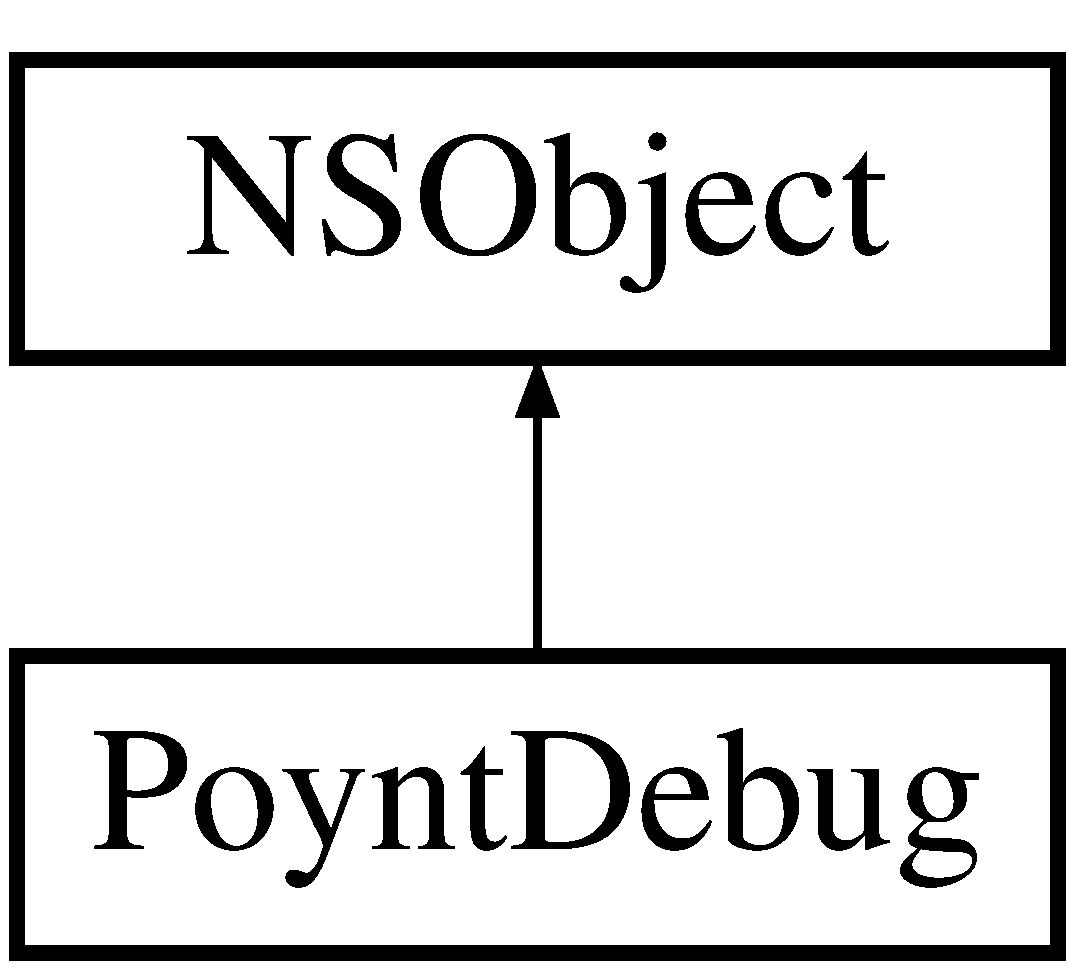
\includegraphics[height=2.000000cm]{interface_poynt_debug}
\end{center}
\end{figure}
\subsection*{Class Methods}
\begin{DoxyCompactItemize}
\item 
(\hyperlink{interface_poynt_debug}{Poynt\+Debug} $\ast$) + \hyperlink{interface_poynt_debug_a4dfaa75fbad98c4583833b43e18c0bbb}{shared\+Debugger}
\begin{DoxyCompactList}\small\item\em singleton property \end{DoxyCompactList}\item 
(void) + \hyperlink{interface_poynt_debug_a7a02ec4b1915a579185b23cc7d2e6b40}{log\+:}
\begin{DoxyCompactList}\small\item\em the log\+: method allows devlopers to take advantage of conditional verbose logging, sending your own message \end{DoxyCompactList}\end{DoxyCompactItemize}
\subsection*{Properties}
\begin{DoxyCompactItemize}
\item 
B\+O\+OL \hyperlink{interface_poynt_debug_ad023bbf13e60f8caee82c26f70e0f0a5}{verbose}
\begin{DoxyCompactList}\small\item\em set to true to see the magic, set to false to make your console look blank \end{DoxyCompactList}\end{DoxyCompactItemize}


\subsection{Detailed Description}
\hyperlink{interface_poynt_debug}{Poynt\+Debug}  Poynt\+Lib logs most requests , responses and errors. Use this class to see what your missing 

Definition at line 14 of file Poynt\+Debug.\+h.



\subsection{Method Documentation}
\hypertarget{interface_poynt_debug_a7a02ec4b1915a579185b23cc7d2e6b40}{}\label{interface_poynt_debug_a7a02ec4b1915a579185b23cc7d2e6b40} 
\index{Poynt\+Debug@{Poynt\+Debug}!log\+:@{log\+:}}
\index{log\+:@{log\+:}!Poynt\+Debug@{Poynt\+Debug}}
\subsubsection{\texorpdfstring{log\+:()}{log:()}}
{\footnotesize\ttfamily + (void) log\+: \begin{DoxyParamCaption}\item[{(N\+S\+String $\ast$)}]{message }\end{DoxyParamCaption}}



the log\+: method allows devlopers to take advantage of conditional verbose logging, sending your own message 

\hypertarget{interface_poynt_debug_a4dfaa75fbad98c4583833b43e18c0bbb}{}\label{interface_poynt_debug_a4dfaa75fbad98c4583833b43e18c0bbb} 
\index{Poynt\+Debug@{Poynt\+Debug}!shared\+Debugger@{shared\+Debugger}}
\index{shared\+Debugger@{shared\+Debugger}!Poynt\+Debug@{Poynt\+Debug}}
\subsubsection{\texorpdfstring{shared\+Debugger()}{sharedDebugger()}}
{\footnotesize\ttfamily + (\hyperlink{interface_poynt_debug}{Poynt\+Debug}$\ast$) shared\+Debugger \begin{DoxyParamCaption}{ }\end{DoxyParamCaption}}



singleton property 



\subsection{Property Documentation}
\hypertarget{interface_poynt_debug_ad023bbf13e60f8caee82c26f70e0f0a5}{}\label{interface_poynt_debug_ad023bbf13e60f8caee82c26f70e0f0a5} 
\index{Poynt\+Debug@{Poynt\+Debug}!verbose@{verbose}}
\index{verbose@{verbose}!Poynt\+Debug@{Poynt\+Debug}}
\subsubsection{\texorpdfstring{verbose}{verbose}}
{\footnotesize\ttfamily -\/ (B\+O\+OL) verbose\hspace{0.3cm}{\ttfamily [read]}, {\ttfamily [write]}, {\ttfamily [nonatomic]}, {\ttfamily [assign]}}



set to true to see the magic, set to false to make your console look blank 



Definition at line 22 of file Poynt\+Debug.\+h.



The documentation for this class was generated from the following file\+:\begin{DoxyCompactItemize}
\item 
Poynt\+Lib/\hyperlink{_poynt_debug_8h}{Poynt\+Debug.\+h}\end{DoxyCompactItemize}

\hypertarget{interface_poynt_discount_object}{}\section{Poynt\+Discount\+Object Class Reference}
\label{interface_poynt_discount_object}\index{Poynt\+Discount\+Object@{Poynt\+Discount\+Object}}


{\ttfamily \#import $<$Poynt\+Discount\+Object.\+h$>$}

Inheritance diagram for Poynt\+Discount\+Object\+:\begin{figure}[H]
\begin{center}
\leavevmode
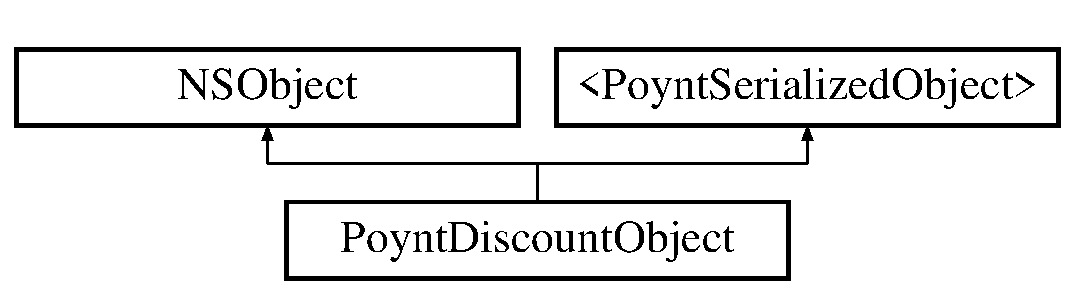
\includegraphics[height=2.000000cm]{interface_poynt_discount_object}
\end{center}
\end{figure}
\subsection*{Instance Methods}
\begin{DoxyCompactItemize}
\item 
(id) -\/ \hyperlink{interface_poynt_discount_object_aca2778db881b6bf8745ee57b1d4e7639}{init\+With\+Amount\+:custom\+Name\+:}
\begin{DoxyCompactList}\small\item\em initialize discount objects using the init\+With\+Amount or init. \end{DoxyCompactList}\end{DoxyCompactItemize}
\subsection*{Properties}
\begin{DoxyCompactItemize}
\item 
N\+S\+Integer \hyperlink{interface_poynt_discount_object_a6ff5079a7aa518c578773da69959732d}{amount}
\begin{DoxyCompactList}\small\item\em the amount in cents describing this discount \end{DoxyCompactList}\item 
N\+S\+String $\ast$ \hyperlink{interface_poynt_discount_object_ae38352d9ec7d2d1f03df4d4646c1a641}{custom\+Name}
\begin{DoxyCompactList}\small\item\em a human readable name for identifiying the meaning of this discount \end{DoxyCompactList}\end{DoxyCompactItemize}


\subsection{Detailed Description}
\hyperlink{interface_poynt_discount_object}{Poynt\+Discount\+Object}  discounts are encapsulated in an object to more easily identify their meaning.


\begin{DoxyCode}
\hyperlink{interface_poynt_discount_object}{PoyntDiscountObject} *discount  = [[\hyperlink{interface_poynt_discount_object}{PoyntDiscountObject} alloc] 
      initWithAmount:200 \hyperlink{interface_poynt_discount_object_ae38352d9ec7d2d1f03df4d4646c1a641}{customName}:\textcolor{stringliteral}{@"Customer Loyalty"}];
\end{DoxyCode}
 

Definition at line 19 of file Poynt\+Discount\+Object.\+h.



\subsection{Method Documentation}
\hypertarget{interface_poynt_discount_object_aca2778db881b6bf8745ee57b1d4e7639}{}\label{interface_poynt_discount_object_aca2778db881b6bf8745ee57b1d4e7639} 
\index{Poynt\+Discount\+Object@{Poynt\+Discount\+Object}!init\+With\+Amount\+:custom\+Name\+:@{init\+With\+Amount\+:custom\+Name\+:}}
\index{init\+With\+Amount\+:custom\+Name\+:@{init\+With\+Amount\+:custom\+Name\+:}!Poynt\+Discount\+Object@{Poynt\+Discount\+Object}}
\subsubsection{\texorpdfstring{init\+With\+Amount\+:custom\+Name\+:()}{initWithAmount:customName:()}}
{\footnotesize\ttfamily -\/ (id) init\+With\+Amount\+: \begin{DoxyParamCaption}\item[{(N\+S\+Integer)}]{amount }\item[{customName:(N\+S\+String $\ast$)}]{custom\+Name }\end{DoxyParamCaption}}



initialize discount objects using the init\+With\+Amount or init. 

\begin{DoxyNote}{Note}
Iniitializing with init will default amount to 0 and custom\+Name to an empty string 
\end{DoxyNote}


\subsection{Property Documentation}
\hypertarget{interface_poynt_discount_object_a6ff5079a7aa518c578773da69959732d}{}\label{interface_poynt_discount_object_a6ff5079a7aa518c578773da69959732d} 
\index{Poynt\+Discount\+Object@{Poynt\+Discount\+Object}!amount@{amount}}
\index{amount@{amount}!Poynt\+Discount\+Object@{Poynt\+Discount\+Object}}
\subsubsection{\texorpdfstring{amount}{amount}}
{\footnotesize\ttfamily -\/ (N\+S\+Integer) amount\hspace{0.3cm}{\ttfamily [read]}, {\ttfamily [write]}, {\ttfamily [nonatomic]}, {\ttfamily [assign]}}



the amount in cents describing this discount 



Definition at line 23 of file Poynt\+Discount\+Object.\+h.

\hypertarget{interface_poynt_discount_object_ae38352d9ec7d2d1f03df4d4646c1a641}{}\label{interface_poynt_discount_object_ae38352d9ec7d2d1f03df4d4646c1a641} 
\index{Poynt\+Discount\+Object@{Poynt\+Discount\+Object}!custom\+Name@{custom\+Name}}
\index{custom\+Name@{custom\+Name}!Poynt\+Discount\+Object@{Poynt\+Discount\+Object}}
\subsubsection{\texorpdfstring{custom\+Name}{customName}}
{\footnotesize\ttfamily -\/ (N\+S\+String$\ast$) custom\+Name\hspace{0.3cm}{\ttfamily [read]}, {\ttfamily [write]}, {\ttfamily [nonatomic]}, {\ttfamily [copy]}}



a human readable name for identifiying the meaning of this discount 



Definition at line 27 of file Poynt\+Discount\+Object.\+h.



The documentation for this class was generated from the following file\+:\begin{DoxyCompactItemize}
\item 
Poynt\+Lib/models/\hyperlink{_poynt_discount_object_8h}{Poynt\+Discount\+Object.\+h}\end{DoxyCompactItemize}

\hypertarget{interface_poynt_order_item_object}{}\section{Poynt\+Order\+Item\+Object Class Reference}
\label{interface_poynt_order_item_object}\index{Poynt\+Order\+Item\+Object@{Poynt\+Order\+Item\+Object}}


{\ttfamily \#import $<$Poynt\+Order\+Item\+Object.\+h$>$}

Inheritance diagram for Poynt\+Order\+Item\+Object\+:\begin{figure}[H]
\begin{center}
\leavevmode
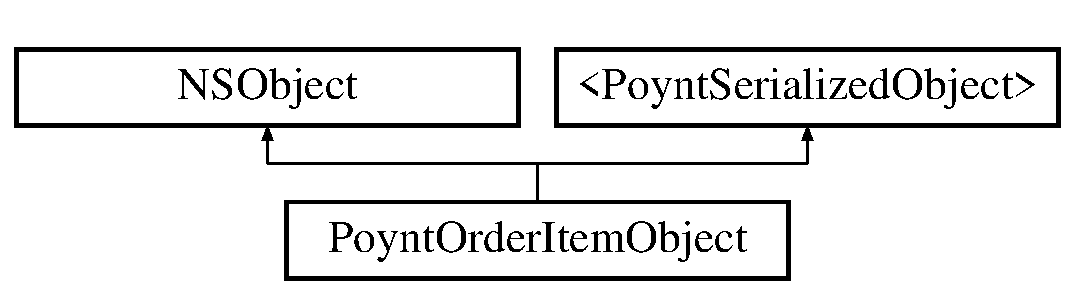
\includegraphics[height=2.000000cm]{interface_poynt_order_item_object}
\end{center}
\end{figure}
\subsection*{Instance Methods}
\begin{DoxyCompactItemize}
\item 
(id) -\/ \hyperlink{interface_poynt_order_item_object_a9af033018e30ae4ea14b2425c449e443}{init\+With\+Sku\+:unit\+Price\+:quantity\+:}
\begin{DoxyCompactList}\small\item\em initialization that will set the sku , unit\+Price and quantity \end{DoxyCompactList}\end{DoxyCompactItemize}
\subsection*{Properties}
\begin{DoxyCompactItemize}
\item 
N\+S\+String $\ast$ \hyperlink{interface_poynt_order_item_object_a1748706da6a2d9e7513e0075dadfc348}{client\+Notes}
\begin{DoxyCompactList}\small\item\em merchant notes for human readablity  the notes field can be used to document information that is not imperative, but useful to merchants \end{DoxyCompactList}\item 
N\+S\+Array $\ast$ \hyperlink{interface_poynt_order_item_object_a203259381417b0a34916ce3f864161c2}{discounts}
\begin{DoxyCompactList}\small\item\em array of \hyperlink{interface_poynt_discount_object}{Poynt\+Discount\+Object} objects  items can have multiple discounts for various reasons. Store them here \end{DoxyCompactList}\item 
N\+S\+String $\ast$ \hyperlink{interface_poynt_order_item_object_a4b93d352d2fca75b34e1b5a50e03f587}{name}
\begin{DoxyCompactList}\small\item\em human friendly name for this item.  The name can be any string and does not need to be unique \end{DoxyCompactList}\item 
N\+S\+String $\ast$ \hyperlink{interface_poynt_order_item_object_a40fae7616715aeb5f241af769a5f55b4}{sku}
\begin{DoxyCompactList}\small\item\em sku  Sku of the item. \end{DoxyCompactList}\item 
N\+S\+String $\ast$ \hyperlink{interface_poynt_order_item_object_ac2acf327011ce6ed9e26a41ceddaee31}{status}
\begin{DoxyCompactList}\small\item\em Status of the item  this is traditionaly set by the system and is likely \textquotesingle{}O\+R\+D\+E\+R\+ED\textquotesingle{}, \textquotesingle{}F\+U\+L\+F\+I\+L\+L\+ED\textquotesingle{}, \textquotesingle{}R\+E\+T\+U\+R\+N\+ED\textquotesingle{}. \end{DoxyCompactList}\item 
N\+S\+Array $\ast$ \hyperlink{interface_poynt_order_item_object_a24101b932074a386b535ab58e819bf71}{taxes}
\begin{DoxyCompactList}\small\item\em array of \hyperlink{interface_poynt_order_item_tax}{Poynt\+Order\+Item\+Tax} objects  like discounts, various taxes may be applied to an item \end{DoxyCompactList}\item 
\hyperlink{_poynt_order_item_object_8h_a7a5dd044bd57739d1d1b3e3565fbac25}{Unit\+Of\+Measure} \hyperlink{interface_poynt_order_item_object_a8381a2b60fb912bab67a5218ba3ad058}{unit\+Of\+Measure}
\begin{DoxyCompactList}\small\item\em Unit\+Of\+Measure  Unit of measure for the quantity. \end{DoxyCompactList}\item 
N\+S\+Integer \hyperlink{interface_poynt_order_item_object_a4655acbe158688f583828a9a3b61a6aa}{unit\+Price}
\begin{DoxyCompactList}\small\item\em price per item in cents \end{DoxyCompactList}\item 
float \hyperlink{interface_poynt_order_item_object_ab39715c10682638e342e25893caa7372}{quantity}
\begin{DoxyCompactList}\small\item\em Quantity purchased.  Note this could be in decimals, e.\+g. 2.\+3 Kgs. \end{DoxyCompactList}\item 
N\+S\+Integer \hyperlink{interface_poynt_order_item_object_a23a4b2c80d04d250fb56741b46a2cb0d}{tax}
\begin{DoxyCompactList}\small\item\em Total tax amount applied on this group of items (not just 1 unit).  If not specified, but the taxes array is present the server will automatically sum up the amounts in taxes array and populate this. If not specified and taxes array is empty, this will default to 0. \end{DoxyCompactList}\end{DoxyCompactItemize}


\subsection{Detailed Description}
\hyperlink{interface_poynt_order_item_object}{Poynt\+Order\+Item\+Object}  order items are essential for the makeup of a \hyperlink{interface_poynt_payment_object}{Poynt\+Payment\+Object}. All order items declare their amount (in cents) and other details attached to accurately describe payments


\begin{DoxyCode}
\hyperlink{interface_poynt_order_item_object}{PoyntOrderItemObject} *item  = [[\hyperlink{interface_poynt_order_item_object}{PoyntOrderItemObject} alloc] 
      initWithSku:\textcolor{stringliteral}{"unique.sku.name"} \hyperlink{interface_poynt_order_item_object_a4655acbe158688f583828a9a3b61a6aa}{unitPrice}:200 \hyperlink{interface_poynt_order_item_object_ab39715c10682638e342e25893caa7372}{quantity}:2.1];
\end{DoxyCode}
 

Definition at line 54 of file Poynt\+Order\+Item\+Object.\+h.



\subsection{Method Documentation}
\hypertarget{interface_poynt_order_item_object_a9af033018e30ae4ea14b2425c449e443}{}\label{interface_poynt_order_item_object_a9af033018e30ae4ea14b2425c449e443} 
\index{Poynt\+Order\+Item\+Object@{Poynt\+Order\+Item\+Object}!init\+With\+Sku\+:unit\+Price\+:quantity\+:@{init\+With\+Sku\+:unit\+Price\+:quantity\+:}}
\index{init\+With\+Sku\+:unit\+Price\+:quantity\+:@{init\+With\+Sku\+:unit\+Price\+:quantity\+:}!Poynt\+Order\+Item\+Object@{Poynt\+Order\+Item\+Object}}
\subsubsection{\texorpdfstring{init\+With\+Sku\+:unit\+Price\+:quantity\+:()}{initWithSku:unitPrice:quantity:()}}
{\footnotesize\ttfamily -\/ (id) init\+With\+Sku\+: \begin{DoxyParamCaption}\item[{(N\+S\+String $\ast$)}]{sku }\item[{unitPrice:(N\+S\+Integer)}]{unit\+Price }\item[{quantity:(float)}]{quantity }\end{DoxyParamCaption}}



initialization that will set the sku , unit\+Price and quantity 



\subsection{Property Documentation}
\hypertarget{interface_poynt_order_item_object_a1748706da6a2d9e7513e0075dadfc348}{}\label{interface_poynt_order_item_object_a1748706da6a2d9e7513e0075dadfc348} 
\index{Poynt\+Order\+Item\+Object@{Poynt\+Order\+Item\+Object}!client\+Notes@{client\+Notes}}
\index{client\+Notes@{client\+Notes}!Poynt\+Order\+Item\+Object@{Poynt\+Order\+Item\+Object}}
\subsubsection{\texorpdfstring{client\+Notes}{clientNotes}}
{\footnotesize\ttfamily -\/ (N\+S\+String$\ast$) client\+Notes\hspace{0.3cm}{\ttfamily [read]}, {\ttfamily [write]}, {\ttfamily [nonatomic]}, {\ttfamily [copy]}}



merchant notes for human readablity  the notes field can be used to document information that is not imperative, but useful to merchants 



Definition at line 59 of file Poynt\+Order\+Item\+Object.\+h.

\hypertarget{interface_poynt_order_item_object_a203259381417b0a34916ce3f864161c2}{}\label{interface_poynt_order_item_object_a203259381417b0a34916ce3f864161c2} 
\index{Poynt\+Order\+Item\+Object@{Poynt\+Order\+Item\+Object}!discounts@{discounts}}
\index{discounts@{discounts}!Poynt\+Order\+Item\+Object@{Poynt\+Order\+Item\+Object}}
\subsubsection{\texorpdfstring{discounts}{discounts}}
{\footnotesize\ttfamily -\/ (N\+S\+Array$\ast$) discounts\hspace{0.3cm}{\ttfamily [read]}, {\ttfamily [write]}, {\ttfamily [nonatomic]}, {\ttfamily [strong]}}



array of \hyperlink{interface_poynt_discount_object}{Poynt\+Discount\+Object} objects  items can have multiple discounts for various reasons. Store them here 



Definition at line 64 of file Poynt\+Order\+Item\+Object.\+h.

\hypertarget{interface_poynt_order_item_object_a4b93d352d2fca75b34e1b5a50e03f587}{}\label{interface_poynt_order_item_object_a4b93d352d2fca75b34e1b5a50e03f587} 
\index{Poynt\+Order\+Item\+Object@{Poynt\+Order\+Item\+Object}!name@{name}}
\index{name@{name}!Poynt\+Order\+Item\+Object@{Poynt\+Order\+Item\+Object}}
\subsubsection{\texorpdfstring{name}{name}}
{\footnotesize\ttfamily -\/ (N\+S\+String$\ast$) name\hspace{0.3cm}{\ttfamily [read]}, {\ttfamily [write]}, {\ttfamily [nonatomic]}, {\ttfamily [copy]}}



human friendly name for this item.  The name can be any string and does not need to be unique 



Definition at line 69 of file Poynt\+Order\+Item\+Object.\+h.

\hypertarget{interface_poynt_order_item_object_ab39715c10682638e342e25893caa7372}{}\label{interface_poynt_order_item_object_ab39715c10682638e342e25893caa7372} 
\index{Poynt\+Order\+Item\+Object@{Poynt\+Order\+Item\+Object}!quantity@{quantity}}
\index{quantity@{quantity}!Poynt\+Order\+Item\+Object@{Poynt\+Order\+Item\+Object}}
\subsubsection{\texorpdfstring{quantity}{quantity}}
{\footnotesize\ttfamily -\/ (float) quantity\hspace{0.3cm}{\ttfamily [read]}, {\ttfamily [write]}, {\ttfamily [nonatomic]}, {\ttfamily [assign]}}



Quantity purchased.  Note this could be in decimals, e.\+g. 2.\+3 Kgs. 



Definition at line 98 of file Poynt\+Order\+Item\+Object.\+h.

\hypertarget{interface_poynt_order_item_object_a40fae7616715aeb5f241af769a5f55b4}{}\label{interface_poynt_order_item_object_a40fae7616715aeb5f241af769a5f55b4} 
\index{Poynt\+Order\+Item\+Object@{Poynt\+Order\+Item\+Object}!sku@{sku}}
\index{sku@{sku}!Poynt\+Order\+Item\+Object@{Poynt\+Order\+Item\+Object}}
\subsubsection{\texorpdfstring{sku}{sku}}
{\footnotesize\ttfamily -\/ (N\+S\+String$\ast$) sku\hspace{0.3cm}{\ttfamily [read]}, {\ttfamily [write]}, {\ttfamily [nonatomic]}, {\ttfamily [copy]}}



sku  Sku of the item. 



Definition at line 74 of file Poynt\+Order\+Item\+Object.\+h.

\hypertarget{interface_poynt_order_item_object_ac2acf327011ce6ed9e26a41ceddaee31}{}\label{interface_poynt_order_item_object_ac2acf327011ce6ed9e26a41ceddaee31} 
\index{Poynt\+Order\+Item\+Object@{Poynt\+Order\+Item\+Object}!status@{status}}
\index{status@{status}!Poynt\+Order\+Item\+Object@{Poynt\+Order\+Item\+Object}}
\subsubsection{\texorpdfstring{status}{status}}
{\footnotesize\ttfamily -\/ (N\+S\+String$\ast$) status\hspace{0.3cm}{\ttfamily [read]}, {\ttfamily [write]}, {\ttfamily [nonatomic]}, {\ttfamily [copy]}}



Status of the item  this is traditionaly set by the system and is likely \textquotesingle{}O\+R\+D\+E\+R\+ED\textquotesingle{}, \textquotesingle{}F\+U\+L\+F\+I\+L\+L\+ED\textquotesingle{}, \textquotesingle{}R\+E\+T\+U\+R\+N\+ED\textquotesingle{}. 



Definition at line 79 of file Poynt\+Order\+Item\+Object.\+h.

\hypertarget{interface_poynt_order_item_object_a23a4b2c80d04d250fb56741b46a2cb0d}{}\label{interface_poynt_order_item_object_a23a4b2c80d04d250fb56741b46a2cb0d} 
\index{Poynt\+Order\+Item\+Object@{Poynt\+Order\+Item\+Object}!tax@{tax}}
\index{tax@{tax}!Poynt\+Order\+Item\+Object@{Poynt\+Order\+Item\+Object}}
\subsubsection{\texorpdfstring{tax}{tax}}
{\footnotesize\ttfamily -\/ (N\+S\+Integer) tax\hspace{0.3cm}{\ttfamily [read]}, {\ttfamily [nonatomic]}, {\ttfamily [assign]}}



Total tax amount applied on this group of items (not just 1 unit).  If not specified, but the taxes array is present the server will automatically sum up the amounts in taxes array and populate this. If not specified and taxes array is empty, this will default to 0. 



Definition at line 103 of file Poynt\+Order\+Item\+Object.\+h.

\hypertarget{interface_poynt_order_item_object_a24101b932074a386b535ab58e819bf71}{}\label{interface_poynt_order_item_object_a24101b932074a386b535ab58e819bf71} 
\index{Poynt\+Order\+Item\+Object@{Poynt\+Order\+Item\+Object}!taxes@{taxes}}
\index{taxes@{taxes}!Poynt\+Order\+Item\+Object@{Poynt\+Order\+Item\+Object}}
\subsubsection{\texorpdfstring{taxes}{taxes}}
{\footnotesize\ttfamily -\/ (N\+S\+Array$\ast$) taxes\hspace{0.3cm}{\ttfamily [read]}, {\ttfamily [write]}, {\ttfamily [nonatomic]}, {\ttfamily [strong]}}



array of \hyperlink{interface_poynt_order_item_tax}{Poynt\+Order\+Item\+Tax} objects  like discounts, various taxes may be applied to an item 



Definition at line 84 of file Poynt\+Order\+Item\+Object.\+h.

\hypertarget{interface_poynt_order_item_object_a8381a2b60fb912bab67a5218ba3ad058}{}\label{interface_poynt_order_item_object_a8381a2b60fb912bab67a5218ba3ad058} 
\index{Poynt\+Order\+Item\+Object@{Poynt\+Order\+Item\+Object}!unit\+Of\+Measure@{unit\+Of\+Measure}}
\index{unit\+Of\+Measure@{unit\+Of\+Measure}!Poynt\+Order\+Item\+Object@{Poynt\+Order\+Item\+Object}}
\subsubsection{\texorpdfstring{unit\+Of\+Measure}{unitOfMeasure}}
{\footnotesize\ttfamily -\/ (\hyperlink{_poynt_order_item_object_8h_a7a5dd044bd57739d1d1b3e3565fbac25}{Unit\+Of\+Measure}) unit\+Of\+Measure\hspace{0.3cm}{\ttfamily [read]}, {\ttfamily [write]}, {\ttfamily [nonatomic]}, {\ttfamily [assign]}}



Unit\+Of\+Measure  Unit of measure for the quantity. 



Definition at line 89 of file Poynt\+Order\+Item\+Object.\+h.

\hypertarget{interface_poynt_order_item_object_a4655acbe158688f583828a9a3b61a6aa}{}\label{interface_poynt_order_item_object_a4655acbe158688f583828a9a3b61a6aa} 
\index{Poynt\+Order\+Item\+Object@{Poynt\+Order\+Item\+Object}!unit\+Price@{unit\+Price}}
\index{unit\+Price@{unit\+Price}!Poynt\+Order\+Item\+Object@{Poynt\+Order\+Item\+Object}}
\subsubsection{\texorpdfstring{unit\+Price}{unitPrice}}
{\footnotesize\ttfamily -\/ (N\+S\+Integer) unit\+Price\hspace{0.3cm}{\ttfamily [read]}, {\ttfamily [write]}, {\ttfamily [nonatomic]}, {\ttfamily [assign]}}



price per item in cents 



Definition at line 93 of file Poynt\+Order\+Item\+Object.\+h.



The documentation for this class was generated from the following file\+:\begin{DoxyCompactItemize}
\item 
Poynt\+Lib/models/\hyperlink{_poynt_order_item_object_8h}{Poynt\+Order\+Item\+Object.\+h}\end{DoxyCompactItemize}

\hypertarget{interface_poynt_order_item_tax}{}\section{Poynt\+Order\+Item\+Tax Class Reference}
\label{interface_poynt_order_item_tax}\index{Poynt\+Order\+Item\+Tax@{Poynt\+Order\+Item\+Tax}}


{\ttfamily \#import $<$Poynt\+Order\+Item\+Tax.\+h$>$}

Inheritance diagram for Poynt\+Order\+Item\+Tax\+:\begin{figure}[H]
\begin{center}
\leavevmode
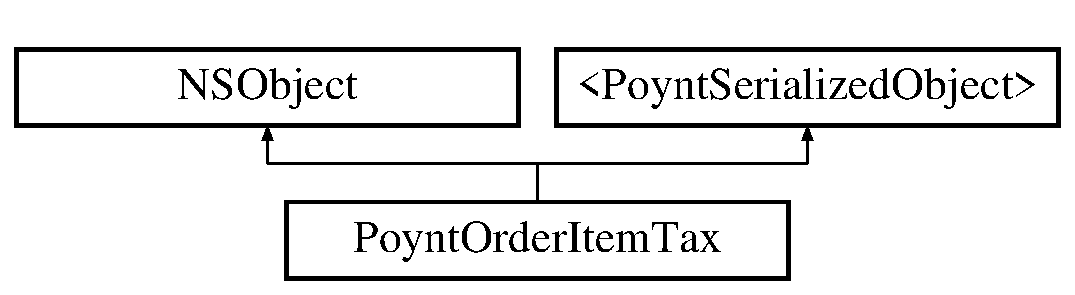
\includegraphics[height=2.000000cm]{interface_poynt_order_item_tax}
\end{center}
\end{figure}
\subsection*{Instance Methods}
\begin{DoxyCompactItemize}
\item 
(id) -\/ \hyperlink{interface_poynt_order_item_tax_a64b4adba02da4a202dd84d072ce7f644}{init\+With\+Amount\+:type\+:}
\begin{DoxyCompactList}\small\item\em only use init\+With\+Amount\+:type to create these objects to ensure the obligatory fields are populated \end{DoxyCompactList}\end{DoxyCompactItemize}
\subsection*{Properties}
\begin{DoxyCompactItemize}
\item 
N\+S\+String $\ast$ \hyperlink{interface_poynt_order_item_tax_a342356fc9b7bcfd0250df7e71bc2360e}{order\+Item\+Tax\+Id}
\begin{DoxyCompactList}\small\item\em string representing this id \end{DoxyCompactList}\item 
N\+S\+String $\ast$ \hyperlink{interface_poynt_order_item_tax_abff6a04d71c2bba87e646615388a1f5c}{type}
\begin{DoxyCompactList}\small\item\em string value representing the type of tax \end{DoxyCompactList}\item 
N\+S\+Integer \hyperlink{interface_poynt_order_item_tax_a6ff5079a7aa518c578773da69959732d}{amount}
\begin{DoxyCompactList}\small\item\em the amount of tax in cents \end{DoxyCompactList}\end{DoxyCompactItemize}


\subsection{Detailed Description}
\hyperlink{interface_poynt_order_item_tax}{Poynt\+Order\+Item\+Tax}  tax object associated to an item 

Definition at line 15 of file Poynt\+Order\+Item\+Tax.\+h.



\subsection{Method Documentation}
\hypertarget{interface_poynt_order_item_tax_a64b4adba02da4a202dd84d072ce7f644}{}\label{interface_poynt_order_item_tax_a64b4adba02da4a202dd84d072ce7f644} 
\index{Poynt\+Order\+Item\+Tax@{Poynt\+Order\+Item\+Tax}!init\+With\+Amount\+:type\+:@{init\+With\+Amount\+:type\+:}}
\index{init\+With\+Amount\+:type\+:@{init\+With\+Amount\+:type\+:}!Poynt\+Order\+Item\+Tax@{Poynt\+Order\+Item\+Tax}}
\subsubsection{\texorpdfstring{init\+With\+Amount\+:type\+:()}{initWithAmount:type:()}}
{\footnotesize\ttfamily -\/ (id) init\+With\+Amount\+: \begin{DoxyParamCaption}\item[{(N\+S\+Integer)}]{amount }\item[{type:(N\+S\+String $\ast$)}]{type }\end{DoxyParamCaption}}



only use init\+With\+Amount\+:type to create these objects to ensure the obligatory fields are populated 



\subsection{Property Documentation}
\hypertarget{interface_poynt_order_item_tax_a6ff5079a7aa518c578773da69959732d}{}\label{interface_poynt_order_item_tax_a6ff5079a7aa518c578773da69959732d} 
\index{Poynt\+Order\+Item\+Tax@{Poynt\+Order\+Item\+Tax}!amount@{amount}}
\index{amount@{amount}!Poynt\+Order\+Item\+Tax@{Poynt\+Order\+Item\+Tax}}
\subsubsection{\texorpdfstring{amount}{amount}}
{\footnotesize\ttfamily -\/ (N\+S\+Integer) amount\hspace{0.3cm}{\ttfamily [read]}, {\ttfamily [write]}, {\ttfamily [nonatomic]}, {\ttfamily [assign]}}



the amount of tax in cents 



Definition at line 27 of file Poynt\+Order\+Item\+Tax.\+h.

\hypertarget{interface_poynt_order_item_tax_a342356fc9b7bcfd0250df7e71bc2360e}{}\label{interface_poynt_order_item_tax_a342356fc9b7bcfd0250df7e71bc2360e} 
\index{Poynt\+Order\+Item\+Tax@{Poynt\+Order\+Item\+Tax}!order\+Item\+Tax\+Id@{order\+Item\+Tax\+Id}}
\index{order\+Item\+Tax\+Id@{order\+Item\+Tax\+Id}!Poynt\+Order\+Item\+Tax@{Poynt\+Order\+Item\+Tax}}
\subsubsection{\texorpdfstring{order\+Item\+Tax\+Id}{orderItemTaxId}}
{\footnotesize\ttfamily -\/ (N\+S\+String$\ast$) order\+Item\+Tax\+Id\hspace{0.3cm}{\ttfamily [read]}, {\ttfamily [write]}, {\ttfamily [nonatomic]}, {\ttfamily [copy]}}



string representing this id 



Definition at line 19 of file Poynt\+Order\+Item\+Tax.\+h.

\hypertarget{interface_poynt_order_item_tax_abff6a04d71c2bba87e646615388a1f5c}{}\label{interface_poynt_order_item_tax_abff6a04d71c2bba87e646615388a1f5c} 
\index{Poynt\+Order\+Item\+Tax@{Poynt\+Order\+Item\+Tax}!type@{type}}
\index{type@{type}!Poynt\+Order\+Item\+Tax@{Poynt\+Order\+Item\+Tax}}
\subsubsection{\texorpdfstring{type}{type}}
{\footnotesize\ttfamily -\/ (N\+S\+String$\ast$) type\hspace{0.3cm}{\ttfamily [read]}, {\ttfamily [write]}, {\ttfamily [nonatomic]}, {\ttfamily [copy]}}



string value representing the type of tax 



Definition at line 23 of file Poynt\+Order\+Item\+Tax.\+h.



The documentation for this class was generated from the following file\+:\begin{DoxyCompactItemize}
\item 
Poynt\+Lib/models/\hyperlink{_poynt_order_item_tax_8h}{Poynt\+Order\+Item\+Tax.\+h}\end{DoxyCompactItemize}

\hypertarget{interface_poynt_order_object}{}\section{Poynt\+Order\+Object Class Reference}
\label{interface_poynt_order_object}\index{Poynt\+Order\+Object@{Poynt\+Order\+Object}}


{\ttfamily \#import $<$Poynt\+Order\+Object.\+h$>$}

Inheritance diagram for Poynt\+Order\+Object\+:\begin{figure}[H]
\begin{center}
\leavevmode
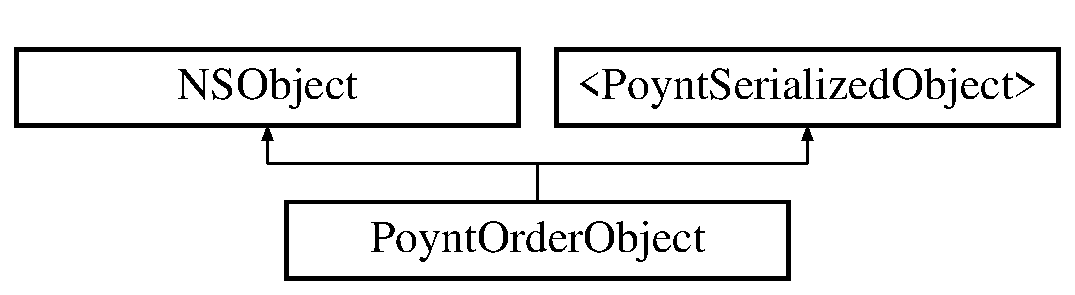
\includegraphics[height=2.000000cm]{interface_poynt_order_object}
\end{center}
\end{figure}
\subsection*{Properties}
\begin{DoxyCompactItemize}
\item 
N\+S\+String $\ast$ \hyperlink{interface_poynt_order_object_a940861134b75ee3d5167d791e5422afe}{notes}
\begin{DoxyCompactList}\small\item\em merchant notes for human readablity  the notes field can be used to document information that is not imperative, but useful to merchants \end{DoxyCompactList}\item 
N\+S\+String $\ast$ \hyperlink{interface_poynt_order_object_add3af147d846009706270bf6315b1229}{order\+Number}
\begin{DoxyCompactList}\small\item\em merchant friendly number identifier  Stores often use a human readable order number to hand out to customers. Such numbers could be passed here. \end{DoxyCompactList}\item 
\hyperlink{interface_poynt_payment_amount_object}{Poynt\+Payment\+Amount\+Object} $\ast$ \hyperlink{interface_poynt_order_object_a24782f14a239c62d29bf0389fb7fdf8d}{amounts}
\begin{DoxyCompactList}\small\item\em object store for tracking specifics about the amounts in payment  This object stores and calculates the pertant data that comprises the total, discount and tax of the order \end{DoxyCompactList}\item 
N\+S\+Array $\ast$ \hyperlink{interface_poynt_order_object_a203259381417b0a34916ce3f864161c2}{discounts}
\begin{DoxyCompactList}\small\item\em array of Poynt\+Discount\+Objects  The amounts object will use this collection in its calculations for describing totals associated to this order object \end{DoxyCompactList}\item 
N\+S\+Array $\ast$ \hyperlink{interface_poynt_order_object_a79b667618eb44106221f198156b54dd2}{items}
\begin{DoxyCompactList}\small\item\em array of \hyperlink{interface_poynt_order_item_object}{Poynt\+Order\+Item\+Object}  Orders contain at least one (or more) items. The amounts object will use this collection in its calculations for describing totals associated to this order object \end{DoxyCompactList}\item 
N\+S\+String $\ast$ \hyperlink{interface_poynt_order_object_aac2b120e80b4b9e69c3a577c4f31ed31}{order\+Id}
\begin{DoxyCompactList}\small\item\em system identifier for this object  The id of the order created. If provided in the request, it will be used as the order ID. If not provided, id will be generated internally. \end{DoxyCompactList}\end{DoxyCompactItemize}


\subsection{Detailed Description}
\hyperlink{interface_poynt_order_object}{Poynt\+Order\+Object}  Order objects are most commonly found attached to a \hyperlink{interface_poynt_payment_object}{Poynt\+Payment\+Object}. The order contains important information identifying itself in the system as well as items attached, discounts, and amounts 

Definition at line 18 of file Poynt\+Order\+Object.\+h.



\subsection{Property Documentation}
\hypertarget{interface_poynt_order_object_a24782f14a239c62d29bf0389fb7fdf8d}{}\label{interface_poynt_order_object_a24782f14a239c62d29bf0389fb7fdf8d} 
\index{Poynt\+Order\+Object@{Poynt\+Order\+Object}!amounts@{amounts}}
\index{amounts@{amounts}!Poynt\+Order\+Object@{Poynt\+Order\+Object}}
\subsubsection{\texorpdfstring{amounts}{amounts}}
{\footnotesize\ttfamily -\/ (\hyperlink{interface_poynt_payment_amount_object}{Poynt\+Payment\+Amount\+Object}$\ast$) amounts\hspace{0.3cm}{\ttfamily [read]}, {\ttfamily [write]}, {\ttfamily [nonatomic]}, {\ttfamily [strong]}}



object store for tracking specifics about the amounts in payment  This object stores and calculates the pertant data that comprises the total, discount and tax of the order 



Definition at line 33 of file Poynt\+Order\+Object.\+h.

\hypertarget{interface_poynt_order_object_a203259381417b0a34916ce3f864161c2}{}\label{interface_poynt_order_object_a203259381417b0a34916ce3f864161c2} 
\index{Poynt\+Order\+Object@{Poynt\+Order\+Object}!discounts@{discounts}}
\index{discounts@{discounts}!Poynt\+Order\+Object@{Poynt\+Order\+Object}}
\subsubsection{\texorpdfstring{discounts}{discounts}}
{\footnotesize\ttfamily -\/ (N\+S\+Array$\ast$) discounts\hspace{0.3cm}{\ttfamily [read]}, {\ttfamily [write]}, {\ttfamily [nonatomic]}, {\ttfamily [strong]}}



array of Poynt\+Discount\+Objects  The amounts object will use this collection in its calculations for describing totals associated to this order object 



Definition at line 38 of file Poynt\+Order\+Object.\+h.

\hypertarget{interface_poynt_order_object_a79b667618eb44106221f198156b54dd2}{}\label{interface_poynt_order_object_a79b667618eb44106221f198156b54dd2} 
\index{Poynt\+Order\+Object@{Poynt\+Order\+Object}!items@{items}}
\index{items@{items}!Poynt\+Order\+Object@{Poynt\+Order\+Object}}
\subsubsection{\texorpdfstring{items}{items}}
{\footnotesize\ttfamily -\/ (N\+S\+Array$\ast$) items\hspace{0.3cm}{\ttfamily [read]}, {\ttfamily [write]}, {\ttfamily [nonatomic]}, {\ttfamily [strong]}}



array of \hyperlink{interface_poynt_order_item_object}{Poynt\+Order\+Item\+Object}  Orders contain at least one (or more) items. The amounts object will use this collection in its calculations for describing totals associated to this order object 



Definition at line 43 of file Poynt\+Order\+Object.\+h.

\hypertarget{interface_poynt_order_object_a940861134b75ee3d5167d791e5422afe}{}\label{interface_poynt_order_object_a940861134b75ee3d5167d791e5422afe} 
\index{Poynt\+Order\+Object@{Poynt\+Order\+Object}!notes@{notes}}
\index{notes@{notes}!Poynt\+Order\+Object@{Poynt\+Order\+Object}}
\subsubsection{\texorpdfstring{notes}{notes}}
{\footnotesize\ttfamily -\/ (N\+S\+String$\ast$) notes\hspace{0.3cm}{\ttfamily [read]}, {\ttfamily [write]}, {\ttfamily [nonatomic]}, {\ttfamily [copy]}}



merchant notes for human readablity  the notes field can be used to document information that is not imperative, but useful to merchants 



Definition at line 23 of file Poynt\+Order\+Object.\+h.

\hypertarget{interface_poynt_order_object_aac2b120e80b4b9e69c3a577c4f31ed31}{}\label{interface_poynt_order_object_aac2b120e80b4b9e69c3a577c4f31ed31} 
\index{Poynt\+Order\+Object@{Poynt\+Order\+Object}!order\+Id@{order\+Id}}
\index{order\+Id@{order\+Id}!Poynt\+Order\+Object@{Poynt\+Order\+Object}}
\subsubsection{\texorpdfstring{order\+Id}{orderId}}
{\footnotesize\ttfamily -\/ (N\+S\+String$\ast$) order\+Id\hspace{0.3cm}{\ttfamily [read]}, {\ttfamily [write]}, {\ttfamily [nonatomic]}, {\ttfamily [copy]}}



system identifier for this object  The id of the order created. If provided in the request, it will be used as the order ID. If not provided, id will be generated internally. 



Definition at line 48 of file Poynt\+Order\+Object.\+h.

\hypertarget{interface_poynt_order_object_add3af147d846009706270bf6315b1229}{}\label{interface_poynt_order_object_add3af147d846009706270bf6315b1229} 
\index{Poynt\+Order\+Object@{Poynt\+Order\+Object}!order\+Number@{order\+Number}}
\index{order\+Number@{order\+Number}!Poynt\+Order\+Object@{Poynt\+Order\+Object}}
\subsubsection{\texorpdfstring{order\+Number}{orderNumber}}
{\footnotesize\ttfamily -\/ (N\+S\+String$\ast$) order\+Number\hspace{0.3cm}{\ttfamily [read]}, {\ttfamily [write]}, {\ttfamily [nonatomic]}, {\ttfamily [copy]}}



merchant friendly number identifier  Stores often use a human readable order number to hand out to customers. Such numbers could be passed here. 



Definition at line 28 of file Poynt\+Order\+Object.\+h.



The documentation for this class was generated from the following file\+:\begin{DoxyCompactItemize}
\item 
Poynt\+Lib/models/\hyperlink{_poynt_order_object_8h}{Poynt\+Order\+Object.\+h}\end{DoxyCompactItemize}

\hypertarget{interface_poynt_payment_amount_object}{}\section{Poynt\+Payment\+Amount\+Object Class Reference}
\label{interface_poynt_payment_amount_object}\index{Poynt\+Payment\+Amount\+Object@{Poynt\+Payment\+Amount\+Object}}


{\ttfamily \#import $<$Poynt\+Payment\+Amount\+Object.\+h$>$}

Inheritance diagram for Poynt\+Payment\+Amount\+Object\+:\begin{figure}[H]
\begin{center}
\leavevmode
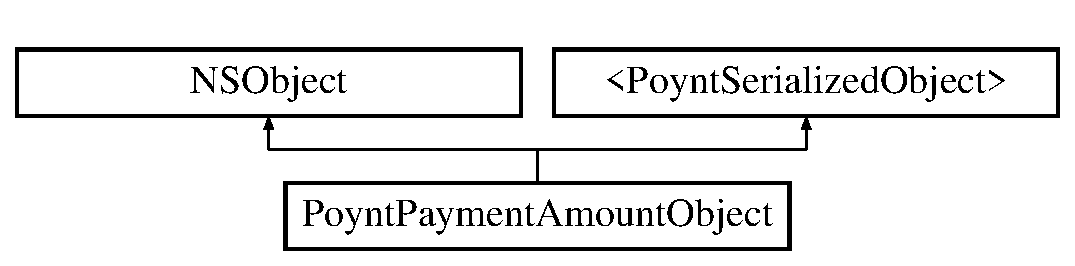
\includegraphics[height=2.000000cm]{interface_poynt_payment_amount_object}
\end{center}
\end{figure}
\subsection*{Instance Methods}
\begin{DoxyCompactItemize}
\item 
(void) -\/ \hyperlink{interface_poynt_payment_amount_object_a1c43473c035627846e64fddfb2bbe57d}{calculate\+:}
\begin{DoxyCompactList}\small\item\em call the calculate method to refresh the properites of this object. The S\+DK occasionly calls calculate on this object, and will always call for a fresh calculation immediately before sending a request to the terminal. \end{DoxyCompactList}\end{DoxyCompactItemize}
\subsection*{Properties}
\begin{DoxyCompactItemize}
\item 
N\+S\+Integer \hyperlink{interface_poynt_payment_amount_object_a6d7b64fe4a742c91067809f34bb7d2a2}{sub\+Total}
\begin{DoxyCompactList}\small\item\em total sum of unit\+Price $\ast$ quantity for each item in and order \end{DoxyCompactList}\item 
N\+S\+Integer \hyperlink{interface_poynt_payment_amount_object_a8a8c1f8f98bf7dc619baeb011a92aa93}{discount\+Total}
\begin{DoxyCompactList}\small\item\em total sum of discounts for each item in and order plus sum of discounts applied to the order itself \end{DoxyCompactList}\item 
N\+S\+Integer \hyperlink{interface_poynt_payment_amount_object_a86fed8c7d04bd309d6af2d0e75942163}{tax\+Total}
\begin{DoxyCompactList}\small\item\em total sum of tax for each item in and order \end{DoxyCompactList}\item 
N\+S\+String $\ast$ \hyperlink{interface_poynt_payment_amount_object_a71a9104f71558df8791cedc5e81941a3}{currency}
\begin{DoxyCompactList}\small\item\em currency of this payment amount  this field defaults to U\+SD. When attached to an order descended from a payment, it will inherit currency from the order\textquotesingle{}s payment object \end{DoxyCompactList}\end{DoxyCompactItemize}


\subsection{Detailed Description}
\hyperlink{interface_poynt_payment_amount_object}{Poynt\+Payment\+Amount\+Object}  the payment amount storage object responsible for calculating totals , taxes and discounts for a \hyperlink{interface_poynt_order_object}{Poynt\+Order\+Object} 

Definition at line 16 of file Poynt\+Payment\+Amount\+Object.\+h.



\subsection{Method Documentation}
\hypertarget{interface_poynt_payment_amount_object_a1c43473c035627846e64fddfb2bbe57d}{}\label{interface_poynt_payment_amount_object_a1c43473c035627846e64fddfb2bbe57d} 
\index{Poynt\+Payment\+Amount\+Object@{Poynt\+Payment\+Amount\+Object}!calculate\+:@{calculate\+:}}
\index{calculate\+:@{calculate\+:}!Poynt\+Payment\+Amount\+Object@{Poynt\+Payment\+Amount\+Object}}
\subsubsection{\texorpdfstring{calculate\+:()}{calculate:()}}
{\footnotesize\ttfamily -\/ (void) calculate\+: \begin{DoxyParamCaption}\item[{(\hyperlink{interface_poynt_order_object}{Poynt\+Order\+Object} $\ast$)}]{order }\end{DoxyParamCaption}}



call the calculate method to refresh the properites of this object. The S\+DK occasionly calls calculate on this object, and will always call for a fresh calculation immediately before sending a request to the terminal. 



\subsection{Property Documentation}
\hypertarget{interface_poynt_payment_amount_object_a71a9104f71558df8791cedc5e81941a3}{}\label{interface_poynt_payment_amount_object_a71a9104f71558df8791cedc5e81941a3} 
\index{Poynt\+Payment\+Amount\+Object@{Poynt\+Payment\+Amount\+Object}!currency@{currency}}
\index{currency@{currency}!Poynt\+Payment\+Amount\+Object@{Poynt\+Payment\+Amount\+Object}}
\subsubsection{\texorpdfstring{currency}{currency}}
{\footnotesize\ttfamily -\/ (N\+S\+String$\ast$) currency\hspace{0.3cm}{\ttfamily [read]}, {\ttfamily [write]}, {\ttfamily [nonatomic]}, {\ttfamily [strong]}}



currency of this payment amount  this field defaults to U\+SD. When attached to an order descended from a payment, it will inherit currency from the order\textquotesingle{}s payment object 



Definition at line 33 of file Poynt\+Payment\+Amount\+Object.\+h.

\hypertarget{interface_poynt_payment_amount_object_a8a8c1f8f98bf7dc619baeb011a92aa93}{}\label{interface_poynt_payment_amount_object_a8a8c1f8f98bf7dc619baeb011a92aa93} 
\index{Poynt\+Payment\+Amount\+Object@{Poynt\+Payment\+Amount\+Object}!discount\+Total@{discount\+Total}}
\index{discount\+Total@{discount\+Total}!Poynt\+Payment\+Amount\+Object@{Poynt\+Payment\+Amount\+Object}}
\subsubsection{\texorpdfstring{discount\+Total}{discountTotal}}
{\footnotesize\ttfamily -\/ (N\+S\+Integer) discount\+Total\hspace{0.3cm}{\ttfamily [read]}, {\ttfamily [write]}, {\ttfamily [nonatomic]}, {\ttfamily [assign]}}



total sum of discounts for each item in and order plus sum of discounts applied to the order itself 



Definition at line 24 of file Poynt\+Payment\+Amount\+Object.\+h.

\hypertarget{interface_poynt_payment_amount_object_a6d7b64fe4a742c91067809f34bb7d2a2}{}\label{interface_poynt_payment_amount_object_a6d7b64fe4a742c91067809f34bb7d2a2} 
\index{Poynt\+Payment\+Amount\+Object@{Poynt\+Payment\+Amount\+Object}!sub\+Total@{sub\+Total}}
\index{sub\+Total@{sub\+Total}!Poynt\+Payment\+Amount\+Object@{Poynt\+Payment\+Amount\+Object}}
\subsubsection{\texorpdfstring{sub\+Total}{subTotal}}
{\footnotesize\ttfamily -\/ (N\+S\+Integer) sub\+Total\hspace{0.3cm}{\ttfamily [read]}, {\ttfamily [write]}, {\ttfamily [nonatomic]}, {\ttfamily [assign]}}



total sum of unit\+Price $\ast$ quantity for each item in and order 



Definition at line 20 of file Poynt\+Payment\+Amount\+Object.\+h.

\hypertarget{interface_poynt_payment_amount_object_a86fed8c7d04bd309d6af2d0e75942163}{}\label{interface_poynt_payment_amount_object_a86fed8c7d04bd309d6af2d0e75942163} 
\index{Poynt\+Payment\+Amount\+Object@{Poynt\+Payment\+Amount\+Object}!tax\+Total@{tax\+Total}}
\index{tax\+Total@{tax\+Total}!Poynt\+Payment\+Amount\+Object@{Poynt\+Payment\+Amount\+Object}}
\subsubsection{\texorpdfstring{tax\+Total}{taxTotal}}
{\footnotesize\ttfamily -\/ (N\+S\+Integer) tax\+Total\hspace{0.3cm}{\ttfamily [read]}, {\ttfamily [write]}, {\ttfamily [nonatomic]}, {\ttfamily [assign]}}



total sum of tax for each item in and order 



Definition at line 28 of file Poynt\+Payment\+Amount\+Object.\+h.



The documentation for this class was generated from the following file\+:\begin{DoxyCompactItemize}
\item 
Poynt\+Lib/models/\hyperlink{_poynt_payment_amount_object_8h}{Poynt\+Payment\+Amount\+Object.\+h}\end{DoxyCompactItemize}

\hypertarget{interface_poynt_payment_object}{}\section{Poynt\+Payment\+Object Class Reference}
\label{interface_poynt_payment_object}\index{Poynt\+Payment\+Object@{Poynt\+Payment\+Object}}


The \hyperlink{interface_poynt_payment_object}{Poynt\+Payment\+Object} is the required parameter for many sale and presales requests. The object can be built before making requests to the terminal.  




{\ttfamily \#import $<$Poynt\+Payment\+Object.\+h$>$}

Inheritance diagram for Poynt\+Payment\+Object\+:\begin{figure}[H]
\begin{center}
\leavevmode
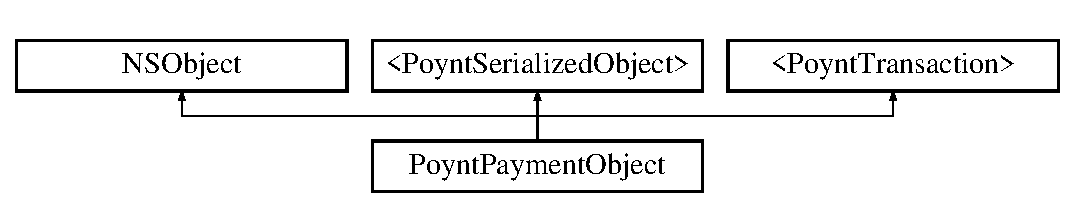
\includegraphics[height=2.000000cm]{interface_poynt_payment_object}
\end{center}
\end{figure}
\subsection*{Instance Methods}
\begin{DoxyCompactItemize}
\item 
(void) -\/ \hyperlink{interface_poynt_payment_object_ac5c54df7ed3b930268c8d7752c101725}{update}
\begin{DoxyCompactList}\small\item\em a method used to refresh the payment object  This method is most commonly run when the objec it about to send to terminal. It can be manually updated at anytime to refresh the absolute calculations \end{DoxyCompactList}\end{DoxyCompactItemize}
\subsection*{Properties}
\begin{DoxyCompactItemize}
\item 
N\+S\+Integer \hyperlink{interface_poynt_payment_object_a6ff5079a7aa518c578773da69959732d}{amount}
\begin{DoxyCompactList}\small\item\em the total amount of this object  The amount field should only be explicitly set when requesting a partial refund or partial completion. Otherwise this field is calculated from an attached \hyperlink{interface_poynt_order_object}{Poynt\+Order\+Object} \end{DoxyCompactList}\item 
\hyperlink{interface_poynt_payment_amount_object}{Poynt\+Payment\+Amount\+Object} $\ast$ \hyperlink{interface_poynt_payment_object_a24782f14a239c62d29bf0389fb7fdf8d}{amounts}
\begin{DoxyCompactList}\small\item\em a summary object for understanding details of an amount  The object is most closely related to orders, but can also be found in the \hyperlink{interface_poynt_payment_object}{Poynt\+Payment\+Object} \end{DoxyCompactList}\item 
N\+S\+Integer \hyperlink{interface_poynt_payment_object_a84de6fd790c3129d6d0a271d915d442a}{cashback}
\begin{DoxyCompactList}\small\item\em representation of amount cashback in payment  The value that is returned (in cents) for a payment transaction. \end{DoxyCompactList}\item 
B\+O\+OL \hyperlink{interface_poynt_payment_object_a7b74d30854a9218712b55c79cd7786f0}{cash\+Only}
\begin{DoxyCompactList}\small\item\em if the payment was cash only \end{DoxyCompactList}\item 
N\+S\+String $\ast$ \hyperlink{interface_poynt_payment_object_a71a9104f71558df8791cedc5e81941a3}{currency}
\begin{DoxyCompactList}\small\item\em representation for the currency of this payment \end{DoxyCompactList}\item 
B\+O\+OL \hyperlink{interface_poynt_payment_object_a76dfb16e254da2dd51a3269700a40581}{debit}
\begin{DoxyCompactList}\small\item\em if the payment uses debit \end{DoxyCompactList}\item 
B\+O\+OL \hyperlink{interface_poynt_payment_object_af4d70322e9072299e80fa78a54e7094e}{disable\+Cash}
\begin{DoxyCompactList}\small\item\em if the payment will allow cash \end{DoxyCompactList}\item 
B\+O\+OL \hyperlink{interface_poynt_payment_object_a3f9d08fa34a1f60c5818a7b570d8b41f}{disable\+Debit\+Cards}
\begin{DoxyCompactList}\small\item\em if the payment will disable debit cards \end{DoxyCompactList}\item 
B\+O\+OL \hyperlink{interface_poynt_payment_object_a7b291056797beff707e48865aefe7c5a}{disable\+Tip}
\begin{DoxyCompactList}\small\item\em if the payment will allow a tip \end{DoxyCompactList}\item 
B\+O\+OL \hyperlink{interface_poynt_payment_object_a42f2647ecd1d090fad6a7b77e28ee013}{multi\+Tender}
\begin{DoxyCompactList}\small\item\em if the payment uses multiple tenders to complete the transaction \end{DoxyCompactList}\item 
B\+O\+OL \hyperlink{interface_poynt_payment_object_a84b5ff3701d66e70a3bb2485d4e99a3b}{non\+Referenced\+Credit}
\begin{DoxyCompactList}\small\item\em if the payment of no referenced credit \end{DoxyCompactList}\item 
\hyperlink{interface_poynt_order_object}{Poynt\+Order\+Object} $\ast$ \hyperlink{interface_poynt_payment_object_a570f3f5a3eb312987a97d46c0ba10a9d}{order}
\begin{DoxyCompactList}\small\item\em the attached order object  The \hyperlink{interface_poynt_order_object}{Poynt\+Order\+Object} is an essential piece of a payment object as it contains the items and calculation components for understanding a payments values \end{DoxyCompactList}\item 
N\+S\+String $\ast$ \hyperlink{interface_poynt_payment_object_aac2b120e80b4b9e69c3a577c4f31ed31}{order\+Id}
\begin{DoxyCompactList}\small\item\em the order id  The payment object will auto generate an order id at init. The value of this can be kept of explicitly declared \end{DoxyCompactList}\item 
N\+S\+String $\ast$ \hyperlink{interface_poynt_payment_object_ab9a55f2b8aef17222c41f356957e2513}{reference\+Id}
\begin{DoxyCompactList}\small\item\em the reference id  The payment object will auto generate a reference id at init. The value of this can be kept of explicitly declared \end{DoxyCompactList}\item 
N\+S\+String $\ast$ \hyperlink{interface_poynt_payment_object_aacd11580c330a78310c344d78baecf8c}{transaction\+Id}
\begin{DoxyCompactList}\small\item\em the transaction id  The payment object will auto generate a transaction id at init. The value of this can be kept of explicitly declared. It is most common to explictly set this for partial actions (ie\+: Authorize\+Partial\+Refund or Authorize\+Partial\+Capture) \end{DoxyCompactList}\item 
B\+O\+OL \hyperlink{interface_poynt_payment_object_a065f8677ebd1da13c2f57bd6cbbf3d7c}{skip\+Receipt\+Screen}
\begin{DoxyCompactList}\small\item\em should the payment skip the receipt screen on the terminal after processing. \end{DoxyCompactList}\item 
N\+S\+Integer \hyperlink{interface_poynt_payment_object_ae4a2e64d79032bc8bb25305486b23859}{tip\+Amount}
\begin{DoxyCompactList}\small\item\em the amount being tipped (if any)  If there is a tip, it should be set here (in cents) \end{DoxyCompactList}\item 
N\+S\+Array $\ast$ \hyperlink{interface_poynt_payment_object_a12474d50a1838843bcc1cacbbc30c4d2}{transactions}
\begin{DoxyCompactList}\small\item\em collection of \hyperlink{interface_poynt_transaction_object}{Poynt\+Transaction\+Object}  A payment can consist of many transactions. \end{DoxyCompactList}\item 
N\+S\+Integer \hyperlink{interface_poynt_payment_object_aa5f2d0bac6ddbb63f1ada849fd4609d2}{absolute\+Discount\+Total}
\begin{DoxyCompactList}\small\item\em readonly property of calculated discount totals. \end{DoxyCompactList}\item 
N\+S\+Integer \hyperlink{interface_poynt_payment_object_a94b92d7e18d94d33330a7549e345c0eb}{absoulte\+Tax\+Total}
\begin{DoxyCompactList}\small\item\em readonly property of calculated tax totals. \end{DoxyCompactList}\item 
N\+S\+Integer \hyperlink{interface_poynt_payment_object_a4270b0767f8eaabd1b665c1b59bcd787}{absolute\+Total}
\begin{DoxyCompactList}\small\item\em readonly property of the calculated total. \end{DoxyCompactList}\end{DoxyCompactItemize}


\subsection{Detailed Description}
The \hyperlink{interface_poynt_payment_object}{Poynt\+Payment\+Object} is the required parameter for many sale and presales requests. The object can be built before making requests to the terminal. 

\hyperlink{interface_poynt_payment_object}{Poynt\+Payment\+Object}

\begin{DoxyNote}{Note}
While the transaction\+Id is a required field, the \hyperlink{interface_poynt_payment_object}{Poynt\+Payment\+Object} will autocreate a unique uuid on init. This can be overwritten if a known transaction\+Id is desired 
\begin{DoxyCode}
NSString *orderId = [[NSUUID UUID] UUIDString];
\textcolor{keyword}{self}.paymentObject = [[\hyperlink{interface_poynt_payment_object}{PoyntPaymentObject} alloc] init];
\textcolor{keyword}{self}.paymentObject.transactionId = \hyperlink{interface_poynt_payment_object_aac2b120e80b4b9e69c3a577c4f31ed31}{orderId}; \textcolor{comment}{//optional}
\textcolor{keyword}{self}.paymentObject.referenceId = \hyperlink{interface_poynt_payment_object_aac2b120e80b4b9e69c3a577c4f31ed31}{orderId};
\textcolor{keyword}{self}.paymentObject.currency = \textcolor{stringliteral}{@"USD"};
\textcolor{keyword}{self}.paymentObject.tipAmount = 0;
\textcolor{keyword}{self}.paymentObject.disableTip = YES;
\textcolor{keyword}{self}.paymentObject.multiTender = NO;

\hyperlink{interface_poynt_order_object}{PoyntOrderObject}* poyntOrder = [[\hyperlink{interface_poynt_order_object}{PoyntOrderObject} alloc] init];
poyntOrder.\hyperlink{interface_poynt_order_object_a940861134b75ee3d5167d791e5422afe}{notes} = \textcolor{stringliteral}{@"i am a note"};
\textcolor{keyword}{self}.paymentObject.order = poyntOrder;

\hyperlink{interface_poynt_order_item_object}{PoyntOrderItemObject}* orderItem = [[\hyperlink{interface_poynt_order_item_object}{PoyntOrderItemObject} alloc] 
      init];
orderItem.\hyperlink{interface_poynt_order_item_object_a40fae7616715aeb5f241af769a5f55b4}{sku} = \textcolor{stringliteral}{@"ASKU"};
orderItem.\hyperlink{interface_poynt_order_item_object_a4655acbe158688f583828a9a3b61a6aa}{unitPrice} = 100;
orderItem.\hyperlink{interface_poynt_order_item_object_ab39715c10682638e342e25893caa7372}{quantity} = 1;
orderItem.\hyperlink{interface_poynt_order_item_object_a4b93d352d2fca75b34e1b5a50e03f587}{name} = \textcolor{stringliteral}{@"ANAME"};
orderItem.\hyperlink{interface_poynt_order_item_object_a8381a2b60fb912bab67a5218ba3ad058}{unitOfMeasure} = \hyperlink{_poynt_order_item_object_8h_a7a5dd044bd57739d1d1b3e3565fbac25a230bc1794689a94bd302517282cb4e88}{EACH};
orderItem.\hyperlink{interface_poynt_order_item_object_ac2acf327011ce6ed9e26a41ceddaee31}{status} = \textcolor{stringliteral}{@"ORDERED"};

\hyperlink{interface_poynt_discount_object}{PoyntDiscountObject}* discounts = [[\hyperlink{interface_poynt_discount_object}{PoyntDiscountObject} alloc] 
      initWithAmount:0 customName:\textcolor{stringliteral}{@"discounts"}];
orderItem.\hyperlink{interface_poynt_order_item_object_a203259381417b0a34916ce3f864161c2}{discounts} = @[discounts];

\hyperlink{interface_poynt_order_item_tax}{PoyntOrderItemTax}* taxes = [[\hyperlink{interface_poynt_order_item_tax}{PoyntOrderItemTax} alloc] initWithAmount:0 
      type:\textcolor{stringliteral}{@"taxes"}];
orderItem.\hyperlink{interface_poynt_order_item_object_a24101b932074a386b535ab58e819bf71}{taxes} = @[taxes];

poyntOrder.\hyperlink{interface_poynt_order_object_a79b667618eb44106221f198156b54dd2}{items} = @[orderItem];
poyntOrder.\hyperlink{interface_poynt_order_object_aac2b120e80b4b9e69c3a577c4f31ed31}{orderId} = \hyperlink{interface_poynt_payment_object_aac2b120e80b4b9e69c3a577c4f31ed31}{orderId};

\textcolor{keywordflow}{if}(poyntOrder.\hyperlink{interface_poynt_order_object_a24782f14a239c62d29bf0389fb7fdf8d}{amounts})
\{
 poyntOrder.\hyperlink{interface_poynt_order_object_a24782f14a239c62d29bf0389fb7fdf8d}{amounts}.\hyperlink{interface_poynt_payment_amount_object_a71a9104f71558df8791cedc5e81941a3}{currency} = \textcolor{stringliteral}{@"USD"};
\}

[\textcolor{keyword}{self}.paymentObject \hyperlink{interface_poynt_payment_object_ac5c54df7ed3b930268c8d7752c101725}{update}];

[\textcolor{keyword}{self}.paymentManager authorizeSales:\textcolor{keyword}{self}.paymentObject];
\end{DoxyCode}
 
\end{DoxyNote}


Definition at line 64 of file Poynt\+Payment\+Object.\+h.



\subsection{Method Documentation}
\hypertarget{interface_poynt_payment_object_ac5c54df7ed3b930268c8d7752c101725}{}\label{interface_poynt_payment_object_ac5c54df7ed3b930268c8d7752c101725} 
\index{Poynt\+Payment\+Object@{Poynt\+Payment\+Object}!update@{update}}
\index{update@{update}!Poynt\+Payment\+Object@{Poynt\+Payment\+Object}}
\subsubsection{\texorpdfstring{update()}{update()}}
{\footnotesize\ttfamily -\/ (void) update \begin{DoxyParamCaption}{ }\end{DoxyParamCaption}}



a method used to refresh the payment object  This method is most commonly run when the objec it about to send to terminal. It can be manually updated at anytime to refresh the absolute calculations 



\subsection{Property Documentation}
\hypertarget{interface_poynt_payment_object_aa5f2d0bac6ddbb63f1ada849fd4609d2}{}\label{interface_poynt_payment_object_aa5f2d0bac6ddbb63f1ada849fd4609d2} 
\index{Poynt\+Payment\+Object@{Poynt\+Payment\+Object}!absolute\+Discount\+Total@{absolute\+Discount\+Total}}
\index{absolute\+Discount\+Total@{absolute\+Discount\+Total}!Poynt\+Payment\+Object@{Poynt\+Payment\+Object}}
\subsubsection{\texorpdfstring{absolute\+Discount\+Total}{absoluteDiscountTotal}}
{\footnotesize\ttfamily -\/ (N\+S\+Integer) absolute\+Discount\+Total\hspace{0.3cm}{\ttfamily [read]}, {\ttfamily [nonatomic]}, {\ttfamily [assign]}}



readonly property of calculated discount totals. 

Use update to refresh this field 

Definition at line 191 of file Poynt\+Payment\+Object.\+h.

\hypertarget{interface_poynt_payment_object_a4270b0767f8eaabd1b665c1b59bcd787}{}\label{interface_poynt_payment_object_a4270b0767f8eaabd1b665c1b59bcd787} 
\index{Poynt\+Payment\+Object@{Poynt\+Payment\+Object}!absolute\+Total@{absolute\+Total}}
\index{absolute\+Total@{absolute\+Total}!Poynt\+Payment\+Object@{Poynt\+Payment\+Object}}
\subsubsection{\texorpdfstring{absolute\+Total}{absoluteTotal}}
{\footnotesize\ttfamily -\/ (N\+S\+Integer) absolute\+Total\hspace{0.3cm}{\ttfamily [read]}, {\ttfamily [nonatomic]}, {\ttfamily [assign]}}



readonly property of the calculated total. 

Use update to refresh this field 

Definition at line 206 of file Poynt\+Payment\+Object.\+h.

\hypertarget{interface_poynt_payment_object_a94b92d7e18d94d33330a7549e345c0eb}{}\label{interface_poynt_payment_object_a94b92d7e18d94d33330a7549e345c0eb} 
\index{Poynt\+Payment\+Object@{Poynt\+Payment\+Object}!absoulte\+Tax\+Total@{absoulte\+Tax\+Total}}
\index{absoulte\+Tax\+Total@{absoulte\+Tax\+Total}!Poynt\+Payment\+Object@{Poynt\+Payment\+Object}}
\subsubsection{\texorpdfstring{absoulte\+Tax\+Total}{absoulteTaxTotal}}
{\footnotesize\ttfamily -\/ (N\+S\+Integer) absoulte\+Tax\+Total\hspace{0.3cm}{\ttfamily [read]}, {\ttfamily [nonatomic]}, {\ttfamily [assign]}}



readonly property of calculated tax totals. 

Use update to refresh this field 

Definition at line 198 of file Poynt\+Payment\+Object.\+h.

\hypertarget{interface_poynt_payment_object_a6ff5079a7aa518c578773da69959732d}{}\label{interface_poynt_payment_object_a6ff5079a7aa518c578773da69959732d} 
\index{Poynt\+Payment\+Object@{Poynt\+Payment\+Object}!amount@{amount}}
\index{amount@{amount}!Poynt\+Payment\+Object@{Poynt\+Payment\+Object}}
\subsubsection{\texorpdfstring{amount}{amount}}
{\footnotesize\ttfamily -\/ (N\+S\+Integer) amount\hspace{0.3cm}{\ttfamily [read]}, {\ttfamily [write]}, {\ttfamily [nonatomic]}, {\ttfamily [assign]}}



the total amount of this object  The amount field should only be explicitly set when requesting a partial refund or partial completion. Otherwise this field is calculated from an attached \hyperlink{interface_poynt_order_object}{Poynt\+Order\+Object} 



Definition at line 70 of file Poynt\+Payment\+Object.\+h.

\hypertarget{interface_poynt_payment_object_a24782f14a239c62d29bf0389fb7fdf8d}{}\label{interface_poynt_payment_object_a24782f14a239c62d29bf0389fb7fdf8d} 
\index{Poynt\+Payment\+Object@{Poynt\+Payment\+Object}!amounts@{amounts}}
\index{amounts@{amounts}!Poynt\+Payment\+Object@{Poynt\+Payment\+Object}}
\subsubsection{\texorpdfstring{amounts}{amounts}}
{\footnotesize\ttfamily -\/ (\hyperlink{interface_poynt_payment_amount_object}{Poynt\+Payment\+Amount\+Object}$\ast$) amounts\hspace{0.3cm}{\ttfamily [read]}, {\ttfamily [write]}, {\ttfamily [nonatomic]}, {\ttfamily [strong]}}



a summary object for understanding details of an amount  The object is most closely related to orders, but can also be found in the \hyperlink{interface_poynt_payment_object}{Poynt\+Payment\+Object} 



Definition at line 75 of file Poynt\+Payment\+Object.\+h.

\hypertarget{interface_poynt_payment_object_a84de6fd790c3129d6d0a271d915d442a}{}\label{interface_poynt_payment_object_a84de6fd790c3129d6d0a271d915d442a} 
\index{Poynt\+Payment\+Object@{Poynt\+Payment\+Object}!cashback@{cashback}}
\index{cashback@{cashback}!Poynt\+Payment\+Object@{Poynt\+Payment\+Object}}
\subsubsection{\texorpdfstring{cashback}{cashback}}
{\footnotesize\ttfamily -\/ (N\+S\+Integer) cashback\hspace{0.3cm}{\ttfamily [read]}, {\ttfamily [write]}, {\ttfamily [nonatomic]}, {\ttfamily [assign]}}



representation of amount cashback in payment  The value that is returned (in cents) for a payment transaction. 



Definition at line 80 of file Poynt\+Payment\+Object.\+h.

\hypertarget{interface_poynt_payment_object_a7b74d30854a9218712b55c79cd7786f0}{}\label{interface_poynt_payment_object_a7b74d30854a9218712b55c79cd7786f0} 
\index{Poynt\+Payment\+Object@{Poynt\+Payment\+Object}!cash\+Only@{cash\+Only}}
\index{cash\+Only@{cash\+Only}!Poynt\+Payment\+Object@{Poynt\+Payment\+Object}}
\subsubsection{\texorpdfstring{cash\+Only}{cashOnly}}
{\footnotesize\ttfamily -\/ (B\+O\+OL) cash\+Only\hspace{0.3cm}{\ttfamily [read]}, {\ttfamily [write]}, {\ttfamily [nonatomic]}, {\ttfamily [assign]}}



if the payment was cash only 

\begin{DoxyReturn}{Returns}
boolean 
\end{DoxyReturn}


Definition at line 85 of file Poynt\+Payment\+Object.\+h.

\hypertarget{interface_poynt_payment_object_a71a9104f71558df8791cedc5e81941a3}{}\label{interface_poynt_payment_object_a71a9104f71558df8791cedc5e81941a3} 
\index{Poynt\+Payment\+Object@{Poynt\+Payment\+Object}!currency@{currency}}
\index{currency@{currency}!Poynt\+Payment\+Object@{Poynt\+Payment\+Object}}
\subsubsection{\texorpdfstring{currency}{currency}}
{\footnotesize\ttfamily -\/ (N\+S\+String$\ast$) currency\hspace{0.3cm}{\ttfamily [read]}, {\ttfamily [write]}, {\ttfamily [nonatomic]}, {\ttfamily [copy]}}



representation for the currency of this payment 

\begin{DoxyReturn}{Returns}
string -\/ I\+SO specific currency code 
\end{DoxyReturn}


Definition at line 90 of file Poynt\+Payment\+Object.\+h.

\hypertarget{interface_poynt_payment_object_a76dfb16e254da2dd51a3269700a40581}{}\label{interface_poynt_payment_object_a76dfb16e254da2dd51a3269700a40581} 
\index{Poynt\+Payment\+Object@{Poynt\+Payment\+Object}!debit@{debit}}
\index{debit@{debit}!Poynt\+Payment\+Object@{Poynt\+Payment\+Object}}
\subsubsection{\texorpdfstring{debit}{debit}}
{\footnotesize\ttfamily -\/ (B\+O\+OL) debit\hspace{0.3cm}{\ttfamily [read]}, {\ttfamily [write]}, {\ttfamily [nonatomic]}, {\ttfamily [assign]}}



if the payment uses debit 

\begin{DoxyReturn}{Returns}
boolean 
\end{DoxyReturn}


Definition at line 95 of file Poynt\+Payment\+Object.\+h.

\hypertarget{interface_poynt_payment_object_af4d70322e9072299e80fa78a54e7094e}{}\label{interface_poynt_payment_object_af4d70322e9072299e80fa78a54e7094e} 
\index{Poynt\+Payment\+Object@{Poynt\+Payment\+Object}!disable\+Cash@{disable\+Cash}}
\index{disable\+Cash@{disable\+Cash}!Poynt\+Payment\+Object@{Poynt\+Payment\+Object}}
\subsubsection{\texorpdfstring{disable\+Cash}{disableCash}}
{\footnotesize\ttfamily -\/ (B\+O\+OL) disable\+Cash\hspace{0.3cm}{\ttfamily [read]}, {\ttfamily [write]}, {\ttfamily [nonatomic]}, {\ttfamily [assign]}}



if the payment will allow cash 

Default is false

\begin{DoxyReturn}{Returns}
boolean 
\end{DoxyReturn}


Definition at line 103 of file Poynt\+Payment\+Object.\+h.

\hypertarget{interface_poynt_payment_object_a3f9d08fa34a1f60c5818a7b570d8b41f}{}\label{interface_poynt_payment_object_a3f9d08fa34a1f60c5818a7b570d8b41f} 
\index{Poynt\+Payment\+Object@{Poynt\+Payment\+Object}!disable\+Debit\+Cards@{disable\+Debit\+Cards}}
\index{disable\+Debit\+Cards@{disable\+Debit\+Cards}!Poynt\+Payment\+Object@{Poynt\+Payment\+Object}}
\subsubsection{\texorpdfstring{disable\+Debit\+Cards}{disableDebitCards}}
{\footnotesize\ttfamily -\/ (B\+O\+OL) disable\+Debit\+Cards\hspace{0.3cm}{\ttfamily [read]}, {\ttfamily [write]}, {\ttfamily [nonatomic]}, {\ttfamily [assign]}}



if the payment will disable debit cards 

Default is false

\begin{DoxyReturn}{Returns}
boolean 
\end{DoxyReturn}


Definition at line 111 of file Poynt\+Payment\+Object.\+h.

\hypertarget{interface_poynt_payment_object_a7b291056797beff707e48865aefe7c5a}{}\label{interface_poynt_payment_object_a7b291056797beff707e48865aefe7c5a} 
\index{Poynt\+Payment\+Object@{Poynt\+Payment\+Object}!disable\+Tip@{disable\+Tip}}
\index{disable\+Tip@{disable\+Tip}!Poynt\+Payment\+Object@{Poynt\+Payment\+Object}}
\subsubsection{\texorpdfstring{disable\+Tip}{disableTip}}
{\footnotesize\ttfamily -\/ (B\+O\+OL) disable\+Tip\hspace{0.3cm}{\ttfamily [read]}, {\ttfamily [write]}, {\ttfamily [nonatomic]}, {\ttfamily [assign]}}



if the payment will allow a tip 

Default is false

\begin{DoxyReturn}{Returns}
boolean 
\end{DoxyReturn}


Definition at line 119 of file Poynt\+Payment\+Object.\+h.

\hypertarget{interface_poynt_payment_object_a42f2647ecd1d090fad6a7b77e28ee013}{}\label{interface_poynt_payment_object_a42f2647ecd1d090fad6a7b77e28ee013} 
\index{Poynt\+Payment\+Object@{Poynt\+Payment\+Object}!multi\+Tender@{multi\+Tender}}
\index{multi\+Tender@{multi\+Tender}!Poynt\+Payment\+Object@{Poynt\+Payment\+Object}}
\subsubsection{\texorpdfstring{multi\+Tender}{multiTender}}
{\footnotesize\ttfamily -\/ (B\+O\+OL) multi\+Tender\hspace{0.3cm}{\ttfamily [read]}, {\ttfamily [write]}, {\ttfamily [nonatomic]}, {\ttfamily [assign]}}



if the payment uses multiple tenders to complete the transaction 

Default is false

in some cases a payment can be fulfilled using multiple methods of payment. IE a user may pay 1/2 with a credit card and the other half with cash \begin{DoxyReturn}{Returns}
boolean 
\end{DoxyReturn}


Definition at line 128 of file Poynt\+Payment\+Object.\+h.

\hypertarget{interface_poynt_payment_object_a84b5ff3701d66e70a3bb2485d4e99a3b}{}\label{interface_poynt_payment_object_a84b5ff3701d66e70a3bb2485d4e99a3b} 
\index{Poynt\+Payment\+Object@{Poynt\+Payment\+Object}!non\+Referenced\+Credit@{non\+Referenced\+Credit}}
\index{non\+Referenced\+Credit@{non\+Referenced\+Credit}!Poynt\+Payment\+Object@{Poynt\+Payment\+Object}}
\subsubsection{\texorpdfstring{non\+Referenced\+Credit}{nonReferencedCredit}}
{\footnotesize\ttfamily -\/ (B\+O\+OL) non\+Referenced\+Credit\hspace{0.3cm}{\ttfamily [read]}, {\ttfamily [write]}, {\ttfamily [nonatomic]}, {\ttfamily [assign]}}



if the payment of no referenced credit 

Default is false

\begin{DoxyReturn}{Returns}
boolean 
\end{DoxyReturn}


Definition at line 136 of file Poynt\+Payment\+Object.\+h.

\hypertarget{interface_poynt_payment_object_a570f3f5a3eb312987a97d46c0ba10a9d}{}\label{interface_poynt_payment_object_a570f3f5a3eb312987a97d46c0ba10a9d} 
\index{Poynt\+Payment\+Object@{Poynt\+Payment\+Object}!order@{order}}
\index{order@{order}!Poynt\+Payment\+Object@{Poynt\+Payment\+Object}}
\subsubsection{\texorpdfstring{order}{order}}
{\footnotesize\ttfamily -\/ (\hyperlink{interface_poynt_order_object}{Poynt\+Order\+Object}$\ast$) order\hspace{0.3cm}{\ttfamily [read]}, {\ttfamily [write]}, {\ttfamily [nonatomic]}, {\ttfamily [strong]}}



the attached order object  The \hyperlink{interface_poynt_order_object}{Poynt\+Order\+Object} is an essential piece of a payment object as it contains the items and calculation components for understanding a payments values 

\begin{DoxySeeAlso}{See also}
\hyperlink{interface_poynt_order_object}{Poynt\+Order\+Object} for more details 
\end{DoxySeeAlso}


Definition at line 142 of file Poynt\+Payment\+Object.\+h.

\hypertarget{interface_poynt_payment_object_aac2b120e80b4b9e69c3a577c4f31ed31}{}\label{interface_poynt_payment_object_aac2b120e80b4b9e69c3a577c4f31ed31} 
\index{Poynt\+Payment\+Object@{Poynt\+Payment\+Object}!order\+Id@{order\+Id}}
\index{order\+Id@{order\+Id}!Poynt\+Payment\+Object@{Poynt\+Payment\+Object}}
\subsubsection{\texorpdfstring{order\+Id}{orderId}}
{\footnotesize\ttfamily -\/ (N\+S\+String$\ast$) order\+Id\hspace{0.3cm}{\ttfamily [read]}, {\ttfamily [write]}, {\ttfamily [nonatomic]}, {\ttfamily [copy]}}



the order id  The payment object will auto generate an order id at init. The value of this can be kept of explicitly declared 



Definition at line 147 of file Poynt\+Payment\+Object.\+h.

\hypertarget{interface_poynt_payment_object_ab9a55f2b8aef17222c41f356957e2513}{}\label{interface_poynt_payment_object_ab9a55f2b8aef17222c41f356957e2513} 
\index{Poynt\+Payment\+Object@{Poynt\+Payment\+Object}!reference\+Id@{reference\+Id}}
\index{reference\+Id@{reference\+Id}!Poynt\+Payment\+Object@{Poynt\+Payment\+Object}}
\subsubsection{\texorpdfstring{reference\+Id}{referenceId}}
{\footnotesize\ttfamily -\/ (N\+S\+String$\ast$) reference\+Id\hspace{0.3cm}{\ttfamily [read]}, {\ttfamily [write]}, {\ttfamily [nonatomic]}, {\ttfamily [copy]}}



the reference id  The payment object will auto generate a reference id at init. The value of this can be kept of explicitly declared 



Definition at line 152 of file Poynt\+Payment\+Object.\+h.

\hypertarget{interface_poynt_payment_object_a065f8677ebd1da13c2f57bd6cbbf3d7c}{}\label{interface_poynt_payment_object_a065f8677ebd1da13c2f57bd6cbbf3d7c} 
\index{Poynt\+Payment\+Object@{Poynt\+Payment\+Object}!skip\+Receipt\+Screen@{skip\+Receipt\+Screen}}
\index{skip\+Receipt\+Screen@{skip\+Receipt\+Screen}!Poynt\+Payment\+Object@{Poynt\+Payment\+Object}}
\subsubsection{\texorpdfstring{skip\+Receipt\+Screen}{skipReceiptScreen}}
{\footnotesize\ttfamily -\/ (B\+O\+OL) skip\+Receipt\+Screen\hspace{0.3cm}{\ttfamily [read]}, {\ttfamily [write]}, {\ttfamily [nonatomic]}, {\ttfamily [assign]}}



should the payment skip the receipt screen on the terminal after processing. 

Default is false

\begin{DoxyReturn}{Returns}
boolean 
\end{DoxyReturn}


Definition at line 165 of file Poynt\+Payment\+Object.\+h.

\hypertarget{interface_poynt_payment_object_ae4a2e64d79032bc8bb25305486b23859}{}\label{interface_poynt_payment_object_ae4a2e64d79032bc8bb25305486b23859} 
\index{Poynt\+Payment\+Object@{Poynt\+Payment\+Object}!tip\+Amount@{tip\+Amount}}
\index{tip\+Amount@{tip\+Amount}!Poynt\+Payment\+Object@{Poynt\+Payment\+Object}}
\subsubsection{\texorpdfstring{tip\+Amount}{tipAmount}}
{\footnotesize\ttfamily -\/ (N\+S\+Integer) tip\+Amount\hspace{0.3cm}{\ttfamily [read]}, {\ttfamily [write]}, {\ttfamily [nonatomic]}, {\ttfamily [assign]}}



the amount being tipped (if any)  If there is a tip, it should be set here (in cents) 


\begin{DoxyCode}
paymentObject.tip = 100; \textcolor{comment}{// == $1.00}
\end{DoxyCode}


Default is 0 

Definition at line 178 of file Poynt\+Payment\+Object.\+h.

\hypertarget{interface_poynt_payment_object_aacd11580c330a78310c344d78baecf8c}{}\label{interface_poynt_payment_object_aacd11580c330a78310c344d78baecf8c} 
\index{Poynt\+Payment\+Object@{Poynt\+Payment\+Object}!transaction\+Id@{transaction\+Id}}
\index{transaction\+Id@{transaction\+Id}!Poynt\+Payment\+Object@{Poynt\+Payment\+Object}}
\subsubsection{\texorpdfstring{transaction\+Id}{transactionId}}
{\footnotesize\ttfamily -\/ (N\+S\+String$\ast$) transaction\+Id\hspace{0.3cm}{\ttfamily [read]}, {\ttfamily [write]}, {\ttfamily [nonatomic]}, {\ttfamily [copy]}}



the transaction id  The payment object will auto generate a transaction id at init. The value of this can be kept of explicitly declared. It is most common to explictly set this for partial actions (ie\+: Authorize\+Partial\+Refund or Authorize\+Partial\+Capture) 



Definition at line 157 of file Poynt\+Payment\+Object.\+h.

\hypertarget{interface_poynt_payment_object_a12474d50a1838843bcc1cacbbc30c4d2}{}\label{interface_poynt_payment_object_a12474d50a1838843bcc1cacbbc30c4d2} 
\index{Poynt\+Payment\+Object@{Poynt\+Payment\+Object}!transactions@{transactions}}
\index{transactions@{transactions}!Poynt\+Payment\+Object@{Poynt\+Payment\+Object}}
\subsubsection{\texorpdfstring{transactions}{transactions}}
{\footnotesize\ttfamily -\/ (N\+S\+Array$\ast$) transactions\hspace{0.3cm}{\ttfamily [read]}, {\ttfamily [write]}, {\ttfamily [nonatomic]}, {\ttfamily [strong]}}



collection of \hyperlink{interface_poynt_transaction_object}{Poynt\+Transaction\+Object}  A payment can consist of many transactions. 



Definition at line 184 of file Poynt\+Payment\+Object.\+h.



The documentation for this class was generated from the following file\+:\begin{DoxyCompactItemize}
\item 
Poynt\+Lib/models/\hyperlink{_poynt_payment_object_8h}{Poynt\+Payment\+Object.\+h}\end{DoxyCompactItemize}

\hypertarget{interface_poynt_p_o_s_connection_manager}{}\section{Poynt\+P\+O\+S\+Connection\+Manager Class Reference}
\label{interface_poynt_p_o_s_connection_manager}\index{Poynt\+P\+O\+S\+Connection\+Manager@{Poynt\+P\+O\+S\+Connection\+Manager}}


{\ttfamily \#import $<$Poynt\+P\+O\+S\+Connection\+Manager.\+h$>$}

Inheritance diagram for Poynt\+P\+O\+S\+Connection\+Manager\+:\begin{figure}[H]
\begin{center}
\leavevmode
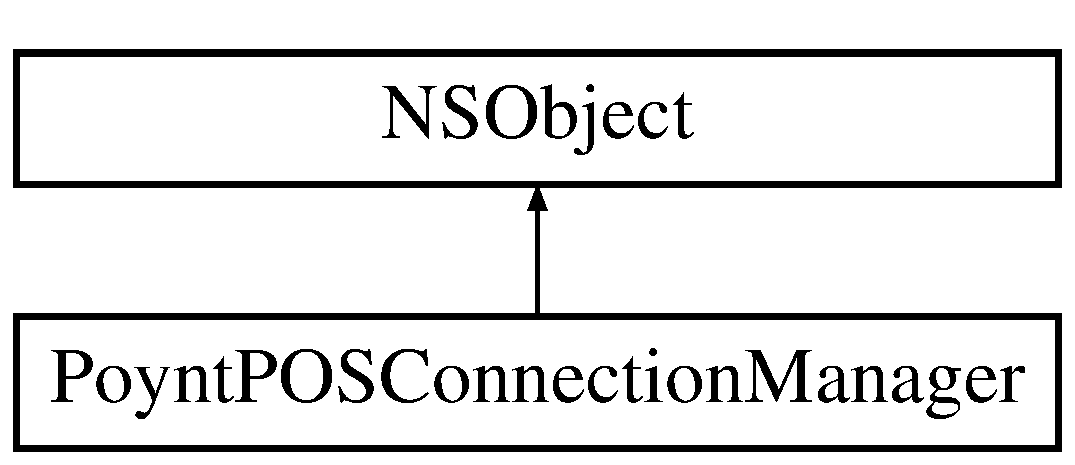
\includegraphics[height=2.000000cm]{interface_poynt_p_o_s_connection_manager}
\end{center}
\end{figure}
\subsection*{Instance Methods}
\begin{DoxyCompactItemize}
\item 
(void) -\/ \hyperlink{interface_poynt_p_o_s_connection_manager_aa35b8ab75b2115f27c8363465b2f4c85}{authorize\+Capture\+:}
\begin{DoxyCompactList}\small\item\em sends a captured sale request to the Poynt terminal \end{DoxyCompactList}\item 
(void) -\/ \hyperlink{interface_poynt_p_o_s_connection_manager_a80bcfbd9a0d3d99af46027edee12d5ba}{authorize\+Pairing\+:}
\begin{DoxyCompactList}\small\item\em attempts to pair the i\+OS client with the Poynt terminal \end{DoxyCompactList}\item 
(void) -\/ \hyperlink{interface_poynt_p_o_s_connection_manager_a9ddd4dfbae869bf65611b03472140b8e}{authorize\+Partial\+Completion\+:}
\begin{DoxyCompactList}\small\item\em sends a captured sale request to the Poynt terminal \end{DoxyCompactList}\item 
(void) -\/ \hyperlink{interface_poynt_p_o_s_connection_manager_a165211f19736758772a4427902bdb932}{authorize\+Partial\+Refund\+:}
\begin{DoxyCompactList}\small\item\em sends a partial refund request to the Poynt terminal \end{DoxyCompactList}\item 
(void) -\/ \hyperlink{interface_poynt_p_o_s_connection_manager_a3eb595755dc0ecbf9fa358f55117f021}{authorize\+Pre\+Sales\+:}
\begin{DoxyCompactList}\small\item\em sends an auth\+Only sale request to the Poynt terminal \end{DoxyCompactList}\item 
(void) -\/ \hyperlink{interface_poynt_p_o_s_connection_manager_a06494ca11a35277bc19c86dcfd34c8a4}{authorize\+Refund\+:}
\begin{DoxyCompactList}\small\item\em sends a refund request to the Poynt terminals \end{DoxyCompactList}\item 
(void) -\/ \hyperlink{interface_poynt_p_o_s_connection_manager_addc8717b201139753094f0d5d9038ea9}{authorize\+Sales\+:}
\begin{DoxyCompactList}\small\item\em sends a sale request for capture to the Poynt terminal \end{DoxyCompactList}\item 
(void) -\/ \hyperlink{interface_poynt_p_o_s_connection_manager_ac78262b676405ba3826f79c55c488e1f}{authorize\+Void\+:}
\begin{DoxyCompactList}\small\item\em sends a void request to the Poynt terminals \end{DoxyCompactList}\item 
(void) -\/ \hyperlink{interface_poynt_p_o_s_connection_manager_a9dbf19579902ee4c67310a2d705381b9}{authorize\+Void\+Pre\+Sales\+:}
\begin{DoxyCompactList}\small\item\em sends a void request to the Poynt terminals \end{DoxyCompactList}\item 
(void) -\/ \hyperlink{interface_poynt_p_o_s_connection_manager_a5a35b99719ec02d91ec102d75a49bd7a}{authorize\+Adjustment\+:}
\begin{DoxyCompactList}\small\item\em sends an adjustment request to the Poynt terminal \end{DoxyCompactList}\end{DoxyCompactItemize}
\subsection*{Properties}
\begin{DoxyCompactItemize}
\item 
N\+S\+String $\ast$ \hyperlink{interface_poynt_p_o_s_connection_manager_acc1c5e037cbbc59cd1b00f131660efe2}{client\+Name}
\begin{DoxyCompactList}\small\item\em optional property for displaying/references a name for the device implementing the Poynt\+Lib S\+DK \end{DoxyCompactList}\item 
N\+S\+String $\ast$ \hyperlink{interface_poynt_p_o_s_connection_manager_afb57bf61e0a6b264b5f2765f09a96d2b}{pairing\+Code}
\begin{DoxyCompactList}\small\item\em required property for pairing an i\+OS client with the Poynt terminal \end{DoxyCompactList}\item 
N\+S\+String $\ast$ \hyperlink{interface_poynt_p_o_s_connection_manager_a43481294fa1d2f0ebe7cff14b17726cc}{url}
\begin{DoxyCompactList}\small\item\em required property for pairing an i\+OS client with the Poynt terminal \end{DoxyCompactList}\item 
N\+S\+Integer \hyperlink{interface_poynt_p_o_s_connection_manager_ad4ac67644bd591b45e7e45448681872d}{timeout}
\begin{DoxyCompactList}\small\item\em optional property for setting the timeout for \hyperlink{interface_poynt_p_o_s_connection_manager}{Poynt\+P\+O\+S\+Connection\+Manager} requests. \end{DoxyCompactList}\item 
\hyperlink{_poynt_p_o_s_connection_manager_8h_af6bc4a828ea6541e27d04eef1263513b}{Poynt\+P\+O\+S\+Pairing\+Status} \hyperlink{interface_poynt_p_o_s_connection_manager_ac623b382557bedf15142de86ee6e2782}{pairing\+Status}
\begin{DoxyCompactList}\small\item\em readonly property for understanding the current pairing state of the \hyperlink{interface_poynt_p_o_s_connection_manager}{Poynt\+P\+O\+S\+Connection\+Manager} \end{DoxyCompactList}\item 
\hyperlink{_poynt_p_o_s_connection_manager_8h_ae268209596a83d1d61f8ce4f2513d800}{On\+Transaction\+Response} \hyperlink{interface_poynt_p_o_s_connection_manager_aec722c6cb0f961265852a406242c430b}{on\+Transaction\+Response}
\begin{DoxyCompactList}\small\item\em use the On\+Transaction\+Response block to capture the response from the Poynt terminal after a successful request completes \end{DoxyCompactList}\item 
\hyperlink{_poynt_p_o_s_connection_manager_8h_aef7c4526c1bcdb84233ca3d7f7074d5a}{On\+Error} \hyperlink{interface_poynt_p_o_s_connection_manager_a2ea439a383295e69bc2094a614e3b6fb}{on\+Error}
\begin{DoxyCompactList}\small\item\em use the On\+Error block to capture the fail state response from the Poynt terminal in the event of an error \end{DoxyCompactList}\end{DoxyCompactItemize}


\subsection{Detailed Description}
The connection manager is the gateway class to communicating with the Poynt terminal.  This object handles all things from pairing to transaction / payment specific requests 

Definition at line 43 of file Poynt\+P\+O\+S\+Connection\+Manager.\+h.



\subsection{Method Documentation}
\hypertarget{interface_poynt_p_o_s_connection_manager_a5a35b99719ec02d91ec102d75a49bd7a}{}\label{interface_poynt_p_o_s_connection_manager_a5a35b99719ec02d91ec102d75a49bd7a} 
\index{Poynt\+P\+O\+S\+Connection\+Manager@{Poynt\+P\+O\+S\+Connection\+Manager}!authorize\+Adjustment\+:@{authorize\+Adjustment\+:}}
\index{authorize\+Adjustment\+:@{authorize\+Adjustment\+:}!Poynt\+P\+O\+S\+Connection\+Manager@{Poynt\+P\+O\+S\+Connection\+Manager}}
\subsubsection{\texorpdfstring{authorize\+Adjustment\+:()}{authorizeAdjustment:()}}
{\footnotesize\ttfamily -\/ (void) authorize\+Adjustment\+: \begin{DoxyParamCaption}\item[{(\hyperlink{interface_poynt_payment_object}{Poynt\+Payment\+Object} $\ast$)}]{payment }\end{DoxyParamCaption}}



sends an adjustment request to the Poynt terminal 

This expects a \hyperlink{interface_poynt_payment_object}{Poynt\+Payment\+Object}. Upon terminal response the payment\+Manager will receive either the on\+Transaction\+Response or on\+Error handler. The payment object must have an amount associated, and optional tip\+Amount (if a tip is included)


\begin{DoxyParams}{Parameters}
{\em \hyperlink{interface_poynt_payment_object}{Poynt\+Payment\+Object}} & \\
\hline
\end{DoxyParams}
\hypertarget{interface_poynt_p_o_s_connection_manager_aa35b8ab75b2115f27c8363465b2f4c85}{}\label{interface_poynt_p_o_s_connection_manager_aa35b8ab75b2115f27c8363465b2f4c85} 
\index{Poynt\+P\+O\+S\+Connection\+Manager@{Poynt\+P\+O\+S\+Connection\+Manager}!authorize\+Capture\+:@{authorize\+Capture\+:}}
\index{authorize\+Capture\+:@{authorize\+Capture\+:}!Poynt\+P\+O\+S\+Connection\+Manager@{Poynt\+P\+O\+S\+Connection\+Manager}}
\subsubsection{\texorpdfstring{authorize\+Capture\+:()}{authorizeCapture:()}}
{\footnotesize\ttfamily -\/ (void) authorize\+Capture\+: \begin{DoxyParamCaption}\item[{(\hyperlink{interface_poynt_transaction_object}{Poynt\+Transaction\+Object} $\ast$)}]{transaction }\end{DoxyParamCaption}}



sends a captured sale request to the Poynt terminal 

This expects a valid \hyperlink{interface_poynt_transaction_object}{Poynt\+Transaction\+Object}. Upon terminal response the payment\+Manager will receive either the on\+Transaction\+Response or on\+Error handler


\begin{DoxyParams}{Parameters}
{\em \hyperlink{interface_poynt_transaction_object}{Poynt\+Transaction\+Object}} & -\/ transaction\+Id is required \\
\hline
\end{DoxyParams}
\hypertarget{interface_poynt_p_o_s_connection_manager_a80bcfbd9a0d3d99af46027edee12d5ba}{}\label{interface_poynt_p_o_s_connection_manager_a80bcfbd9a0d3d99af46027edee12d5ba} 
\index{Poynt\+P\+O\+S\+Connection\+Manager@{Poynt\+P\+O\+S\+Connection\+Manager}!authorize\+Pairing\+:@{authorize\+Pairing\+:}}
\index{authorize\+Pairing\+:@{authorize\+Pairing\+:}!Poynt\+P\+O\+S\+Connection\+Manager@{Poynt\+P\+O\+S\+Connection\+Manager}}
\subsubsection{\texorpdfstring{authorize\+Pairing\+:()}{authorizePairing:()}}
{\footnotesize\ttfamily -\/ (void) authorize\+Pairing\+: \begin{DoxyParamCaption}\item[{(N\+S\+String $\ast$)}]{code }\end{DoxyParamCaption}}



attempts to pair the i\+OS client with the Poynt terminal 

An i\+OS client creates a pair after establishing a correct url and pairing code to make the request. The \hyperlink{interface_poynt_terminal_discover}{Poynt\+Terminal\+Discover} object can find terminals on the same network, revelaing their ip address, or you can manually address the ip if you already know it. The Poynt\+Lib S\+DK will try to re-\/establish a connection with the last set credentials even after application termination. Upon terminal response the payment\+Manager will receive either the on\+Transaction\+Response or on\+Error handler


\begin{DoxyCode}
\textcolor{keyword}{self}.paymentManager.url = \textcolor{stringliteral}{@"10.0.1.23:55555"};
\textcolor{keyword}{self}.paymentManager.clientName = \textcolor{stringliteral}{@"Happy iPad"};
[\textcolor{keyword}{self}.paymentManager authorizePairing:\textcolor{keyword}{self}.textFieldCode.text];
\end{DoxyCode}



\begin{DoxyParams}{Parameters}
{\em string} & representing the pairing code \\
\hline
\end{DoxyParams}
\hypertarget{interface_poynt_p_o_s_connection_manager_a9ddd4dfbae869bf65611b03472140b8e}{}\label{interface_poynt_p_o_s_connection_manager_a9ddd4dfbae869bf65611b03472140b8e} 
\index{Poynt\+P\+O\+S\+Connection\+Manager@{Poynt\+P\+O\+S\+Connection\+Manager}!authorize\+Partial\+Completion\+:@{authorize\+Partial\+Completion\+:}}
\index{authorize\+Partial\+Completion\+:@{authorize\+Partial\+Completion\+:}!Poynt\+P\+O\+S\+Connection\+Manager@{Poynt\+P\+O\+S\+Connection\+Manager}}
\subsubsection{\texorpdfstring{authorize\+Partial\+Completion\+:()}{authorizePartialCompletion:()}}
{\footnotesize\ttfamily -\/ (void) authorize\+Partial\+Completion\+: \begin{DoxyParamCaption}\item[{(\hyperlink{interface_poynt_payment_object}{Poynt\+Payment\+Object} $\ast$)}]{payment }\end{DoxyParamCaption}}



sends a captured sale request to the Poynt terminal 

This expects a valid \hyperlink{interface_poynt_payment_object}{Poynt\+Payment\+Object}. Upon terminal response the payment\+Manager will receive either the on\+Transaction\+Response or on\+Error handler


\begin{DoxyParams}{Parameters}
{\em \hyperlink{interface_poynt_payment_object}{Poynt\+Payment\+Object}} & (where transaction\+Id is required) \\
\hline
\end{DoxyParams}
\hypertarget{interface_poynt_p_o_s_connection_manager_a165211f19736758772a4427902bdb932}{}\label{interface_poynt_p_o_s_connection_manager_a165211f19736758772a4427902bdb932} 
\index{Poynt\+P\+O\+S\+Connection\+Manager@{Poynt\+P\+O\+S\+Connection\+Manager}!authorize\+Partial\+Refund\+:@{authorize\+Partial\+Refund\+:}}
\index{authorize\+Partial\+Refund\+:@{authorize\+Partial\+Refund\+:}!Poynt\+P\+O\+S\+Connection\+Manager@{Poynt\+P\+O\+S\+Connection\+Manager}}
\subsubsection{\texorpdfstring{authorize\+Partial\+Refund\+:()}{authorizePartialRefund:()}}
{\footnotesize\ttfamily -\/ (void) authorize\+Partial\+Refund\+: \begin{DoxyParamCaption}\item[{(\hyperlink{interface_poynt_payment_object}{Poynt\+Payment\+Object} $\ast$)}]{payment }\end{DoxyParamCaption}}



sends a partial refund request to the Poynt terminal 

This expects a valid \hyperlink{interface_poynt_payment_object}{Poynt\+Payment\+Object}. Upon terminal response the payment\+Manager will receive either the on\+Transaction\+Response or on\+Error handler


\begin{DoxyParams}{Parameters}
{\em \hyperlink{interface_poynt_payment_object}{Poynt\+Payment\+Object}} & (where transaction\+Id is required) \\
\hline
\end{DoxyParams}
\hypertarget{interface_poynt_p_o_s_connection_manager_a3eb595755dc0ecbf9fa358f55117f021}{}\label{interface_poynt_p_o_s_connection_manager_a3eb595755dc0ecbf9fa358f55117f021} 
\index{Poynt\+P\+O\+S\+Connection\+Manager@{Poynt\+P\+O\+S\+Connection\+Manager}!authorize\+Pre\+Sales\+:@{authorize\+Pre\+Sales\+:}}
\index{authorize\+Pre\+Sales\+:@{authorize\+Pre\+Sales\+:}!Poynt\+P\+O\+S\+Connection\+Manager@{Poynt\+P\+O\+S\+Connection\+Manager}}
\subsubsection{\texorpdfstring{authorize\+Pre\+Sales\+:()}{authorizePreSales:()}}
{\footnotesize\ttfamily -\/ (void) authorize\+Pre\+Sales\+: \begin{DoxyParamCaption}\item[{(\hyperlink{interface_poynt_payment_object}{Poynt\+Payment\+Object} $\ast$)}]{payment }\end{DoxyParamCaption}}



sends an auth\+Only sale request to the Poynt terminal 

This expects a \hyperlink{interface_poynt_payment_object}{Poynt\+Payment\+Object}. Upon terminal response the payment\+Manager will receive either the on\+Transaction\+Response or on\+Error handler


\begin{DoxyParams}{Parameters}
{\em \hyperlink{interface_poynt_payment_object}{Poynt\+Payment\+Object}} & \\
\hline
\end{DoxyParams}
\hypertarget{interface_poynt_p_o_s_connection_manager_a06494ca11a35277bc19c86dcfd34c8a4}{}\label{interface_poynt_p_o_s_connection_manager_a06494ca11a35277bc19c86dcfd34c8a4} 
\index{Poynt\+P\+O\+S\+Connection\+Manager@{Poynt\+P\+O\+S\+Connection\+Manager}!authorize\+Refund\+:@{authorize\+Refund\+:}}
\index{authorize\+Refund\+:@{authorize\+Refund\+:}!Poynt\+P\+O\+S\+Connection\+Manager@{Poynt\+P\+O\+S\+Connection\+Manager}}
\subsubsection{\texorpdfstring{authorize\+Refund\+:()}{authorizeRefund:()}}
{\footnotesize\ttfamily -\/ (void) authorize\+Refund\+: \begin{DoxyParamCaption}\item[{(id$<$ Poynt\+Transaction $>$)}]{transaction }\end{DoxyParamCaption}}



sends a refund request to the Poynt terminals 

This method expects a valid object subscribing to the \hyperlink{class_poynt_transaction-p}{Poynt\+Transaction} protocol. The transaction\+Id must be in reference of a valid transaction. Upon terminal response the payment\+Manager will receive either the on\+Transaction\+Response or on\+Error handler


\begin{DoxyParams}{Parameters}
{\em an} & object that subscribes to the \hyperlink{class_poynt_transaction-p}{Poynt\+Transaction} protocol -\/ transaction\+Id is required \\
\hline
\end{DoxyParams}
\hypertarget{interface_poynt_p_o_s_connection_manager_addc8717b201139753094f0d5d9038ea9}{}\label{interface_poynt_p_o_s_connection_manager_addc8717b201139753094f0d5d9038ea9} 
\index{Poynt\+P\+O\+S\+Connection\+Manager@{Poynt\+P\+O\+S\+Connection\+Manager}!authorize\+Sales\+:@{authorize\+Sales\+:}}
\index{authorize\+Sales\+:@{authorize\+Sales\+:}!Poynt\+P\+O\+S\+Connection\+Manager@{Poynt\+P\+O\+S\+Connection\+Manager}}
\subsubsection{\texorpdfstring{authorize\+Sales\+:()}{authorizeSales:()}}
{\footnotesize\ttfamily -\/ (void) authorize\+Sales\+: \begin{DoxyParamCaption}\item[{(\hyperlink{interface_poynt_payment_object}{Poynt\+Payment\+Object} $\ast$)}]{payment }\end{DoxyParamCaption}}



sends a sale request for capture to the Poynt terminal 

This expects a \hyperlink{interface_poynt_payment_object}{Poynt\+Payment\+Object}. Upon terminal response the payment\+Manager will receive either the on\+Transaction\+Response or on\+Error handler


\begin{DoxyParams}{Parameters}
{\em \hyperlink{interface_poynt_payment_object}{Poynt\+Payment\+Object}} & \\
\hline
\end{DoxyParams}
\hypertarget{interface_poynt_p_o_s_connection_manager_ac78262b676405ba3826f79c55c488e1f}{}\label{interface_poynt_p_o_s_connection_manager_ac78262b676405ba3826f79c55c488e1f} 
\index{Poynt\+P\+O\+S\+Connection\+Manager@{Poynt\+P\+O\+S\+Connection\+Manager}!authorize\+Void\+:@{authorize\+Void\+:}}
\index{authorize\+Void\+:@{authorize\+Void\+:}!Poynt\+P\+O\+S\+Connection\+Manager@{Poynt\+P\+O\+S\+Connection\+Manager}}
\subsubsection{\texorpdfstring{authorize\+Void\+:()}{authorizeVoid:()}}
{\footnotesize\ttfamily -\/ (void) authorize\+Void\+: \begin{DoxyParamCaption}\item[{(id$<$ Poynt\+Transaction $>$)}]{transaction }\end{DoxyParamCaption}}



sends a void request to the Poynt terminals 

This method expects a valid object subscribing to the \hyperlink{class_poynt_transaction-p}{Poynt\+Transaction} protocol. The transaction\+Id must be in reference of a transaction. Upon terminal response the payment\+Manager will receive either the on\+Transaction\+Response or on\+Error handler


\begin{DoxyParams}{Parameters}
{\em an} & object that subscribes to the \hyperlink{class_poynt_transaction-p}{Poynt\+Transaction} protocol -\/ transaction\+Id is required \\
\hline
\end{DoxyParams}
\hypertarget{interface_poynt_p_o_s_connection_manager_a9dbf19579902ee4c67310a2d705381b9}{}\label{interface_poynt_p_o_s_connection_manager_a9dbf19579902ee4c67310a2d705381b9} 
\index{Poynt\+P\+O\+S\+Connection\+Manager@{Poynt\+P\+O\+S\+Connection\+Manager}!authorize\+Void\+Pre\+Sales\+:@{authorize\+Void\+Pre\+Sales\+:}}
\index{authorize\+Void\+Pre\+Sales\+:@{authorize\+Void\+Pre\+Sales\+:}!Poynt\+P\+O\+S\+Connection\+Manager@{Poynt\+P\+O\+S\+Connection\+Manager}}
\subsubsection{\texorpdfstring{authorize\+Void\+Pre\+Sales\+:()}{authorizeVoidPreSales:()}}
{\footnotesize\ttfamily -\/ (void) authorize\+Void\+Pre\+Sales\+: \begin{DoxyParamCaption}\item[{(id$<$ Poynt\+Transaction $>$)}]{transaction }\end{DoxyParamCaption}}



sends a void request to the Poynt terminals 

This method expects a valid object subscribing to the \hyperlink{class_poynt_transaction-p}{Poynt\+Transaction} protocol. The transaction\+Id must be in reference of an  transaction. Upon terminal response the payment\+Manager will receive either the on\+Transaction\+Response or on\+Error handler


\begin{DoxyParams}{Parameters}
{\em an} & object that subscribes to the \hyperlink{class_poynt_transaction-p}{Poynt\+Transaction} protocol -\/ transaction\+Id is required \\
\hline
\end{DoxyParams}


\subsection{Property Documentation}
\hypertarget{interface_poynt_p_o_s_connection_manager_acc1c5e037cbbc59cd1b00f131660efe2}{}\label{interface_poynt_p_o_s_connection_manager_acc1c5e037cbbc59cd1b00f131660efe2} 
\index{Poynt\+P\+O\+S\+Connection\+Manager@{Poynt\+P\+O\+S\+Connection\+Manager}!client\+Name@{client\+Name}}
\index{client\+Name@{client\+Name}!Poynt\+P\+O\+S\+Connection\+Manager@{Poynt\+P\+O\+S\+Connection\+Manager}}
\subsubsection{\texorpdfstring{client\+Name}{clientName}}
{\footnotesize\ttfamily -\/ (N\+S\+String$\ast$) client\+Name\hspace{0.3cm}{\ttfamily [read]}, {\ttfamily [write]}, {\ttfamily [nonatomic]}, {\ttfamily [strong]}}



optional property for displaying/references a name for the device implementing the Poynt\+Lib S\+DK 

When Poynt terminal pairs with an i\+OS client, it will display the name of the client and the pairing\+Code used to make the connection.

\begin{DoxyReturn}{Returns}
string for a human readable client name on the Poynt terminal 
\end{DoxyReturn}


Definition at line 51 of file Poynt\+P\+O\+S\+Connection\+Manager.\+h.

\hypertarget{interface_poynt_p_o_s_connection_manager_a2ea439a383295e69bc2094a614e3b6fb}{}\label{interface_poynt_p_o_s_connection_manager_a2ea439a383295e69bc2094a614e3b6fb} 
\index{Poynt\+P\+O\+S\+Connection\+Manager@{Poynt\+P\+O\+S\+Connection\+Manager}!on\+Error@{on\+Error}}
\index{on\+Error@{on\+Error}!Poynt\+P\+O\+S\+Connection\+Manager@{Poynt\+P\+O\+S\+Connection\+Manager}}
\subsubsection{\texorpdfstring{on\+Error}{onError}}
{\footnotesize\ttfamily -\/ (\hyperlink{_poynt_p_o_s_connection_manager_8h_aef7c4526c1bcdb84233ca3d7f7074d5a}{On\+Error}) on\+Error\hspace{0.3cm}{\ttfamily [read]}, {\ttfamily [write]}, {\ttfamily [atomic]}, {\ttfamily [copy]}}



use the On\+Error block to capture the fail state response from the Poynt terminal in the event of an error 

the block will contain an N\+S\+Error object and Poynt\+Action\+Type enum


\begin{DoxyCode}
[paymentManager setOnError:^void(NSError *error, \hyperlink{_poynt_p_o_s_connection_manager_8h_a9d1a2639d9b9775a21d4c181160e7af7}{PoyntActionType} actionType)\{

\}];
[paymentManager authorizeCapture:transactionObject]
\end{DoxyCode}
 

Definition at line 121 of file Poynt\+P\+O\+S\+Connection\+Manager.\+h.

\hypertarget{interface_poynt_p_o_s_connection_manager_aec722c6cb0f961265852a406242c430b}{}\label{interface_poynt_p_o_s_connection_manager_aec722c6cb0f961265852a406242c430b} 
\index{Poynt\+P\+O\+S\+Connection\+Manager@{Poynt\+P\+O\+S\+Connection\+Manager}!on\+Transaction\+Response@{on\+Transaction\+Response}}
\index{on\+Transaction\+Response@{on\+Transaction\+Response}!Poynt\+P\+O\+S\+Connection\+Manager@{Poynt\+P\+O\+S\+Connection\+Manager}}
\subsubsection{\texorpdfstring{on\+Transaction\+Response}{onTransactionResponse}}
{\footnotesize\ttfamily -\/ (\hyperlink{_poynt_p_o_s_connection_manager_8h_ae268209596a83d1d61f8ce4f2513d800}{On\+Transaction\+Response}) on\+Transaction\+Response\hspace{0.3cm}{\ttfamily [read]}, {\ttfamily [write]}, {\ttfamily [atomic]}, {\ttfamily [copy]}}



use the On\+Transaction\+Response block to capture the response from the Poynt terminal after a successful request completes 

the block will contain a \hyperlink{interface_poynt_transaction_response_object}{Poynt\+Transaction\+Response\+Object} object and Poynt\+Action\+Type enum to clarify from which method is being calledback


\begin{DoxyCode}
[paymentManager setOnTransactionResponse:^void(\hyperlink{interface_poynt_transaction_response_object}{PoyntTransactionResponseObject}
       *data,\hyperlink{_poynt_p_o_s_connection_manager_8h_a9d1a2639d9b9775a21d4c181160e7af7}{PoyntActionType} actionType)\{
   \textcolor{keywordflow}{if}(actionType == \hyperlink{_poynt_p_o_s_connection_manager_8h_a9d1a2639d9b9775a21d4c181160e7af7aadbbca3ad6fc42c73fa7c69608f0a4d7}{AuthorizePair})\{
       \textcolor{comment}{// ... handle this case}
   \}\textcolor{keywordflow}{else}\{
       NSLog(\textcolor{stringliteral}{@"success for %@"},data);
   \}
\}];
[paymentManager authorizeCapture:transactionObject]
\end{DoxyCode}
 

Definition at line 108 of file Poynt\+P\+O\+S\+Connection\+Manager.\+h.

\hypertarget{interface_poynt_p_o_s_connection_manager_afb57bf61e0a6b264b5f2765f09a96d2b}{}\label{interface_poynt_p_o_s_connection_manager_afb57bf61e0a6b264b5f2765f09a96d2b} 
\index{Poynt\+P\+O\+S\+Connection\+Manager@{Poynt\+P\+O\+S\+Connection\+Manager}!pairing\+Code@{pairing\+Code}}
\index{pairing\+Code@{pairing\+Code}!Poynt\+P\+O\+S\+Connection\+Manager@{Poynt\+P\+O\+S\+Connection\+Manager}}
\subsubsection{\texorpdfstring{pairing\+Code}{pairingCode}}
{\footnotesize\ttfamily -\/ (N\+S\+String$\ast$) pairing\+Code\hspace{0.3cm}{\ttfamily [read]}, {\ttfamily [write]}, {\ttfamily [nonatomic]}, {\ttfamily [strong]}}



required property for pairing an i\+OS client with the Poynt terminal 

Poynt terminal requires both a url and pairing\+Code to establish a connection for passing data.

\begin{DoxyReturn}{Returns}
string an alpha numeric code for pairing. 
\end{DoxyReturn}


Definition at line 59 of file Poynt\+P\+O\+S\+Connection\+Manager.\+h.

\hypertarget{interface_poynt_p_o_s_connection_manager_ac623b382557bedf15142de86ee6e2782}{}\label{interface_poynt_p_o_s_connection_manager_ac623b382557bedf15142de86ee6e2782} 
\index{Poynt\+P\+O\+S\+Connection\+Manager@{Poynt\+P\+O\+S\+Connection\+Manager}!pairing\+Status@{pairing\+Status}}
\index{pairing\+Status@{pairing\+Status}!Poynt\+P\+O\+S\+Connection\+Manager@{Poynt\+P\+O\+S\+Connection\+Manager}}
\subsubsection{\texorpdfstring{pairing\+Status}{pairingStatus}}
{\footnotesize\ttfamily -\/ (\hyperlink{_poynt_p_o_s_connection_manager_8h_af6bc4a828ea6541e27d04eef1263513b}{Poynt\+P\+O\+S\+Pairing\+Status}) pairing\+Status\hspace{0.3cm}{\ttfamily [read]}, {\ttfamily [nonatomic]}, {\ttfamily [assign]}}



readonly property for understanding the current pairing state of the \hyperlink{interface_poynt_p_o_s_connection_manager}{Poynt\+P\+O\+S\+Connection\+Manager} 

\begin{DoxyReturn}{Returns}
enum 
\end{DoxyReturn}


Definition at line 90 of file Poynt\+P\+O\+S\+Connection\+Manager.\+h.

\hypertarget{interface_poynt_p_o_s_connection_manager_ad4ac67644bd591b45e7e45448681872d}{}\label{interface_poynt_p_o_s_connection_manager_ad4ac67644bd591b45e7e45448681872d} 
\index{Poynt\+P\+O\+S\+Connection\+Manager@{Poynt\+P\+O\+S\+Connection\+Manager}!timeout@{timeout}}
\index{timeout@{timeout}!Poynt\+P\+O\+S\+Connection\+Manager@{Poynt\+P\+O\+S\+Connection\+Manager}}
\subsubsection{\texorpdfstring{timeout}{timeout}}
{\footnotesize\ttfamily -\/ (N\+S\+Integer) timeout\hspace{0.3cm}{\ttfamily [read]}, {\ttfamily [write]}, {\ttfamily [nonatomic]}, {\ttfamily [assign]}}



optional property for setting the timeout for \hyperlink{interface_poynt_p_o_s_connection_manager}{Poynt\+P\+O\+S\+Connection\+Manager} requests. 

Timout is understood in milliseconds by the Poynt terminal. The timeout can be set previous to making a request, depending on what suits best for the client application. Setting a new timeout value is persitant until reset to a new value. The default value is 60000 ( = one minute)

\begin{DoxyReturn}{Returns}
N\+S\+Integer 
\end{DoxyReturn}


Definition at line 83 of file Poynt\+P\+O\+S\+Connection\+Manager.\+h.

\hypertarget{interface_poynt_p_o_s_connection_manager_a43481294fa1d2f0ebe7cff14b17726cc}{}\label{interface_poynt_p_o_s_connection_manager_a43481294fa1d2f0ebe7cff14b17726cc} 
\index{Poynt\+P\+O\+S\+Connection\+Manager@{Poynt\+P\+O\+S\+Connection\+Manager}!url@{url}}
\index{url@{url}!Poynt\+P\+O\+S\+Connection\+Manager@{Poynt\+P\+O\+S\+Connection\+Manager}}
\subsubsection{\texorpdfstring{url}{url}}
{\footnotesize\ttfamily -\/ (N\+S\+String$\ast$) url\hspace{0.3cm}{\ttfamily [read]}, {\ttfamily [write]}, {\ttfamily [nonatomic]}, {\ttfamily [strong]}}



required property for pairing an i\+OS client with the Poynt terminal 

Poynt terminal requires both a url and pairing\+Code to establish a connection for passing data. The url can be discovered by using the \hyperlink{interface_poynt_terminal_discover}{Poynt\+Terminal\+Discover} object for discovery over Wi\+Fi

\begin{DoxyReturn}{Returns}
string for an ip address, including port if necessary.
\end{DoxyReturn}

\begin{DoxyCode}
\textcolor{keyword}{self}.paymentManager.url = \textcolor{stringliteral}{@"10.0.2.21:55555"}
\end{DoxyCode}


\begin{DoxySeeAlso}{See also}
\hyperlink{_poynt_terminal_discover_8h}{Poynt\+Terminal\+Discover.\+h} 
\end{DoxySeeAlso}


Definition at line 74 of file Poynt\+P\+O\+S\+Connection\+Manager.\+h.



The documentation for this class was generated from the following file\+:\begin{DoxyCompactItemize}
\item 
Poynt\+Lib/\hyperlink{_poynt_p_o_s_connection_manager_8h}{Poynt\+P\+O\+S\+Connection\+Manager.\+h}\end{DoxyCompactItemize}

\hypertarget{interface_poynt_terminal}{}\section{Poynt\+Terminal Class Reference}
\label{interface_poynt_terminal}\index{Poynt\+Terminal@{Poynt\+Terminal}}


{\ttfamily \#import $<$Poynt\+Terminal.\+h$>$}

Inheritance diagram for Poynt\+Terminal\+:\begin{figure}[H]
\begin{center}
\leavevmode
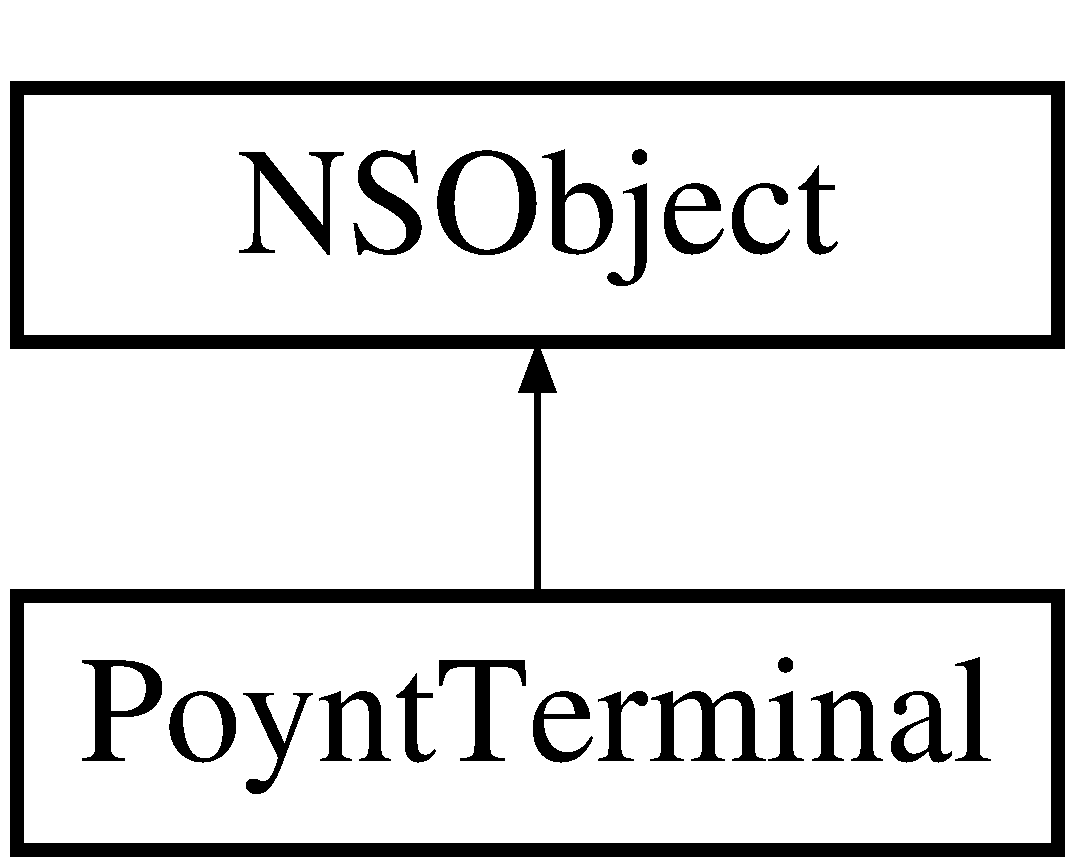
\includegraphics[height=2.000000cm]{interface_poynt_terminal}
\end{center}
\end{figure}
\subsection*{Instance Methods}
\begin{DoxyCompactItemize}
\item 
(id) -\/ \hyperlink{interface_poynt_terminal_a85d039f4fe918b4ab91b90c1bac883f1}{init\+With\+Service\+:}
\begin{DoxyCompactList}\small\item\em only use init\+With\+Service to create a \hyperlink{interface_poynt_terminal}{Poynt\+Terminal} object \end{DoxyCompactList}\end{DoxyCompactItemize}
\subsection*{Properties}
\begin{DoxyCompactItemize}
\item 
N\+S\+String $\ast$ \hyperlink{interface_poynt_terminal_a4b93d352d2fca75b34e1b5a50e03f587}{name}
\begin{DoxyCompactList}\small\item\em the name of the terminal \end{DoxyCompactList}\item 
N\+S\+String $\ast$ \hyperlink{interface_poynt_terminal_ab18eca4fc399814b2e86f54006b1e474}{ip}
\begin{DoxyCompactList}\small\item\em the ip of the terminal  In the event the terminal identifies an explicit port for pairing, it will be found here \end{DoxyCompactList}\item 
N\+S\+U\+RL $\ast$ \hyperlink{interface_poynt_terminal_a8d02094b967129e59efcc8c670677184}{url}
\begin{DoxyCompactList}\small\item\em the url object for connecting with this terminal \end{DoxyCompactList}\item 
N\+S\+Net\+Service $\ast$ \hyperlink{interface_poynt_terminal_a4c12c4a257de1f39c44a0a72b272246a}{service}
\begin{DoxyCompactList}\small\item\em Poynt\+Lib S\+DK utilized bonjour over W\+I\+FI to detect terminals. The service object is engaged when we reach for pairing the device to client  Use \hyperlink{interface_poynt_terminal_discover}{Poynt\+Terminal\+Discover} to find the service. \end{DoxyCompactList}\end{DoxyCompactItemize}


\subsection{Detailed Description}
\hyperlink{interface_poynt_terminal}{Poynt\+Terminal}  objects are useful during the terminal discovery phase when on the same W\+I\+FI network. It is entirey possible to connect manually to a terminal without using a \hyperlink{interface_poynt_terminal}{Poynt\+Terminal} object, as long as the ip address and connection code is known. \begin{DoxySeeAlso}{See also}
\hyperlink{interface_poynt_p_o_s_connection_manager}{Poynt\+P\+O\+S\+Connection\+Manager}
\end{DoxySeeAlso}
\begin{DoxyRefDesc}{Todo}
\item[\hyperlink{todo__todo000001}{Todo}]allow multiple terminal connections. Currently, only one terminal connection is supported \end{DoxyRefDesc}


Definition at line 17 of file Poynt\+Terminal.\+h.



\subsection{Method Documentation}
\hypertarget{interface_poynt_terminal_a85d039f4fe918b4ab91b90c1bac883f1}{}\label{interface_poynt_terminal_a85d039f4fe918b4ab91b90c1bac883f1} 
\index{Poynt\+Terminal@{Poynt\+Terminal}!init\+With\+Service\+:@{init\+With\+Service\+:}}
\index{init\+With\+Service\+:@{init\+With\+Service\+:}!Poynt\+Terminal@{Poynt\+Terminal}}
\subsubsection{\texorpdfstring{init\+With\+Service\+:()}{initWithService:()}}
{\footnotesize\ttfamily -\/ (id) init\+With\+Service\+: \begin{DoxyParamCaption}\item[{(N\+S\+Net\+Service $\ast$)}]{service }\end{DoxyParamCaption}}



only use init\+With\+Service to create a \hyperlink{interface_poynt_terminal}{Poynt\+Terminal} object 



\subsection{Property Documentation}
\hypertarget{interface_poynt_terminal_ab18eca4fc399814b2e86f54006b1e474}{}\label{interface_poynt_terminal_ab18eca4fc399814b2e86f54006b1e474} 
\index{Poynt\+Terminal@{Poynt\+Terminal}!ip@{ip}}
\index{ip@{ip}!Poynt\+Terminal@{Poynt\+Terminal}}
\subsubsection{\texorpdfstring{ip}{ip}}
{\footnotesize\ttfamily -\/ (N\+S\+String$\ast$) ip\hspace{0.3cm}{\ttfamily [read]}, {\ttfamily [write]}, {\ttfamily [nonatomic]}, {\ttfamily [strong]}}



the ip of the terminal  In the event the terminal identifies an explicit port for pairing, it will be found here 



Definition at line 26 of file Poynt\+Terminal.\+h.

\hypertarget{interface_poynt_terminal_a4b93d352d2fca75b34e1b5a50e03f587}{}\label{interface_poynt_terminal_a4b93d352d2fca75b34e1b5a50e03f587} 
\index{Poynt\+Terminal@{Poynt\+Terminal}!name@{name}}
\index{name@{name}!Poynt\+Terminal@{Poynt\+Terminal}}
\subsubsection{\texorpdfstring{name}{name}}
{\footnotesize\ttfamily -\/ (N\+S\+String$\ast$) name\hspace{0.3cm}{\ttfamily [read]}, {\ttfamily [write]}, {\ttfamily [nonatomic]}, {\ttfamily [strong]}}



the name of the terminal 



Definition at line 21 of file Poynt\+Terminal.\+h.

\hypertarget{interface_poynt_terminal_a4c12c4a257de1f39c44a0a72b272246a}{}\label{interface_poynt_terminal_a4c12c4a257de1f39c44a0a72b272246a} 
\index{Poynt\+Terminal@{Poynt\+Terminal}!service@{service}}
\index{service@{service}!Poynt\+Terminal@{Poynt\+Terminal}}
\subsubsection{\texorpdfstring{service}{service}}
{\footnotesize\ttfamily -\/ (N\+S\+Net\+Service$\ast$) service\hspace{0.3cm}{\ttfamily [read]}, {\ttfamily [write]}, {\ttfamily [nonatomic]}, {\ttfamily [strong]}}



Poynt\+Lib S\+DK utilized bonjour over W\+I\+FI to detect terminals. The service object is engaged when we reach for pairing the device to client  Use \hyperlink{interface_poynt_terminal_discover}{Poynt\+Terminal\+Discover} to find the service. 



Definition at line 35 of file Poynt\+Terminal.\+h.

\hypertarget{interface_poynt_terminal_a8d02094b967129e59efcc8c670677184}{}\label{interface_poynt_terminal_a8d02094b967129e59efcc8c670677184} 
\index{Poynt\+Terminal@{Poynt\+Terminal}!url@{url}}
\index{url@{url}!Poynt\+Terminal@{Poynt\+Terminal}}
\subsubsection{\texorpdfstring{url}{url}}
{\footnotesize\ttfamily -\/ (N\+S\+U\+RL$\ast$) url\hspace{0.3cm}{\ttfamily [read]}, {\ttfamily [write]}, {\ttfamily [nonatomic]}, {\ttfamily [strong]}}



the url object for connecting with this terminal 



Definition at line 30 of file Poynt\+Terminal.\+h.



The documentation for this class was generated from the following file\+:\begin{DoxyCompactItemize}
\item 
Poynt\+Lib/models/\hyperlink{_poynt_terminal_8h}{Poynt\+Terminal.\+h}\end{DoxyCompactItemize}

\hypertarget{interface_poynt_terminal_discover}{}\section{Poynt\+Terminal\+Discover Class Reference}
\label{interface_poynt_terminal_discover}\index{Poynt\+Terminal\+Discover@{Poynt\+Terminal\+Discover}}


{\ttfamily \#import $<$Poynt\+Terminal\+Discover.\+h$>$}

Inheritance diagram for Poynt\+Terminal\+Discover\+:\begin{figure}[H]
\begin{center}
\leavevmode
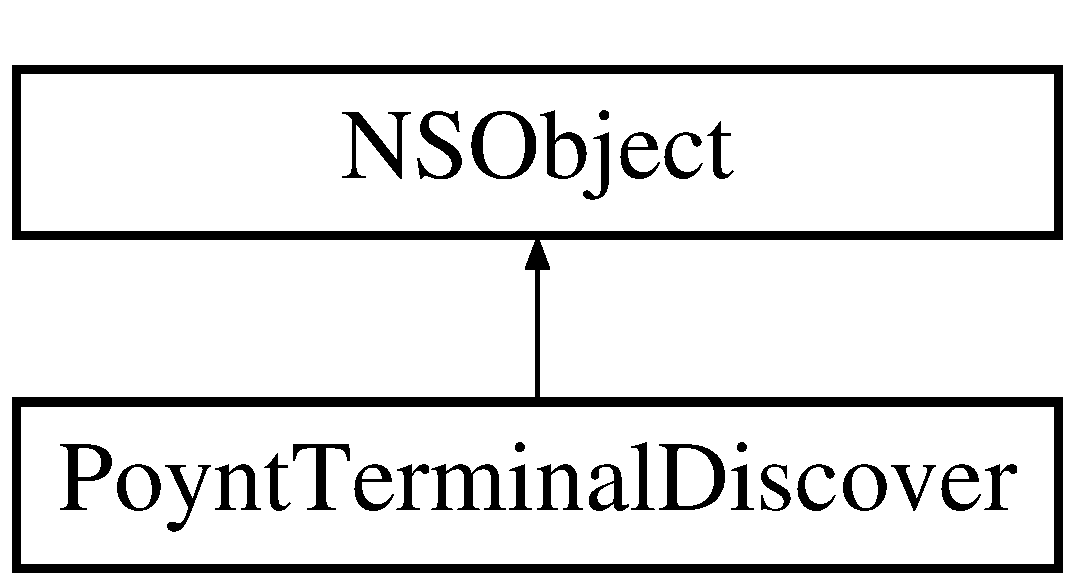
\includegraphics[height=2.000000cm]{interface_poynt_terminal_discover}
\end{center}
\end{figure}
\subsection*{Instance Methods}
\begin{DoxyCompactItemize}
\item 
(void) -\/ \hyperlink{interface_poynt_terminal_discover_aab8fdef29321b4bf9ff4ba57e1593e9a}{find\+Terminals\+:}
\begin{DoxyCompactList}\small\item\em find terminals on the same W\+I\+FI network  pass an On\+Terminals\+Found block to get a list of terminals currently known on the network. \end{DoxyCompactList}\end{DoxyCompactItemize}
\subsection*{Properties}
\begin{DoxyCompactItemize}
\item 
N\+S\+Array $\ast$ \hyperlink{interface_poynt_terminal_discover_a5388c2786127d007a5b553986779ee46}{terminals}
\begin{DoxyCompactList}\small\item\em list of \hyperlink{interface_poynt_terminal}{Poynt\+Terminal} currently known on the network \end{DoxyCompactList}\item 
\hyperlink{_poynt_terminal_discover_8h_a45c48a836064cd340f281fa5ef2edef5}{On\+Terminals\+Found} \hyperlink{interface_poynt_terminal_discover_a2108a121006de9953dbf24fa265db472}{on\+Terminals\+Found}
\begin{DoxyCompactList}\small\item\em callback called upon finding the device(s) on the W\+I\+FI.  This callback is called only one time. If you need to refresh the search, you must call find\+Terminals\+:complete again \end{DoxyCompactList}\item 
B\+O\+OL \hyperlink{interface_poynt_terminal_discover_a3ec4dc196847dee68ad6c99d08bfef95}{searching}
\begin{DoxyCompactList}\small\item\em Boolean value decalaring if the object is searching or is done searching. \end{DoxyCompactList}\end{DoxyCompactItemize}


\subsection{Detailed Description}


Definition at line 19 of file Poynt\+Terminal\+Discover.\+h.



\subsection{Method Documentation}
\hypertarget{interface_poynt_terminal_discover_aab8fdef29321b4bf9ff4ba57e1593e9a}{}\label{interface_poynt_terminal_discover_aab8fdef29321b4bf9ff4ba57e1593e9a} 
\index{Poynt\+Terminal\+Discover@{Poynt\+Terminal\+Discover}!find\+Terminals\+:@{find\+Terminals\+:}}
\index{find\+Terminals\+:@{find\+Terminals\+:}!Poynt\+Terminal\+Discover@{Poynt\+Terminal\+Discover}}
\subsubsection{\texorpdfstring{find\+Terminals\+:()}{findTerminals:()}}
{\footnotesize\ttfamily -\/ (void) find\+Terminals\+: \begin{DoxyParamCaption}\item[{(\hyperlink{_poynt_terminal_discover_8h_a45c48a836064cd340f281fa5ef2edef5}{On\+Terminals\+Found})}]{complete }\end{DoxyParamCaption}}



find terminals on the same W\+I\+FI network  pass an On\+Terminals\+Found block to get a list of terminals currently known on the network. 



\subsection{Property Documentation}
\hypertarget{interface_poynt_terminal_discover_a2108a121006de9953dbf24fa265db472}{}\label{interface_poynt_terminal_discover_a2108a121006de9953dbf24fa265db472} 
\index{Poynt\+Terminal\+Discover@{Poynt\+Terminal\+Discover}!on\+Terminals\+Found@{on\+Terminals\+Found}}
\index{on\+Terminals\+Found@{on\+Terminals\+Found}!Poynt\+Terminal\+Discover@{Poynt\+Terminal\+Discover}}
\subsubsection{\texorpdfstring{on\+Terminals\+Found}{onTerminalsFound}}
{\footnotesize\ttfamily -\/ (\hyperlink{_poynt_terminal_discover_8h_a45c48a836064cd340f281fa5ef2edef5}{On\+Terminals\+Found}) on\+Terminals\+Found\hspace{0.3cm}{\ttfamily [read]}, {\ttfamily [write]}, {\ttfamily [nonatomic]}, {\ttfamily [copy]}}



callback called upon finding the device(s) on the W\+I\+FI.  This callback is called only one time. If you need to refresh the search, you must call find\+Terminals\+:complete again 



Definition at line 28 of file Poynt\+Terminal\+Discover.\+h.

\hypertarget{interface_poynt_terminal_discover_a3ec4dc196847dee68ad6c99d08bfef95}{}\label{interface_poynt_terminal_discover_a3ec4dc196847dee68ad6c99d08bfef95} 
\index{Poynt\+Terminal\+Discover@{Poynt\+Terminal\+Discover}!searching@{searching}}
\index{searching@{searching}!Poynt\+Terminal\+Discover@{Poynt\+Terminal\+Discover}}
\subsubsection{\texorpdfstring{searching}{searching}}
{\footnotesize\ttfamily -\/ (B\+O\+OL) searching\hspace{0.3cm}{\ttfamily [read]}, {\ttfamily [write]}, {\ttfamily [nonatomic]}, {\ttfamily [assign]}}



Boolean value decalaring if the object is searching or is done searching. 



Definition at line 32 of file Poynt\+Terminal\+Discover.\+h.

\hypertarget{interface_poynt_terminal_discover_a5388c2786127d007a5b553986779ee46}{}\label{interface_poynt_terminal_discover_a5388c2786127d007a5b553986779ee46} 
\index{Poynt\+Terminal\+Discover@{Poynt\+Terminal\+Discover}!terminals@{terminals}}
\index{terminals@{terminals}!Poynt\+Terminal\+Discover@{Poynt\+Terminal\+Discover}}
\subsubsection{\texorpdfstring{terminals}{terminals}}
{\footnotesize\ttfamily -\/ (N\+S\+Array$\ast$) terminals\hspace{0.3cm}{\ttfamily [read]}, {\ttfamily [write]}, {\ttfamily [nonatomic]}, {\ttfamily [strong]}}



list of \hyperlink{interface_poynt_terminal}{Poynt\+Terminal} currently known on the network 



Definition at line 23 of file Poynt\+Terminal\+Discover.\+h.



The documentation for this class was generated from the following file\+:\begin{DoxyCompactItemize}
\item 
Poynt\+Lib/\hyperlink{_poynt_terminal_discover_8h}{Poynt\+Terminal\+Discover.\+h}\end{DoxyCompactItemize}

\hypertarget{protocol_poynt_transaction_01-p}{}\section{$<$Poynt\+Transaction $>$ Protocol Reference}
\label{protocol_poynt_transaction_01-p}\index{$<$\+Poynt\+Transaction $>$@{$<$\+Poynt\+Transaction $>$}}


When in doubt (or lazy) default to a \hyperlink{interface_poynt_transaction_object}{Poynt\+Transaction\+Object}. In cases where it is optimal to keep clear seperation, subscribe to \hyperlink{class_poynt_transaction-p}{Poynt\+Transaction} . The transaction\+Id property and dictionary\+Object method are required.  




{\ttfamily \#import $<$Poynt\+Transaction.\+h$>$}

Inheritance diagram for $<$Poynt\+Transaction $>$\+:\begin{figure}[H]
\begin{center}
\leavevmode
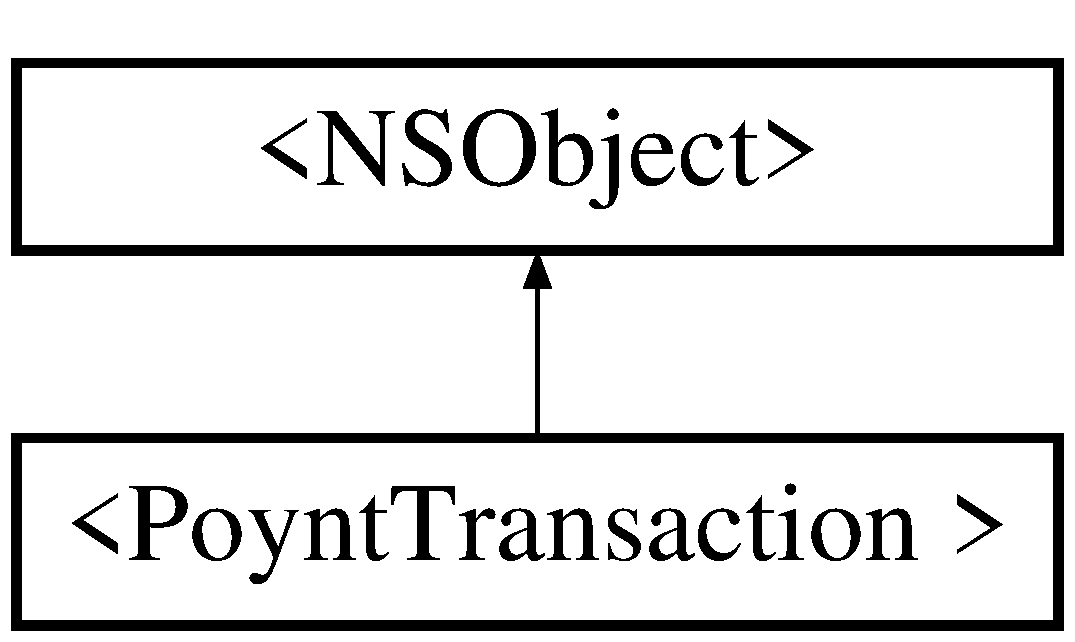
\includegraphics[height=2.000000cm]{protocol_poynt_transaction_01-p}
\end{center}
\end{figure}
\subsection*{Instance Methods}
\begin{DoxyCompactItemize}
\item 
(N\+S\+Dictionary $\ast$) -\/ \hyperlink{protocol_poynt_transaction_01-p_a2482f2e9af7fe8eec4ba9710cdc963ee}{dictionary\+Object}
\begin{DoxyCompactList}\small\item\em dictionary representation of this object \end{DoxyCompactList}\end{DoxyCompactItemize}
\subsection*{Properties}
\begin{DoxyCompactItemize}
\item 
N\+S\+String $\ast$ \hyperlink{protocol_poynt_transaction_01-p_aacd11580c330a78310c344d78baecf8c}{transaction\+Id}
\begin{DoxyCompactList}\small\item\em required property representing a transaction\+Id from past terminal requests, or a new transaction\+Id for creating transaction (eg sale or pre\+Sale) \end{DoxyCompactList}\end{DoxyCompactItemize}


\subsection{Detailed Description}
When in doubt (or lazy) default to a \hyperlink{interface_poynt_transaction_object}{Poynt\+Transaction\+Object}. In cases where it is optimal to keep clear seperation, subscribe to \hyperlink{class_poynt_transaction-p}{Poynt\+Transaction} . The transaction\+Id property and dictionary\+Object method are required. 

\hyperlink{_poynt_transaction_8h}{Poynt\+Transaction.\+h} 

Definition at line 17 of file Poynt\+Transaction.\+h.



\subsection{Method Documentation}
\hypertarget{protocol_poynt_transaction_01-p_a2482f2e9af7fe8eec4ba9710cdc963ee}{}\label{protocol_poynt_transaction_01-p_a2482f2e9af7fe8eec4ba9710cdc963ee} 
\index{Poynt\+Transaction -\/p@{Poynt\+Transaction -\/p}!dictionary\+Object@{dictionary\+Object}}
\index{dictionary\+Object@{dictionary\+Object}!Poynt\+Transaction -\/p@{Poynt\+Transaction -\/p}}
\subsubsection{\texorpdfstring{dictionary\+Object()}{dictionaryObject()}}
{\footnotesize\ttfamily -\/ (N\+S\+Dictionary$\ast$) dictionary\+Object \begin{DoxyParamCaption}{ }\end{DoxyParamCaption}}



dictionary representation of this object 

the dictionary object is most commonly used in cases to serialize data for making requests.

\begin{DoxyReturn}{Returns}
dictionary 
\end{DoxyReturn}


\subsection{Property Documentation}
\hypertarget{protocol_poynt_transaction_01-p_aacd11580c330a78310c344d78baecf8c}{}\label{protocol_poynt_transaction_01-p_aacd11580c330a78310c344d78baecf8c} 
\index{Poynt\+Transaction -\/p@{Poynt\+Transaction -\/p}!transaction\+Id@{transaction\+Id}}
\index{transaction\+Id@{transaction\+Id}!Poynt\+Transaction -\/p@{Poynt\+Transaction -\/p}}
\subsubsection{\texorpdfstring{transaction\+Id}{transactionId}}
{\footnotesize\ttfamily -\/ (N\+S\+String$\ast$) transaction\+Id\hspace{0.3cm}{\ttfamily [read]}, {\ttfamily [write]}, {\ttfamily [nonatomic]}, {\ttfamily [copy]}}



required property representing a transaction\+Id from past terminal requests, or a new transaction\+Id for creating transaction (eg sale or pre\+Sale) 

Poynt terminal requires both a url and pairing\+Code to establish a connection for passing data.

\begin{DoxyReturn}{Returns}
string -\/ commonly in the format of {\ttfamily }\mbox{[}\mbox{[}N\+S\+U\+U\+ID U\+U\+ID\mbox{]} U\+U\+I\+D\+String\mbox{]} 
\end{DoxyReturn}


Definition at line 26 of file Poynt\+Transaction.\+h.



The documentation for this protocol was generated from the following file\+:\begin{DoxyCompactItemize}
\item 
Poynt\+Lib/models/\hyperlink{_poynt_transaction_8h}{Poynt\+Transaction.\+h}\end{DoxyCompactItemize}

\hypertarget{interface_poynt_transaction_amounts}{}\section{Poynt\+Transaction\+Amounts Class Reference}
\label{interface_poynt_transaction_amounts}\index{Poynt\+Transaction\+Amounts@{Poynt\+Transaction\+Amounts}}


the transaction amounts in a \hyperlink{interface_poynt_transaction_object}{Poynt\+Transaction\+Object} amounts collection  




{\ttfamily \#import $<$Poynt\+Transaction\+Amounts.\+h$>$}

Inheritance diagram for Poynt\+Transaction\+Amounts\+:\begin{figure}[H]
\begin{center}
\leavevmode
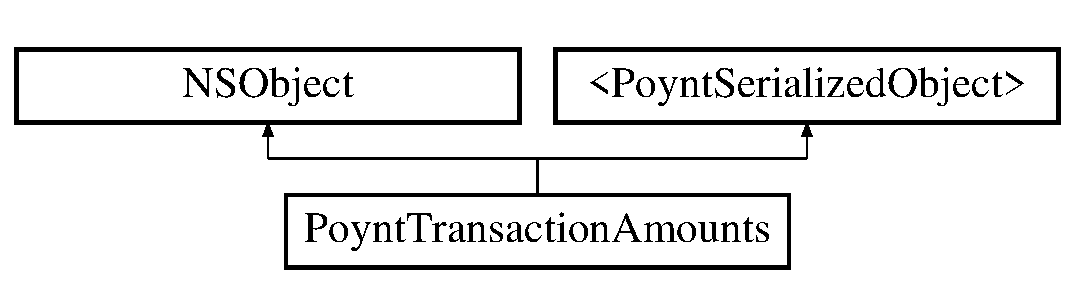
\includegraphics[height=2.000000cm]{interface_poynt_transaction_amounts}
\end{center}
\end{figure}
\subsection*{Instance Methods}
\begin{DoxyCompactItemize}
\item 
(id) -\/ \hyperlink{interface_poynt_transaction_amounts_af1bc93b54ea2b50650a15f84ced4f921}{init\+With\+Amount\+:tip\+Amount\+:cashback\+Amount\+:}
\begin{DoxyCompactList}\small\item\em sets the order amount, tip amount, and cashback amount at initialization \end{DoxyCompactList}\item 
(id) -\/ \hyperlink{interface_poynt_transaction_amounts_ac4a96ce3f50982e0f88ef099c2b3dc5b}{init\+With\+Data\+:}
\begin{DoxyCompactList}\small\item\em creates a transaction amount with an appropriate dictionary representation \end{DoxyCompactList}\item 
(void) -\/ \hyperlink{interface_poynt_transaction_amounts_a1c43473c035627846e64fddfb2bbe57d}{calculate\+:}
\begin{DoxyCompactList}\small\item\em called on an order object to update the properties attached to this object \end{DoxyCompactList}\end{DoxyCompactItemize}
\subsection*{Properties}
\begin{DoxyCompactItemize}
\item 
N\+S\+Integer \hyperlink{interface_poynt_transaction_amounts_a37e598d8b46c97a36f7fbb47e7b150ad}{order\+Amount}
\begin{DoxyCompactList}\small\item\em required field representing amount  The portion of transaction\+Amount that went towards the item/service being purchased. \end{DoxyCompactList}\item 
N\+S\+Integer \hyperlink{interface_poynt_transaction_amounts_ae4a2e64d79032bc8bb25305486b23859}{tip\+Amount}
\item 
N\+S\+Integer \hyperlink{interface_poynt_transaction_amounts_a865d904d3a3af78f51b64d9acd5d2076}{cashback\+Amount}
\item 
N\+S\+Integer \hyperlink{interface_poynt_transaction_amounts_aea3b857ebe452c1822cdd05e35cd2769}{transaction\+Amount}
\begin{DoxyCompactList}\small\item\em required amount field  The total amount to be charged on the tender. This equals order\+Amount + tip\+Amount + cashback\+Amount. \end{DoxyCompactList}\item 
N\+S\+String $\ast$ \hyperlink{interface_poynt_transaction_amounts_a71a9104f71558df8791cedc5e81941a3}{currency}
\end{DoxyCompactItemize}


\subsection{Detailed Description}
the transaction amounts in a \hyperlink{interface_poynt_transaction_object}{Poynt\+Transaction\+Object} amounts collection 

\hyperlink{interface_poynt_transaction_amounts}{Poynt\+Transaction\+Amounts} 

Definition at line 17 of file Poynt\+Transaction\+Amounts.\+h.



\subsection{Method Documentation}
\hypertarget{interface_poynt_transaction_amounts_a1c43473c035627846e64fddfb2bbe57d}{}\label{interface_poynt_transaction_amounts_a1c43473c035627846e64fddfb2bbe57d} 
\index{Poynt\+Transaction\+Amounts@{Poynt\+Transaction\+Amounts}!calculate\+:@{calculate\+:}}
\index{calculate\+:@{calculate\+:}!Poynt\+Transaction\+Amounts@{Poynt\+Transaction\+Amounts}}
\subsubsection{\texorpdfstring{calculate\+:()}{calculate:()}}
{\footnotesize\ttfamily -\/ (void) calculate\+: \begin{DoxyParamCaption}\item[{(\hyperlink{interface_poynt_order_object}{Poynt\+Order\+Object} $\ast$)}]{order }\end{DoxyParamCaption}}



called on an order object to update the properties attached to this object 

\hypertarget{interface_poynt_transaction_amounts_af1bc93b54ea2b50650a15f84ced4f921}{}\label{interface_poynt_transaction_amounts_af1bc93b54ea2b50650a15f84ced4f921} 
\index{Poynt\+Transaction\+Amounts@{Poynt\+Transaction\+Amounts}!init\+With\+Amount\+:tip\+Amount\+:cashback\+Amount\+:@{init\+With\+Amount\+:tip\+Amount\+:cashback\+Amount\+:}}
\index{init\+With\+Amount\+:tip\+Amount\+:cashback\+Amount\+:@{init\+With\+Amount\+:tip\+Amount\+:cashback\+Amount\+:}!Poynt\+Transaction\+Amounts@{Poynt\+Transaction\+Amounts}}
\subsubsection{\texorpdfstring{init\+With\+Amount\+:tip\+Amount\+:cashback\+Amount\+:()}{initWithAmount:tipAmount:cashbackAmount:()}}
{\footnotesize\ttfamily -\/ (id) init\+With\+Amount\+: \begin{DoxyParamCaption}\item[{(N\+S\+Integer)}]{order\+Amount }\item[{tipAmount:(N\+S\+Integer)}]{tip\+Amount }\item[{cashbackAmount:(N\+S\+Integer)}]{cashback\+Amount }\end{DoxyParamCaption}}



sets the order amount, tip amount, and cashback amount at initialization 

\hypertarget{interface_poynt_transaction_amounts_ac4a96ce3f50982e0f88ef099c2b3dc5b}{}\label{interface_poynt_transaction_amounts_ac4a96ce3f50982e0f88ef099c2b3dc5b} 
\index{Poynt\+Transaction\+Amounts@{Poynt\+Transaction\+Amounts}!init\+With\+Data\+:@{init\+With\+Data\+:}}
\index{init\+With\+Data\+:@{init\+With\+Data\+:}!Poynt\+Transaction\+Amounts@{Poynt\+Transaction\+Amounts}}
\subsubsection{\texorpdfstring{init\+With\+Data\+:()}{initWithData:()}}
{\footnotesize\ttfamily -\/ (id) init\+With\+Data\+: \begin{DoxyParamCaption}\item[{(N\+S\+Dictionary $\ast$)}]{data }\end{DoxyParamCaption}}



creates a transaction amount with an appropriate dictionary representation 



\subsection{Property Documentation}
\hypertarget{interface_poynt_transaction_amounts_a865d904d3a3af78f51b64d9acd5d2076}{}\label{interface_poynt_transaction_amounts_a865d904d3a3af78f51b64d9acd5d2076} 
\index{Poynt\+Transaction\+Amounts@{Poynt\+Transaction\+Amounts}!cashback\+Amount@{cashback\+Amount}}
\index{cashback\+Amount@{cashback\+Amount}!Poynt\+Transaction\+Amounts@{Poynt\+Transaction\+Amounts}}
\subsubsection{\texorpdfstring{cashback\+Amount}{cashbackAmount}}
{\footnotesize\ttfamily -\/ (N\+S\+Integer) cashback\+Amount\hspace{0.3cm}{\ttfamily [read]}, {\ttfamily [write]}, {\ttfamily [nonatomic]}, {\ttfamily [assign]}}

The portion of transaction\+Amount that will be returned as cashback (mainly applicable for cash or debit-\/card tenders). Defaults to 0 if not provided. 

Definition at line 30 of file Poynt\+Transaction\+Amounts.\+h.

\hypertarget{interface_poynt_transaction_amounts_a71a9104f71558df8791cedc5e81941a3}{}\label{interface_poynt_transaction_amounts_a71a9104f71558df8791cedc5e81941a3} 
\index{Poynt\+Transaction\+Amounts@{Poynt\+Transaction\+Amounts}!currency@{currency}}
\index{currency@{currency}!Poynt\+Transaction\+Amounts@{Poynt\+Transaction\+Amounts}}
\subsubsection{\texorpdfstring{currency}{currency}}
{\footnotesize\ttfamily -\/ (N\+S\+String$\ast$) currency\hspace{0.3cm}{\ttfamily [read]}, {\ttfamily [write]}, {\ttfamily [nonatomic]}, {\ttfamily [strong]}}

Currency following the I\+S\+O-\/4217 format (\href{http://en.wikipedia.org/wiki/ISO_4217}{\tt http\+://en.\+wikipedia.\+org/wiki/\+I\+S\+O\+\_\+4217}). 

Definition at line 39 of file Poynt\+Transaction\+Amounts.\+h.

\hypertarget{interface_poynt_transaction_amounts_a37e598d8b46c97a36f7fbb47e7b150ad}{}\label{interface_poynt_transaction_amounts_a37e598d8b46c97a36f7fbb47e7b150ad} 
\index{Poynt\+Transaction\+Amounts@{Poynt\+Transaction\+Amounts}!order\+Amount@{order\+Amount}}
\index{order\+Amount@{order\+Amount}!Poynt\+Transaction\+Amounts@{Poynt\+Transaction\+Amounts}}
\subsubsection{\texorpdfstring{order\+Amount}{orderAmount}}
{\footnotesize\ttfamily -\/ (N\+S\+Integer) order\+Amount\hspace{0.3cm}{\ttfamily [read]}, {\ttfamily [write]}, {\ttfamily [nonatomic]}, {\ttfamily [assign]}}



required field representing amount  The portion of transaction\+Amount that went towards the item/service being purchased. 



Definition at line 22 of file Poynt\+Transaction\+Amounts.\+h.

\hypertarget{interface_poynt_transaction_amounts_ae4a2e64d79032bc8bb25305486b23859}{}\label{interface_poynt_transaction_amounts_ae4a2e64d79032bc8bb25305486b23859} 
\index{Poynt\+Transaction\+Amounts@{Poynt\+Transaction\+Amounts}!tip\+Amount@{tip\+Amount}}
\index{tip\+Amount@{tip\+Amount}!Poynt\+Transaction\+Amounts@{Poynt\+Transaction\+Amounts}}
\subsubsection{\texorpdfstring{tip\+Amount}{tipAmount}}
{\footnotesize\ttfamily -\/ (N\+S\+Integer) tip\+Amount\hspace{0.3cm}{\ttfamily [read]}, {\ttfamily [write]}, {\ttfamily [nonatomic]}, {\ttfamily [assign]}}

The portion of transaction\+Amount that went towards tip. Defaults to 0 if not provided. 

Definition at line 26 of file Poynt\+Transaction\+Amounts.\+h.

\hypertarget{interface_poynt_transaction_amounts_aea3b857ebe452c1822cdd05e35cd2769}{}\label{interface_poynt_transaction_amounts_aea3b857ebe452c1822cdd05e35cd2769} 
\index{Poynt\+Transaction\+Amounts@{Poynt\+Transaction\+Amounts}!transaction\+Amount@{transaction\+Amount}}
\index{transaction\+Amount@{transaction\+Amount}!Poynt\+Transaction\+Amounts@{Poynt\+Transaction\+Amounts}}
\subsubsection{\texorpdfstring{transaction\+Amount}{transactionAmount}}
{\footnotesize\ttfamily -\/ (N\+S\+Integer) transaction\+Amount\hspace{0.3cm}{\ttfamily [read]}, {\ttfamily [write]}, {\ttfamily [nonatomic]}, {\ttfamily [assign]}}



required amount field  The total amount to be charged on the tender. This equals order\+Amount + tip\+Amount + cashback\+Amount. 



Definition at line 35 of file Poynt\+Transaction\+Amounts.\+h.



The documentation for this class was generated from the following file\+:\begin{DoxyCompactItemize}
\item 
Poynt\+Lib/models/\hyperlink{_poynt_transaction_amounts_8h}{Poynt\+Transaction\+Amounts.\+h}\end{DoxyCompactItemize}

\hypertarget{interface_poynt_transaction_object}{}\section{Poynt\+Transaction\+Object Class Reference}
\label{interface_poynt_transaction_object}\index{Poynt\+Transaction\+Object@{Poynt\+Transaction\+Object}}


{\ttfamily \#import $<$Poynt\+Transaction\+Object.\+h$>$}

Inheritance diagram for Poynt\+Transaction\+Object\+:\begin{figure}[H]
\begin{center}
\leavevmode
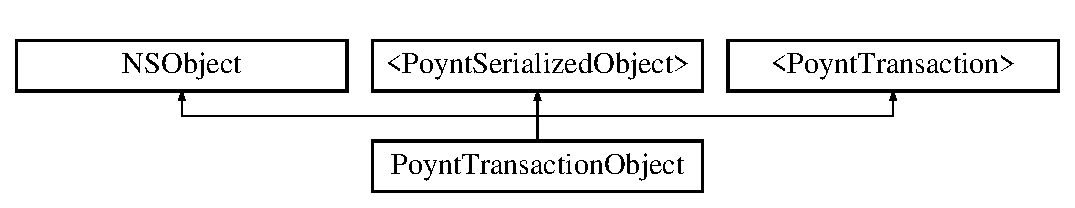
\includegraphics[height=2.000000cm]{interface_poynt_transaction_object}
\end{center}
\end{figure}
\subsection*{Instance Methods}
\begin{DoxyCompactItemize}
\item 
(id) -\/ \hyperlink{interface_poynt_transaction_object_a777cf6da1ae0fc9452b06142a5adaa14}{init\+With\+Dictionary\+:}
\begin{DoxyCompactList}\small\item\em create a \hyperlink{interface_poynt_transaction_object}{Poynt\+Transaction\+Object} using an appropriate formated dictionary object \end{DoxyCompactList}\end{DoxyCompactItemize}
\subsection*{Properties}
\begin{DoxyCompactItemize}
\item 
N\+S\+String $\ast$ \hyperlink{interface_poynt_transaction_object_af3bd537ec19ed3fac0b5aa56812a1577}{poynt\+Request\+Id}
\begin{DoxyCompactList}\small\item\em U\+U\+I\+D\+String representing this object. \end{DoxyCompactList}\item 
N\+S\+String $\ast$ \hyperlink{interface_poynt_transaction_object_aacd11580c330a78310c344d78baecf8c}{transaction\+Id}
\begin{DoxyCompactList}\small\item\em U\+U\+I\+D\+String representing a Poynt transaction id. \end{DoxyCompactList}\item 
N\+S\+String $\ast$ \hyperlink{interface_poynt_transaction_object_ac2acf327011ce6ed9e26a41ceddaee31}{status}
\begin{DoxyCompactList}\small\item\em current status of this object. Mostly commonly set server side\+: \textquotesingle{}C\+R\+E\+A\+T\+ED\textquotesingle{}, \textquotesingle{}S\+A\+V\+ED\textquotesingle{}, \textquotesingle{}A\+U\+T\+H\+O\+R\+I\+Z\+ED\textquotesingle{}, \textquotesingle{}P\+A\+R\+T\+I\+A\+L\+L\+Y\+\_\+\+C\+A\+P\+T\+U\+R\+ED\textquotesingle{}, \textquotesingle{}C\+A\+P\+T\+U\+R\+ED\textquotesingle{}, \textquotesingle{}D\+E\+C\+L\+I\+N\+ED\textquotesingle{}, \textquotesingle{}P\+A\+R\+T\+I\+A\+L\+L\+Y\+\_\+\+C\+A\+P\+T\+U\+R\+E\+D\+\_\+\+A\+N\+D\+\_\+\+P\+A\+R\+T\+I\+A\+L\+L\+Y\+\_\+\+R\+E\+F\+U\+N\+D\+ED\textquotesingle{}, \textquotesingle{}P\+A\+R\+T\+I\+A\+L\+L\+Y\+\_\+\+R\+E\+F\+U\+N\+D\+ED\textquotesingle{}, \textquotesingle{}R\+E\+F\+U\+N\+D\+ED\textquotesingle{}, \textquotesingle{}V\+O\+I\+D\+ED\textquotesingle{} \end{DoxyCompactList}\item 
N\+S\+String $\ast$ \hyperlink{interface_poynt_transaction_object_aaab84b2e5d0ad0f648e7e0e17c6afa08}{action}
\begin{DoxyCompactList}\small\item\em action of this object  \textquotesingle{}A\+U\+T\+H\+O\+R\+I\+ZE\textquotesingle{}, \textquotesingle{}C\+A\+P\+T\+U\+RE\textquotesingle{}, \textquotesingle{}O\+F\+F\+L\+I\+N\+E\+\_\+\+A\+U\+T\+H\+O\+R\+I\+ZE\textquotesingle{}, \textquotesingle{}R\+E\+F\+U\+ND\textquotesingle{}, \textquotesingle{}S\+A\+LE\textquotesingle{}, most commonly set by server \end{DoxyCompactList}\item 
N\+S\+Array $\ast$ \hyperlink{interface_poynt_transaction_object_a5ab449d070271ee2c9d138bb7b472a6c}{amounts}
\begin{DoxyCompactList}\small\item\em collection of \hyperlink{interface_poynt_transaction_amounts}{Poynt\+Transaction\+Amounts} objects \end{DoxyCompactList}\item 
N\+S\+Array $\ast$ \hyperlink{interface_poynt_transaction_object_ab4cac3360e86d21570d89915c99e6943}{funding\+Source}
\begin{DoxyCompactList}\small\item\em collection of funding source objects used for funding this transaction. \end{DoxyCompactList}\item 
N\+S\+Dictionary $\ast$ \hyperlink{interface_poynt_transaction_object_a97674af3143e04f09bbc6590dab812d7}{context}
\begin{DoxyCompactList}\small\item\em Contains context about the transaction. \end{DoxyCompactList}\item 
N\+S\+Dictionary $\ast$ \hyperlink{interface_poynt_transaction_object_a2bdc3d5a4da018a352f33b946a0ea384}{references}
\begin{DoxyCompactList}\small\item\em References to orders/invoices that this transaction is for. \end{DoxyCompactList}\end{DoxyCompactItemize}


\subsection{Detailed Description}
\hyperlink{interface_poynt_transaction_object}{Poynt\+Transaction\+Object} 

Definition at line 16 of file Poynt\+Transaction\+Object.\+h.



\subsection{Method Documentation}
\hypertarget{interface_poynt_transaction_object_a777cf6da1ae0fc9452b06142a5adaa14}{}\label{interface_poynt_transaction_object_a777cf6da1ae0fc9452b06142a5adaa14} 
\index{Poynt\+Transaction\+Object@{Poynt\+Transaction\+Object}!init\+With\+Dictionary\+:@{init\+With\+Dictionary\+:}}
\index{init\+With\+Dictionary\+:@{init\+With\+Dictionary\+:}!Poynt\+Transaction\+Object@{Poynt\+Transaction\+Object}}
\subsubsection{\texorpdfstring{init\+With\+Dictionary\+:()}{initWithDictionary:()}}
{\footnotesize\ttfamily -\/ (id) init\+With\+Dictionary\+: \begin{DoxyParamCaption}\item[{(N\+S\+Dictionary $\ast$)}]{data }\end{DoxyParamCaption}}



create a \hyperlink{interface_poynt_transaction_object}{Poynt\+Transaction\+Object} using an appropriate formated dictionary object 



\subsection{Property Documentation}
\hypertarget{interface_poynt_transaction_object_aaab84b2e5d0ad0f648e7e0e17c6afa08}{}\label{interface_poynt_transaction_object_aaab84b2e5d0ad0f648e7e0e17c6afa08} 
\index{Poynt\+Transaction\+Object@{Poynt\+Transaction\+Object}!action@{action}}
\index{action@{action}!Poynt\+Transaction\+Object@{Poynt\+Transaction\+Object}}
\subsubsection{\texorpdfstring{action}{action}}
{\footnotesize\ttfamily -\/ (N\+S\+String$\ast$) action\hspace{0.3cm}{\ttfamily [read]}, {\ttfamily [write]}, {\ttfamily [nonatomic]}, {\ttfamily [copy]}}



action of this object  \textquotesingle{}A\+U\+T\+H\+O\+R\+I\+ZE\textquotesingle{}, \textquotesingle{}C\+A\+P\+T\+U\+RE\textquotesingle{}, \textquotesingle{}O\+F\+F\+L\+I\+N\+E\+\_\+\+A\+U\+T\+H\+O\+R\+I\+ZE\textquotesingle{}, \textquotesingle{}R\+E\+F\+U\+ND\textquotesingle{}, \textquotesingle{}S\+A\+LE\textquotesingle{}, most commonly set by server 



Definition at line 33 of file Poynt\+Transaction\+Object.\+h.

\hypertarget{interface_poynt_transaction_object_a5ab449d070271ee2c9d138bb7b472a6c}{}\label{interface_poynt_transaction_object_a5ab449d070271ee2c9d138bb7b472a6c} 
\index{Poynt\+Transaction\+Object@{Poynt\+Transaction\+Object}!amounts@{amounts}}
\index{amounts@{amounts}!Poynt\+Transaction\+Object@{Poynt\+Transaction\+Object}}
\subsubsection{\texorpdfstring{amounts}{amounts}}
{\footnotesize\ttfamily -\/ (N\+S\+Array$\ast$) amounts\hspace{0.3cm}{\ttfamily [read]}, {\ttfamily [write]}, {\ttfamily [nonatomic]}, {\ttfamily [strong]}}



collection of \hyperlink{interface_poynt_transaction_amounts}{Poynt\+Transaction\+Amounts} objects 



Definition at line 37 of file Poynt\+Transaction\+Object.\+h.

\hypertarget{interface_poynt_transaction_object_a97674af3143e04f09bbc6590dab812d7}{}\label{interface_poynt_transaction_object_a97674af3143e04f09bbc6590dab812d7} 
\index{Poynt\+Transaction\+Object@{Poynt\+Transaction\+Object}!context@{context}}
\index{context@{context}!Poynt\+Transaction\+Object@{Poynt\+Transaction\+Object}}
\subsubsection{\texorpdfstring{context}{context}}
{\footnotesize\ttfamily -\/ (N\+S\+Dictionary$\ast$) context\hspace{0.3cm}{\ttfamily [read]}, {\ttfamily [write]}, {\ttfamily [nonatomic]}, {\ttfamily [strong]}}



Contains context about the transaction. 



Definition at line 46 of file Poynt\+Transaction\+Object.\+h.

\hypertarget{interface_poynt_transaction_object_ab4cac3360e86d21570d89915c99e6943}{}\label{interface_poynt_transaction_object_ab4cac3360e86d21570d89915c99e6943} 
\index{Poynt\+Transaction\+Object@{Poynt\+Transaction\+Object}!funding\+Source@{funding\+Source}}
\index{funding\+Source@{funding\+Source}!Poynt\+Transaction\+Object@{Poynt\+Transaction\+Object}}
\subsubsection{\texorpdfstring{funding\+Source}{fundingSource}}
{\footnotesize\ttfamily -\/ (N\+S\+Array$\ast$) funding\+Source\hspace{0.3cm}{\ttfamily [read]}, {\ttfamily [write]}, {\ttfamily [nonatomic]}, {\ttfamily [strong]}}



collection of funding source objects used for funding this transaction. 

\begin{DoxyRefDesc}{Todo}
\item[\hyperlink{todo__todo000002}{Todo}]at current, we are not populating this field. Developers have access to the data in \hyperlink{interface_poynt_transaction_response_object_a0046f618ca04fd1e7fcf91b87190a944}{Poynt\+Transaction\+Response\+Object.\+raw\+Json} propety \end{DoxyRefDesc}


Definition at line 42 of file Poynt\+Transaction\+Object.\+h.

\hypertarget{interface_poynt_transaction_object_af3bd537ec19ed3fac0b5aa56812a1577}{}\label{interface_poynt_transaction_object_af3bd537ec19ed3fac0b5aa56812a1577} 
\index{Poynt\+Transaction\+Object@{Poynt\+Transaction\+Object}!poynt\+Request\+Id@{poynt\+Request\+Id}}
\index{poynt\+Request\+Id@{poynt\+Request\+Id}!Poynt\+Transaction\+Object@{Poynt\+Transaction\+Object}}
\subsubsection{\texorpdfstring{poynt\+Request\+Id}{poyntRequestId}}
{\footnotesize\ttfamily -\/ (N\+S\+String$\ast$) poynt\+Request\+Id\hspace{0.3cm}{\ttfamily [read]}, {\ttfamily [write]}, {\ttfamily [nonatomic]}, {\ttfamily [copy]}}



U\+U\+I\+D\+String representing this object. 



Definition at line 20 of file Poynt\+Transaction\+Object.\+h.

\hypertarget{interface_poynt_transaction_object_a2bdc3d5a4da018a352f33b946a0ea384}{}\label{interface_poynt_transaction_object_a2bdc3d5a4da018a352f33b946a0ea384} 
\index{Poynt\+Transaction\+Object@{Poynt\+Transaction\+Object}!references@{references}}
\index{references@{references}!Poynt\+Transaction\+Object@{Poynt\+Transaction\+Object}}
\subsubsection{\texorpdfstring{references}{references}}
{\footnotesize\ttfamily -\/ (N\+S\+Dictionary$\ast$) references\hspace{0.3cm}{\ttfamily [read]}, {\ttfamily [write]}, {\ttfamily [nonatomic]}, {\ttfamily [strong]}}



References to orders/invoices that this transaction is for. 



Definition at line 50 of file Poynt\+Transaction\+Object.\+h.

\hypertarget{interface_poynt_transaction_object_ac2acf327011ce6ed9e26a41ceddaee31}{}\label{interface_poynt_transaction_object_ac2acf327011ce6ed9e26a41ceddaee31} 
\index{Poynt\+Transaction\+Object@{Poynt\+Transaction\+Object}!status@{status}}
\index{status@{status}!Poynt\+Transaction\+Object@{Poynt\+Transaction\+Object}}
\subsubsection{\texorpdfstring{status}{status}}
{\footnotesize\ttfamily -\/ (N\+S\+String$\ast$) status\hspace{0.3cm}{\ttfamily [read]}, {\ttfamily [write]}, {\ttfamily [nonatomic]}, {\ttfamily [copy]}}



current status of this object. Mostly commonly set server side\+: \textquotesingle{}C\+R\+E\+A\+T\+ED\textquotesingle{}, \textquotesingle{}S\+A\+V\+ED\textquotesingle{}, \textquotesingle{}A\+U\+T\+H\+O\+R\+I\+Z\+ED\textquotesingle{}, \textquotesingle{}P\+A\+R\+T\+I\+A\+L\+L\+Y\+\_\+\+C\+A\+P\+T\+U\+R\+ED\textquotesingle{}, \textquotesingle{}C\+A\+P\+T\+U\+R\+ED\textquotesingle{}, \textquotesingle{}D\+E\+C\+L\+I\+N\+ED\textquotesingle{}, \textquotesingle{}P\+A\+R\+T\+I\+A\+L\+L\+Y\+\_\+\+C\+A\+P\+T\+U\+R\+E\+D\+\_\+\+A\+N\+D\+\_\+\+P\+A\+R\+T\+I\+A\+L\+L\+Y\+\_\+\+R\+E\+F\+U\+N\+D\+ED\textquotesingle{}, \textquotesingle{}P\+A\+R\+T\+I\+A\+L\+L\+Y\+\_\+\+R\+E\+F\+U\+N\+D\+ED\textquotesingle{}, \textquotesingle{}R\+E\+F\+U\+N\+D\+ED\textquotesingle{}, \textquotesingle{}V\+O\+I\+D\+ED\textquotesingle{} 



Definition at line 28 of file Poynt\+Transaction\+Object.\+h.

\hypertarget{interface_poynt_transaction_object_aacd11580c330a78310c344d78baecf8c}{}\label{interface_poynt_transaction_object_aacd11580c330a78310c344d78baecf8c} 
\index{Poynt\+Transaction\+Object@{Poynt\+Transaction\+Object}!transaction\+Id@{transaction\+Id}}
\index{transaction\+Id@{transaction\+Id}!Poynt\+Transaction\+Object@{Poynt\+Transaction\+Object}}
\subsubsection{\texorpdfstring{transaction\+Id}{transactionId}}
{\footnotesize\ttfamily -\/ (N\+S\+String$\ast$) transaction\+Id\hspace{0.3cm}{\ttfamily [read]}, {\ttfamily [write]}, {\ttfamily [nonatomic]}, {\ttfamily [copy]}}



U\+U\+I\+D\+String representing a Poynt transaction id. 



Definition at line 24 of file Poynt\+Transaction\+Object.\+h.



The documentation for this class was generated from the following file\+:\begin{DoxyCompactItemize}
\item 
Poynt\+Lib/models/\hyperlink{_poynt_transaction_object_8h}{Poynt\+Transaction\+Object.\+h}\end{DoxyCompactItemize}

\hypertarget{interface_poynt_transaction_response_object}{}\section{Poynt\+Transaction\+Response\+Object Class Reference}
\label{interface_poynt_transaction_response_object}\index{Poynt\+Transaction\+Response\+Object@{Poynt\+Transaction\+Response\+Object}}


A \hyperlink{interface_poynt_transaction_response_object}{Poynt\+Transaction\+Response\+Object} is the response from a succesful terminal request. It is not a guarantee that the intended request has the results desired (see {\ttfamily response\+Error}) and can be further understood by its properties.  




{\ttfamily \#import $<$Poynt\+Transaction\+Response\+Object.\+h$>$}

Inheritance diagram for Poynt\+Transaction\+Response\+Object\+:\begin{figure}[H]
\begin{center}
\leavevmode
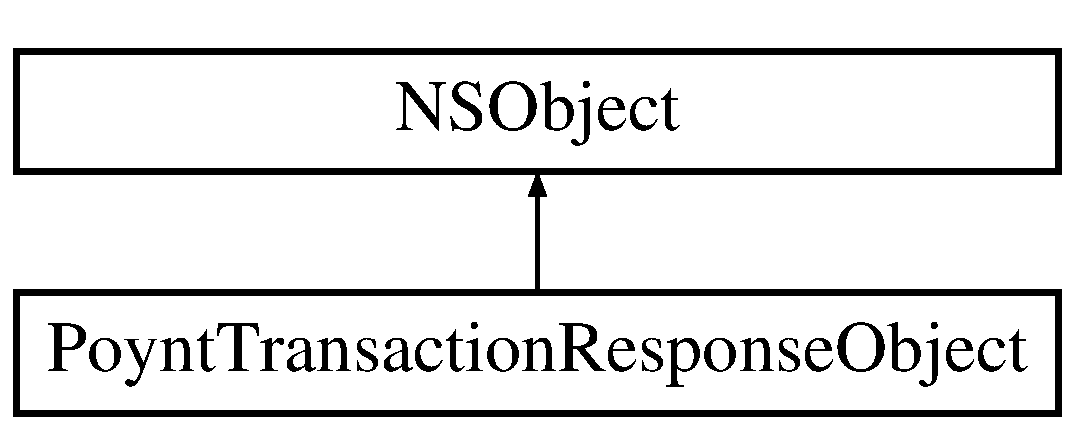
\includegraphics[height=2.000000cm]{interface_poynt_transaction_response_object}
\end{center}
\end{figure}
\subsection*{Instance Methods}
\begin{DoxyCompactItemize}
\item 
(id) -\/ \hyperlink{interface_poynt_transaction_response_object_a42ee83b8c11bd68e673b38d2a96ca170}{init\+With\+Data\+:}
\end{DoxyCompactItemize}
\subsection*{Properties}
\begin{DoxyCompactItemize}
\item 
N\+S\+Error $\ast$ \hyperlink{interface_poynt_transaction_response_object_aefb1590b30be0658ebee825cad6bfa83}{response\+Error}
\begin{DoxyCompactList}\small\item\em this field will only be populated if there was an error in the request. Most commonly, the error will be descriptive of the problem. \end{DoxyCompactList}\item 
N\+S\+String $\ast$ \hyperlink{interface_poynt_transaction_response_object_ac2acf327011ce6ed9e26a41ceddaee31}{status}
\item 
N\+S\+Array $\ast$ \hyperlink{interface_poynt_transaction_response_object_a12474d50a1838843bcc1cacbbc30c4d2}{transactions}
\item 
N\+S\+Dictionary $\ast$ \hyperlink{interface_poynt_transaction_response_object_a14f67be3c2e0d0a1dfbaf225c2fcef4b}{order}
\item 
N\+S\+Dictionary $\ast$ \hyperlink{interface_poynt_transaction_response_object_a0046f618ca04fd1e7fcf91b87190a944}{raw\+Json}
\end{DoxyCompactItemize}


\subsection{Detailed Description}
A \hyperlink{interface_poynt_transaction_response_object}{Poynt\+Transaction\+Response\+Object} is the response from a succesful terminal request. It is not a guarantee that the intended request has the results desired (see {\ttfamily response\+Error}) and can be further understood by its properties. 

\hyperlink{interface_poynt_transaction_response_object}{Poynt\+Transaction\+Response\+Object} 

Definition at line 16 of file Poynt\+Transaction\+Response\+Object.\+h.



\subsection{Method Documentation}
\hypertarget{interface_poynt_transaction_response_object_a42ee83b8c11bd68e673b38d2a96ca170}{}\label{interface_poynt_transaction_response_object_a42ee83b8c11bd68e673b38d2a96ca170} 
\index{Poynt\+Transaction\+Response\+Object@{Poynt\+Transaction\+Response\+Object}!init\+With\+Data\+:@{init\+With\+Data\+:}}
\index{init\+With\+Data\+:@{init\+With\+Data\+:}!Poynt\+Transaction\+Response\+Object@{Poynt\+Transaction\+Response\+Object}}
\subsubsection{\texorpdfstring{init\+With\+Data\+:()}{initWithData:()}}
{\footnotesize\ttfamily -\/ (id) init\+With\+Data\+: \begin{DoxyParamCaption}\item[{(N\+S\+Data $\ast$)}]{data }\end{DoxyParamCaption}}

This initialization is generally reserved for the S\+DK , however remains exposed in the event a developer needs to create their own response object


\begin{DoxyParams}{Parameters}
{\em data} & formatted from a Poynt\+Services response \\
\hline
\end{DoxyParams}
\begin{DoxyReturn}{Returns}
a valid \hyperlink{interface_poynt_transaction_response_object}{Poynt\+Transaction\+Response\+Object} 
\end{DoxyReturn}


\subsection{Property Documentation}
\hypertarget{interface_poynt_transaction_response_object_a14f67be3c2e0d0a1dfbaf225c2fcef4b}{}\label{interface_poynt_transaction_response_object_a14f67be3c2e0d0a1dfbaf225c2fcef4b} 
\index{Poynt\+Transaction\+Response\+Object@{Poynt\+Transaction\+Response\+Object}!order@{order}}
\index{order@{order}!Poynt\+Transaction\+Response\+Object@{Poynt\+Transaction\+Response\+Object}}
\subsubsection{\texorpdfstring{order}{order}}
{\footnotesize\ttfamily -\/ (N\+S\+Dictionary$\ast$) order\hspace{0.3cm}{\ttfamily [read]}, {\ttfamily [write]}, {\ttfamily [nonatomic]}, {\ttfamily [strong]}}

dictionary representation of \hyperlink{interface_poynt_order_object}{Poynt\+Order\+Object} \begin{DoxyNote}{Note}
This is an optional field an often not dependable (ie\+: not populated) 
\end{DoxyNote}


Definition at line 36 of file Poynt\+Transaction\+Response\+Object.\+h.

\hypertarget{interface_poynt_transaction_response_object_a0046f618ca04fd1e7fcf91b87190a944}{}\label{interface_poynt_transaction_response_object_a0046f618ca04fd1e7fcf91b87190a944} 
\index{Poynt\+Transaction\+Response\+Object@{Poynt\+Transaction\+Response\+Object}!raw\+Json@{raw\+Json}}
\index{raw\+Json@{raw\+Json}!Poynt\+Transaction\+Response\+Object@{Poynt\+Transaction\+Response\+Object}}
\subsubsection{\texorpdfstring{raw\+Json}{rawJson}}
{\footnotesize\ttfamily -\/ (N\+S\+Dictionary$\ast$) raw\+Json\hspace{0.3cm}{\ttfamily [read]}, {\ttfamily [nonatomic]}, {\ttfamily [assign]}}

all \hyperlink{interface_poynt_transaction_response_object}{Poynt\+Transaction\+Response\+Object} will contain their {\ttfamily raw\+Json} which can often be useful for attaching more dynamic key/value representations of the response. It is not uncommon for objects to differ in property count or general inheritance 

Definition at line 41 of file Poynt\+Transaction\+Response\+Object.\+h.

\hypertarget{interface_poynt_transaction_response_object_aefb1590b30be0658ebee825cad6bfa83}{}\label{interface_poynt_transaction_response_object_aefb1590b30be0658ebee825cad6bfa83} 
\index{Poynt\+Transaction\+Response\+Object@{Poynt\+Transaction\+Response\+Object}!response\+Error@{response\+Error}}
\index{response\+Error@{response\+Error}!Poynt\+Transaction\+Response\+Object@{Poynt\+Transaction\+Response\+Object}}
\subsubsection{\texorpdfstring{response\+Error}{responseError}}
{\footnotesize\ttfamily -\/ (N\+S\+Error$\ast$) response\+Error\hspace{0.3cm}{\ttfamily [read]}, {\ttfamily [nonatomic]}, {\ttfamily [assign]}}



this field will only be populated if there was an error in the request. Most commonly, the error will be descriptive of the problem. 



Definition at line 21 of file Poynt\+Transaction\+Response\+Object.\+h.

\hypertarget{interface_poynt_transaction_response_object_ac2acf327011ce6ed9e26a41ceddaee31}{}\label{interface_poynt_transaction_response_object_ac2acf327011ce6ed9e26a41ceddaee31} 
\index{Poynt\+Transaction\+Response\+Object@{Poynt\+Transaction\+Response\+Object}!status@{status}}
\index{status@{status}!Poynt\+Transaction\+Response\+Object@{Poynt\+Transaction\+Response\+Object}}
\subsubsection{\texorpdfstring{status}{status}}
{\footnotesize\ttfamily -\/ (N\+S\+String$\ast$) status\hspace{0.3cm}{\ttfamily [read]}, {\ttfamily [write]}, {\ttfamily [nonatomic]}, {\ttfamily [copy]}}

if successful, will be a value of \char`\"{}\+C\+O\+M\+P\+L\+E\+T\+E\+D\char`\"{} or \char`\"{}\+S\+U\+C\+C\+E\+S\+S\char`\"{} 

Definition at line 25 of file Poynt\+Transaction\+Response\+Object.\+h.

\hypertarget{interface_poynt_transaction_response_object_a12474d50a1838843bcc1cacbbc30c4d2}{}\label{interface_poynt_transaction_response_object_a12474d50a1838843bcc1cacbbc30c4d2} 
\index{Poynt\+Transaction\+Response\+Object@{Poynt\+Transaction\+Response\+Object}!transactions@{transactions}}
\index{transactions@{transactions}!Poynt\+Transaction\+Response\+Object@{Poynt\+Transaction\+Response\+Object}}
\subsubsection{\texorpdfstring{transactions}{transactions}}
{\footnotesize\ttfamily -\/ (N\+S\+Array$\ast$) transactions\hspace{0.3cm}{\ttfamily [read]}, {\ttfamily [write]}, {\ttfamily [nonatomic]}, {\ttfamily [strong]}}

a collection of \hyperlink{interface_poynt_transaction_object}{Poynt\+Transaction\+Object} objects attached to this transaction request. 

Definition at line 30 of file Poynt\+Transaction\+Response\+Object.\+h.



The documentation for this class was generated from the following file\+:\begin{DoxyCompactItemize}
\item 
Poynt\+Lib/models/\hyperlink{_poynt_transaction_response_object_8h}{Poynt\+Transaction\+Response\+Object.\+h}\end{DoxyCompactItemize}

\chapter{File Documentation}
\hypertarget{_poynt_discount_object_8h}{}\section{Poynt\+Lib/models/\+Poynt\+Discount\+Object.h File Reference}
\label{_poynt_discount_object_8h}\index{Poynt\+Lib/models/\+Poynt\+Discount\+Object.\+h@{Poynt\+Lib/models/\+Poynt\+Discount\+Object.\+h}}
{\ttfamily \#import $<$Foundation/\+Foundation.\+h$>$}\newline
{\ttfamily \#import \char`\"{}Poynt\+Serialized\+Object.\+h\char`\"{}}\newline
\subsection*{Data Structures}
\begin{DoxyCompactItemize}
\item 
class \hyperlink{interface_poynt_discount_object}{Poynt\+Discount\+Object}
\end{DoxyCompactItemize}

\hypertarget{_poynt_order_item_object_8h}{}\section{Poynt\+Lib/models/\+Poynt\+Order\+Item\+Object.h File Reference}
\label{_poynt_order_item_object_8h}\index{Poynt\+Lib/models/\+Poynt\+Order\+Item\+Object.\+h@{Poynt\+Lib/models/\+Poynt\+Order\+Item\+Object.\+h}}
{\ttfamily \#import $<$Foundation/\+Foundation.\+h$>$}\newline
{\ttfamily \#import \char`\"{}Poynt\+Serialized\+Object.\+h\char`\"{}}\newline
\subsection*{Data Structures}
\begin{DoxyCompactItemize}
\item 
class \hyperlink{interface_poynt_order_item_object}{Poynt\+Order\+Item\+Object}
\end{DoxyCompactItemize}
\subsection*{Enumerations}
\begin{DoxyCompactItemize}
\item 
enum \hyperlink{_poynt_order_item_object_8h_a7a5dd044bd57739d1d1b3e3565fbac25}{Unit\+Of\+Measure} \{ \newline
\hyperlink{_poynt_order_item_object_8h_a7a5dd044bd57739d1d1b3e3565fbac25a230bc1794689a94bd302517282cb4e88}{E\+A\+CH}, 
\hyperlink{_poynt_order_item_object_8h_a7a5dd044bd57739d1d1b3e3565fbac25a4071f24c62fa1c9c6c34b8d2dd0f2b4e}{H\+O\+U\+RS}, 
\hyperlink{_poynt_order_item_object_8h_a7a5dd044bd57739d1d1b3e3565fbac25aecd160bcb5fa0d5e062562b01487f202}{D\+A\+YS}, 
\hyperlink{_poynt_order_item_object_8h_a7a5dd044bd57739d1d1b3e3565fbac25a70367ff8e866216e6a822a2c952abfc1}{S\+E\+C\+O\+N\+DS}, 
\newline
\hyperlink{_poynt_order_item_object_8h_a7a5dd044bd57739d1d1b3e3565fbac25ab390412adc52fbd8e3d73ed5ce1cc38d}{C\+R\+A\+T\+E\+\_\+\+O\+F\+\_\+12}, 
\hyperlink{_poynt_order_item_object_8h_a7a5dd044bd57739d1d1b3e3565fbac25a8ed3a7819d3531c675c6ca9eb403986f}{S\+I\+X\+\_\+\+P\+A\+CK}, 
\hyperlink{_poynt_order_item_object_8h_a7a5dd044bd57739d1d1b3e3565fbac25ac27f7abe659745f05257951b9e0e11c8}{G\+A\+L\+L\+ON}, 
\hyperlink{_poynt_order_item_object_8h_a7a5dd044bd57739d1d1b3e3565fbac25a97d6a55952c44571b700fadad9f159bd}{L\+I\+T\+RE}, 
\newline
\hyperlink{_poynt_order_item_object_8h_a7a5dd044bd57739d1d1b3e3565fbac25a95342623db9fdab91200f7a94f8b911a}{I\+N\+CH}, 
\hyperlink{_poynt_order_item_object_8h_a7a5dd044bd57739d1d1b3e3565fbac25a44ea0816dedf7167cc972a5f7c2639cb}{F\+O\+OT}, 
\hyperlink{_poynt_order_item_object_8h_a7a5dd044bd57739d1d1b3e3565fbac25ac590e2a70b50299541569ae07c6e0806}{M\+I\+L\+L\+I\+M\+E\+T\+ER}, 
\hyperlink{_poynt_order_item_object_8h_a7a5dd044bd57739d1d1b3e3565fbac25aee5c042a875c7b30ecb3417bb45dddc0}{C\+E\+N\+T\+I\+M\+E\+T\+ER}, 
\newline
\hyperlink{_poynt_order_item_object_8h_a7a5dd044bd57739d1d1b3e3565fbac25ae2e6be25b55c130066f8efb3490b3826}{M\+E\+T\+ER}, 
\hyperlink{_poynt_order_item_object_8h_a7a5dd044bd57739d1d1b3e3565fbac25a085afaf53ddf38da2e7900709e511783}{S\+Q\+U\+A\+R\+E\+\_\+\+M\+E\+T\+ER}, 
\hyperlink{_poynt_order_item_object_8h_a7a5dd044bd57739d1d1b3e3565fbac25a3d07f13ca26a51abb5f6d2aae4a8b957}{C\+U\+B\+I\+C\+\_\+\+M\+E\+T\+ER}, 
\hyperlink{_poynt_order_item_object_8h_a7a5dd044bd57739d1d1b3e3565fbac25a56b26140695810b82c8d01a40b68c0ef}{G\+R\+AM}, 
\newline
\hyperlink{_poynt_order_item_object_8h_a7a5dd044bd57739d1d1b3e3565fbac25a51806d569ce956aebe26aa48b0fb3564}{KG}, 
\hyperlink{_poynt_order_item_object_8h_a7a5dd044bd57739d1d1b3e3565fbac25a46eac0ec44f452ef451ba3a24cb9b3dc}{P\+O\+U\+ND}, 
\hyperlink{_poynt_order_item_object_8h_a7a5dd044bd57739d1d1b3e3565fbac25ad16799c34a8ec603a56e4c735e4161a4}{A\+N\+N\+U\+AL}, 
\hyperlink{_poynt_order_item_object_8h_a7a5dd044bd57739d1d1b3e3565fbac25a9a57efc016d8b2e4b61a42bd89765801}{D\+E\+G\+R\+E\+E\+\_\+\+C\+E\+L\+C\+I\+US}, 
\newline
\hyperlink{_poynt_order_item_object_8h_a7a5dd044bd57739d1d1b3e3565fbac25a60d0981b448461a0fc14deb14f08bc9d}{D\+E\+G\+R\+E\+E\+\_\+\+F\+A\+R\+E\+N\+H\+E\+IT}
 \}
\end{DoxyCompactItemize}


\subsection{Enumeration Type Documentation}
\hypertarget{_poynt_order_item_object_8h_a7a5dd044bd57739d1d1b3e3565fbac25}{}\label{_poynt_order_item_object_8h_a7a5dd044bd57739d1d1b3e3565fbac25} 
\index{Poynt\+Order\+Item\+Object.\+h@{Poynt\+Order\+Item\+Object.\+h}!Unit\+Of\+Measure@{Unit\+Of\+Measure}}
\index{Unit\+Of\+Measure@{Unit\+Of\+Measure}!Poynt\+Order\+Item\+Object.\+h@{Poynt\+Order\+Item\+Object.\+h}}
\subsubsection{\texorpdfstring{Unit\+Of\+Measure}{UnitOfMeasure}}
{\footnotesize\ttfamily enum \hyperlink{_poynt_order_item_object_8h_a7a5dd044bd57739d1d1b3e3565fbac25}{Unit\+Of\+Measure}}

\hyperlink{interface_poynt_order_item_object}{Poynt\+Order\+Item\+Object}

The order item object depicts each item in an order and the details attached to it.

\begin{DoxyNote}{Note}
all numeric properties default to 0 
\end{DoxyNote}
\begin{DoxyEnumFields}{Enumerator}
\raisebox{\heightof{T}}[0pt][0pt]{\index{E\+A\+CH@{E\+A\+CH}!Poynt\+Order\+Item\+Object.\+h@{Poynt\+Order\+Item\+Object.\+h}}\index{Poynt\+Order\+Item\+Object.\+h@{Poynt\+Order\+Item\+Object.\+h}!E\+A\+CH@{E\+A\+CH}}}\hypertarget{_poynt_order_item_object_8h_a7a5dd044bd57739d1d1b3e3565fbac25a230bc1794689a94bd302517282cb4e88}{}\label{_poynt_order_item_object_8h_a7a5dd044bd57739d1d1b3e3565fbac25a230bc1794689a94bd302517282cb4e88} 
E\+A\+CH&\\
\hline

\raisebox{\heightof{T}}[0pt][0pt]{\index{H\+O\+U\+RS@{H\+O\+U\+RS}!Poynt\+Order\+Item\+Object.\+h@{Poynt\+Order\+Item\+Object.\+h}}\index{Poynt\+Order\+Item\+Object.\+h@{Poynt\+Order\+Item\+Object.\+h}!H\+O\+U\+RS@{H\+O\+U\+RS}}}\hypertarget{_poynt_order_item_object_8h_a7a5dd044bd57739d1d1b3e3565fbac25a4071f24c62fa1c9c6c34b8d2dd0f2b4e}{}\label{_poynt_order_item_object_8h_a7a5dd044bd57739d1d1b3e3565fbac25a4071f24c62fa1c9c6c34b8d2dd0f2b4e} 
H\+O\+U\+RS&\\
\hline

\raisebox{\heightof{T}}[0pt][0pt]{\index{D\+A\+YS@{D\+A\+YS}!Poynt\+Order\+Item\+Object.\+h@{Poynt\+Order\+Item\+Object.\+h}}\index{Poynt\+Order\+Item\+Object.\+h@{Poynt\+Order\+Item\+Object.\+h}!D\+A\+YS@{D\+A\+YS}}}\hypertarget{_poynt_order_item_object_8h_a7a5dd044bd57739d1d1b3e3565fbac25aecd160bcb5fa0d5e062562b01487f202}{}\label{_poynt_order_item_object_8h_a7a5dd044bd57739d1d1b3e3565fbac25aecd160bcb5fa0d5e062562b01487f202} 
D\+A\+YS&\\
\hline

\raisebox{\heightof{T}}[0pt][0pt]{\index{S\+E\+C\+O\+N\+DS@{S\+E\+C\+O\+N\+DS}!Poynt\+Order\+Item\+Object.\+h@{Poynt\+Order\+Item\+Object.\+h}}\index{Poynt\+Order\+Item\+Object.\+h@{Poynt\+Order\+Item\+Object.\+h}!S\+E\+C\+O\+N\+DS@{S\+E\+C\+O\+N\+DS}}}\hypertarget{_poynt_order_item_object_8h_a7a5dd044bd57739d1d1b3e3565fbac25a70367ff8e866216e6a822a2c952abfc1}{}\label{_poynt_order_item_object_8h_a7a5dd044bd57739d1d1b3e3565fbac25a70367ff8e866216e6a822a2c952abfc1} 
S\+E\+C\+O\+N\+DS&\\
\hline

\raisebox{\heightof{T}}[0pt][0pt]{\index{C\+R\+A\+T\+E\+\_\+\+O\+F\+\_\+12@{C\+R\+A\+T\+E\+\_\+\+O\+F\+\_\+12}!Poynt\+Order\+Item\+Object.\+h@{Poynt\+Order\+Item\+Object.\+h}}\index{Poynt\+Order\+Item\+Object.\+h@{Poynt\+Order\+Item\+Object.\+h}!C\+R\+A\+T\+E\+\_\+\+O\+F\+\_\+12@{C\+R\+A\+T\+E\+\_\+\+O\+F\+\_\+12}}}\hypertarget{_poynt_order_item_object_8h_a7a5dd044bd57739d1d1b3e3565fbac25ab390412adc52fbd8e3d73ed5ce1cc38d}{}\label{_poynt_order_item_object_8h_a7a5dd044bd57739d1d1b3e3565fbac25ab390412adc52fbd8e3d73ed5ce1cc38d} 
C\+R\+A\+T\+E\+\_\+\+O\+F\+\_\+12&\\
\hline

\raisebox{\heightof{T}}[0pt][0pt]{\index{S\+I\+X\+\_\+\+P\+A\+CK@{S\+I\+X\+\_\+\+P\+A\+CK}!Poynt\+Order\+Item\+Object.\+h@{Poynt\+Order\+Item\+Object.\+h}}\index{Poynt\+Order\+Item\+Object.\+h@{Poynt\+Order\+Item\+Object.\+h}!S\+I\+X\+\_\+\+P\+A\+CK@{S\+I\+X\+\_\+\+P\+A\+CK}}}\hypertarget{_poynt_order_item_object_8h_a7a5dd044bd57739d1d1b3e3565fbac25a8ed3a7819d3531c675c6ca9eb403986f}{}\label{_poynt_order_item_object_8h_a7a5dd044bd57739d1d1b3e3565fbac25a8ed3a7819d3531c675c6ca9eb403986f} 
S\+I\+X\+\_\+\+P\+A\+CK&\\
\hline

\raisebox{\heightof{T}}[0pt][0pt]{\index{G\+A\+L\+L\+ON@{G\+A\+L\+L\+ON}!Poynt\+Order\+Item\+Object.\+h@{Poynt\+Order\+Item\+Object.\+h}}\index{Poynt\+Order\+Item\+Object.\+h@{Poynt\+Order\+Item\+Object.\+h}!G\+A\+L\+L\+ON@{G\+A\+L\+L\+ON}}}\hypertarget{_poynt_order_item_object_8h_a7a5dd044bd57739d1d1b3e3565fbac25ac27f7abe659745f05257951b9e0e11c8}{}\label{_poynt_order_item_object_8h_a7a5dd044bd57739d1d1b3e3565fbac25ac27f7abe659745f05257951b9e0e11c8} 
G\+A\+L\+L\+ON&\\
\hline

\raisebox{\heightof{T}}[0pt][0pt]{\index{L\+I\+T\+RE@{L\+I\+T\+RE}!Poynt\+Order\+Item\+Object.\+h@{Poynt\+Order\+Item\+Object.\+h}}\index{Poynt\+Order\+Item\+Object.\+h@{Poynt\+Order\+Item\+Object.\+h}!L\+I\+T\+RE@{L\+I\+T\+RE}}}\hypertarget{_poynt_order_item_object_8h_a7a5dd044bd57739d1d1b3e3565fbac25a97d6a55952c44571b700fadad9f159bd}{}\label{_poynt_order_item_object_8h_a7a5dd044bd57739d1d1b3e3565fbac25a97d6a55952c44571b700fadad9f159bd} 
L\+I\+T\+RE&\\
\hline

\raisebox{\heightof{T}}[0pt][0pt]{\index{I\+N\+CH@{I\+N\+CH}!Poynt\+Order\+Item\+Object.\+h@{Poynt\+Order\+Item\+Object.\+h}}\index{Poynt\+Order\+Item\+Object.\+h@{Poynt\+Order\+Item\+Object.\+h}!I\+N\+CH@{I\+N\+CH}}}\hypertarget{_poynt_order_item_object_8h_a7a5dd044bd57739d1d1b3e3565fbac25a95342623db9fdab91200f7a94f8b911a}{}\label{_poynt_order_item_object_8h_a7a5dd044bd57739d1d1b3e3565fbac25a95342623db9fdab91200f7a94f8b911a} 
I\+N\+CH&\\
\hline

\raisebox{\heightof{T}}[0pt][0pt]{\index{F\+O\+OT@{F\+O\+OT}!Poynt\+Order\+Item\+Object.\+h@{Poynt\+Order\+Item\+Object.\+h}}\index{Poynt\+Order\+Item\+Object.\+h@{Poynt\+Order\+Item\+Object.\+h}!F\+O\+OT@{F\+O\+OT}}}\hypertarget{_poynt_order_item_object_8h_a7a5dd044bd57739d1d1b3e3565fbac25a44ea0816dedf7167cc972a5f7c2639cb}{}\label{_poynt_order_item_object_8h_a7a5dd044bd57739d1d1b3e3565fbac25a44ea0816dedf7167cc972a5f7c2639cb} 
F\+O\+OT&\\
\hline

\raisebox{\heightof{T}}[0pt][0pt]{\index{M\+I\+L\+L\+I\+M\+E\+T\+ER@{M\+I\+L\+L\+I\+M\+E\+T\+ER}!Poynt\+Order\+Item\+Object.\+h@{Poynt\+Order\+Item\+Object.\+h}}\index{Poynt\+Order\+Item\+Object.\+h@{Poynt\+Order\+Item\+Object.\+h}!M\+I\+L\+L\+I\+M\+E\+T\+ER@{M\+I\+L\+L\+I\+M\+E\+T\+ER}}}\hypertarget{_poynt_order_item_object_8h_a7a5dd044bd57739d1d1b3e3565fbac25ac590e2a70b50299541569ae07c6e0806}{}\label{_poynt_order_item_object_8h_a7a5dd044bd57739d1d1b3e3565fbac25ac590e2a70b50299541569ae07c6e0806} 
M\+I\+L\+L\+I\+M\+E\+T\+ER&\\
\hline

\raisebox{\heightof{T}}[0pt][0pt]{\index{C\+E\+N\+T\+I\+M\+E\+T\+ER@{C\+E\+N\+T\+I\+M\+E\+T\+ER}!Poynt\+Order\+Item\+Object.\+h@{Poynt\+Order\+Item\+Object.\+h}}\index{Poynt\+Order\+Item\+Object.\+h@{Poynt\+Order\+Item\+Object.\+h}!C\+E\+N\+T\+I\+M\+E\+T\+ER@{C\+E\+N\+T\+I\+M\+E\+T\+ER}}}\hypertarget{_poynt_order_item_object_8h_a7a5dd044bd57739d1d1b3e3565fbac25aee5c042a875c7b30ecb3417bb45dddc0}{}\label{_poynt_order_item_object_8h_a7a5dd044bd57739d1d1b3e3565fbac25aee5c042a875c7b30ecb3417bb45dddc0} 
C\+E\+N\+T\+I\+M\+E\+T\+ER&\\
\hline

\raisebox{\heightof{T}}[0pt][0pt]{\index{M\+E\+T\+ER@{M\+E\+T\+ER}!Poynt\+Order\+Item\+Object.\+h@{Poynt\+Order\+Item\+Object.\+h}}\index{Poynt\+Order\+Item\+Object.\+h@{Poynt\+Order\+Item\+Object.\+h}!M\+E\+T\+ER@{M\+E\+T\+ER}}}\hypertarget{_poynt_order_item_object_8h_a7a5dd044bd57739d1d1b3e3565fbac25ae2e6be25b55c130066f8efb3490b3826}{}\label{_poynt_order_item_object_8h_a7a5dd044bd57739d1d1b3e3565fbac25ae2e6be25b55c130066f8efb3490b3826} 
M\+E\+T\+ER&\\
\hline

\raisebox{\heightof{T}}[0pt][0pt]{\index{S\+Q\+U\+A\+R\+E\+\_\+\+M\+E\+T\+ER@{S\+Q\+U\+A\+R\+E\+\_\+\+M\+E\+T\+ER}!Poynt\+Order\+Item\+Object.\+h@{Poynt\+Order\+Item\+Object.\+h}}\index{Poynt\+Order\+Item\+Object.\+h@{Poynt\+Order\+Item\+Object.\+h}!S\+Q\+U\+A\+R\+E\+\_\+\+M\+E\+T\+ER@{S\+Q\+U\+A\+R\+E\+\_\+\+M\+E\+T\+ER}}}\hypertarget{_poynt_order_item_object_8h_a7a5dd044bd57739d1d1b3e3565fbac25a085afaf53ddf38da2e7900709e511783}{}\label{_poynt_order_item_object_8h_a7a5dd044bd57739d1d1b3e3565fbac25a085afaf53ddf38da2e7900709e511783} 
S\+Q\+U\+A\+R\+E\+\_\+\+M\+E\+T\+ER&\\
\hline

\raisebox{\heightof{T}}[0pt][0pt]{\index{C\+U\+B\+I\+C\+\_\+\+M\+E\+T\+ER@{C\+U\+B\+I\+C\+\_\+\+M\+E\+T\+ER}!Poynt\+Order\+Item\+Object.\+h@{Poynt\+Order\+Item\+Object.\+h}}\index{Poynt\+Order\+Item\+Object.\+h@{Poynt\+Order\+Item\+Object.\+h}!C\+U\+B\+I\+C\+\_\+\+M\+E\+T\+ER@{C\+U\+B\+I\+C\+\_\+\+M\+E\+T\+ER}}}\hypertarget{_poynt_order_item_object_8h_a7a5dd044bd57739d1d1b3e3565fbac25a3d07f13ca26a51abb5f6d2aae4a8b957}{}\label{_poynt_order_item_object_8h_a7a5dd044bd57739d1d1b3e3565fbac25a3d07f13ca26a51abb5f6d2aae4a8b957} 
C\+U\+B\+I\+C\+\_\+\+M\+E\+T\+ER&\\
\hline

\raisebox{\heightof{T}}[0pt][0pt]{\index{G\+R\+AM@{G\+R\+AM}!Poynt\+Order\+Item\+Object.\+h@{Poynt\+Order\+Item\+Object.\+h}}\index{Poynt\+Order\+Item\+Object.\+h@{Poynt\+Order\+Item\+Object.\+h}!G\+R\+AM@{G\+R\+AM}}}\hypertarget{_poynt_order_item_object_8h_a7a5dd044bd57739d1d1b3e3565fbac25a56b26140695810b82c8d01a40b68c0ef}{}\label{_poynt_order_item_object_8h_a7a5dd044bd57739d1d1b3e3565fbac25a56b26140695810b82c8d01a40b68c0ef} 
G\+R\+AM&\\
\hline

\raisebox{\heightof{T}}[0pt][0pt]{\index{KG@{KG}!Poynt\+Order\+Item\+Object.\+h@{Poynt\+Order\+Item\+Object.\+h}}\index{Poynt\+Order\+Item\+Object.\+h@{Poynt\+Order\+Item\+Object.\+h}!KG@{KG}}}\hypertarget{_poynt_order_item_object_8h_a7a5dd044bd57739d1d1b3e3565fbac25a51806d569ce956aebe26aa48b0fb3564}{}\label{_poynt_order_item_object_8h_a7a5dd044bd57739d1d1b3e3565fbac25a51806d569ce956aebe26aa48b0fb3564} 
KG&\\
\hline

\raisebox{\heightof{T}}[0pt][0pt]{\index{P\+O\+U\+ND@{P\+O\+U\+ND}!Poynt\+Order\+Item\+Object.\+h@{Poynt\+Order\+Item\+Object.\+h}}\index{Poynt\+Order\+Item\+Object.\+h@{Poynt\+Order\+Item\+Object.\+h}!P\+O\+U\+ND@{P\+O\+U\+ND}}}\hypertarget{_poynt_order_item_object_8h_a7a5dd044bd57739d1d1b3e3565fbac25a46eac0ec44f452ef451ba3a24cb9b3dc}{}\label{_poynt_order_item_object_8h_a7a5dd044bd57739d1d1b3e3565fbac25a46eac0ec44f452ef451ba3a24cb9b3dc} 
P\+O\+U\+ND&\\
\hline

\raisebox{\heightof{T}}[0pt][0pt]{\index{A\+N\+N\+U\+AL@{A\+N\+N\+U\+AL}!Poynt\+Order\+Item\+Object.\+h@{Poynt\+Order\+Item\+Object.\+h}}\index{Poynt\+Order\+Item\+Object.\+h@{Poynt\+Order\+Item\+Object.\+h}!A\+N\+N\+U\+AL@{A\+N\+N\+U\+AL}}}\hypertarget{_poynt_order_item_object_8h_a7a5dd044bd57739d1d1b3e3565fbac25ad16799c34a8ec603a56e4c735e4161a4}{}\label{_poynt_order_item_object_8h_a7a5dd044bd57739d1d1b3e3565fbac25ad16799c34a8ec603a56e4c735e4161a4} 
A\+N\+N\+U\+AL&\\
\hline

\raisebox{\heightof{T}}[0pt][0pt]{\index{D\+E\+G\+R\+E\+E\+\_\+\+C\+E\+L\+C\+I\+US@{D\+E\+G\+R\+E\+E\+\_\+\+C\+E\+L\+C\+I\+US}!Poynt\+Order\+Item\+Object.\+h@{Poynt\+Order\+Item\+Object.\+h}}\index{Poynt\+Order\+Item\+Object.\+h@{Poynt\+Order\+Item\+Object.\+h}!D\+E\+G\+R\+E\+E\+\_\+\+C\+E\+L\+C\+I\+US@{D\+E\+G\+R\+E\+E\+\_\+\+C\+E\+L\+C\+I\+US}}}\hypertarget{_poynt_order_item_object_8h_a7a5dd044bd57739d1d1b3e3565fbac25a9a57efc016d8b2e4b61a42bd89765801}{}\label{_poynt_order_item_object_8h_a7a5dd044bd57739d1d1b3e3565fbac25a9a57efc016d8b2e4b61a42bd89765801} 
D\+E\+G\+R\+E\+E\+\_\+\+C\+E\+L\+C\+I\+US&\\
\hline

\raisebox{\heightof{T}}[0pt][0pt]{\index{D\+E\+G\+R\+E\+E\+\_\+\+F\+A\+R\+E\+N\+H\+E\+IT@{D\+E\+G\+R\+E\+E\+\_\+\+F\+A\+R\+E\+N\+H\+E\+IT}!Poynt\+Order\+Item\+Object.\+h@{Poynt\+Order\+Item\+Object.\+h}}\index{Poynt\+Order\+Item\+Object.\+h@{Poynt\+Order\+Item\+Object.\+h}!D\+E\+G\+R\+E\+E\+\_\+\+F\+A\+R\+E\+N\+H\+E\+IT@{D\+E\+G\+R\+E\+E\+\_\+\+F\+A\+R\+E\+N\+H\+E\+IT}}}\hypertarget{_poynt_order_item_object_8h_a7a5dd044bd57739d1d1b3e3565fbac25a60d0981b448461a0fc14deb14f08bc9d}{}\label{_poynt_order_item_object_8h_a7a5dd044bd57739d1d1b3e3565fbac25a60d0981b448461a0fc14deb14f08bc9d} 
D\+E\+G\+R\+E\+E\+\_\+\+F\+A\+R\+E\+N\+H\+E\+IT&\\
\hline

\end{DoxyEnumFields}


Definition at line 21 of file Poynt\+Order\+Item\+Object.\+h.


\hypertarget{_poynt_order_item_tax_8h}{}\section{Poynt\+Lib/models/\+Poynt\+Order\+Item\+Tax.h File Reference}
\label{_poynt_order_item_tax_8h}\index{Poynt\+Lib/models/\+Poynt\+Order\+Item\+Tax.\+h@{Poynt\+Lib/models/\+Poynt\+Order\+Item\+Tax.\+h}}
{\ttfamily \#import $<$Foundation/\+Foundation.\+h$>$}\newline
{\ttfamily \#import \char`\"{}Poynt\+Serialized\+Object.\+h\char`\"{}}\newline
\subsection*{Data Structures}
\begin{DoxyCompactItemize}
\item 
class \hyperlink{interface_poynt_order_item_tax}{Poynt\+Order\+Item\+Tax}
\end{DoxyCompactItemize}

\hypertarget{_poynt_order_object_8h}{}\section{Poynt\+Lib/models/\+Poynt\+Order\+Object.h File Reference}
\label{_poynt_order_object_8h}\index{Poynt\+Lib/models/\+Poynt\+Order\+Object.\+h@{Poynt\+Lib/models/\+Poynt\+Order\+Object.\+h}}
{\ttfamily \#import $<$Foundation/\+Foundation.\+h$>$}\newline
{\ttfamily \#import \char`\"{}Poynt\+Serialized\+Object.\+h\char`\"{}}\newline
\subsection*{Data Structures}
\begin{DoxyCompactItemize}
\item 
class \hyperlink{interface_poynt_order_object}{Poynt\+Order\+Object}
\end{DoxyCompactItemize}

\hypertarget{_poynt_payment_amount_object_8h}{}\section{Poynt\+Lib/models/\+Poynt\+Payment\+Amount\+Object.h File Reference}
\label{_poynt_payment_amount_object_8h}\index{Poynt\+Lib/models/\+Poynt\+Payment\+Amount\+Object.\+h@{Poynt\+Lib/models/\+Poynt\+Payment\+Amount\+Object.\+h}}
{\ttfamily \#import $<$Foundation/\+Foundation.\+h$>$}\newline
{\ttfamily \#import \char`\"{}Poynt\+Serialized\+Object.\+h\char`\"{}}\newline
\subsection*{Data Structures}
\begin{DoxyCompactItemize}
\item 
class \hyperlink{interface_poynt_payment_amount_object}{Poynt\+Payment\+Amount\+Object}
\end{DoxyCompactItemize}

\hypertarget{_poynt_payment_object_8h}{}\section{Poynt\+Lib/models/\+Poynt\+Payment\+Object.h File Reference}
\label{_poynt_payment_object_8h}\index{Poynt\+Lib/models/\+Poynt\+Payment\+Object.\+h@{Poynt\+Lib/models/\+Poynt\+Payment\+Object.\+h}}
{\ttfamily \#import $<$Foundation/\+Foundation.\+h$>$}\newline
{\ttfamily \#import \char`\"{}Poynt\+Serialized\+Object.\+h\char`\"{}}\newline
{\ttfamily \#import \char`\"{}Poynt\+Transaction.\+h\char`\"{}}\newline
\subsection*{Data Structures}
\begin{DoxyCompactItemize}
\item 
class \hyperlink{interface_poynt_payment_object}{Poynt\+Payment\+Object}
\begin{DoxyCompactList}\small\item\em The \hyperlink{interface_poynt_payment_object}{Poynt\+Payment\+Object} is the required parameter for many sale and presales requests. The object can be built before making requests to the terminal. \end{DoxyCompactList}\end{DoxyCompactItemize}

\hypertarget{_poynt_terminal_8h}{}\section{Poynt\+Lib/models/\+Poynt\+Terminal.h File Reference}
\label{_poynt_terminal_8h}\index{Poynt\+Lib/models/\+Poynt\+Terminal.\+h@{Poynt\+Lib/models/\+Poynt\+Terminal.\+h}}
{\ttfamily \#import $<$Foundation/\+Foundation.\+h$>$}\newline
\subsection*{Data Structures}
\begin{DoxyCompactItemize}
\item 
class \hyperlink{interface_poynt_terminal}{Poynt\+Terminal}
\end{DoxyCompactItemize}

\hypertarget{_poynt_transaction_8h}{}\section{Poynt\+Lib/models/\+Poynt\+Transaction.h File Reference}
\label{_poynt_transaction_8h}\index{Poynt\+Lib/models/\+Poynt\+Transaction.\+h@{Poynt\+Lib/models/\+Poynt\+Transaction.\+h}}
\subsection*{Data Structures}
\begin{DoxyCompactItemize}
\item 
protocol \hyperlink{protocol_poynt_transaction_01-p}{$<$\+Poynt\+Transaction $>$}
\begin{DoxyCompactList}\small\item\em When in doubt (or lazy) default to a \hyperlink{interface_poynt_transaction_object}{Poynt\+Transaction\+Object}. In cases where it is optimal to keep clear seperation, subscribe to \hyperlink{class_poynt_transaction-p}{Poynt\+Transaction} . The transaction\+Id property and dictionary\+Object method are required. \end{DoxyCompactList}\end{DoxyCompactItemize}

\hypertarget{_poynt_transaction_amounts_8h}{}\section{Poynt\+Lib/models/\+Poynt\+Transaction\+Amounts.h File Reference}
\label{_poynt_transaction_amounts_8h}\index{Poynt\+Lib/models/\+Poynt\+Transaction\+Amounts.\+h@{Poynt\+Lib/models/\+Poynt\+Transaction\+Amounts.\+h}}
{\ttfamily \#import $<$Foundation/\+Foundation.\+h$>$}\newline
{\ttfamily \#import \char`\"{}Poynt\+Serialized\+Object.\+h\char`\"{}}\newline
\subsection*{Data Structures}
\begin{DoxyCompactItemize}
\item 
class \hyperlink{interface_poynt_transaction_amounts}{Poynt\+Transaction\+Amounts}
\begin{DoxyCompactList}\small\item\em the transaction amounts in a \hyperlink{interface_poynt_transaction_object}{Poynt\+Transaction\+Object} amounts collection \end{DoxyCompactList}\end{DoxyCompactItemize}

\hypertarget{_poynt_transaction_object_8h}{}\section{Poynt\+Lib/models/\+Poynt\+Transaction\+Object.h File Reference}
\label{_poynt_transaction_object_8h}\index{Poynt\+Lib/models/\+Poynt\+Transaction\+Object.\+h@{Poynt\+Lib/models/\+Poynt\+Transaction\+Object.\+h}}
{\ttfamily \#import $<$Foundation/\+Foundation.\+h$>$}\newline
{\ttfamily \#import \char`\"{}Poynt\+Serialized\+Object.\+h\char`\"{}}\newline
{\ttfamily \#import \char`\"{}Poynt\+Transaction.\+h\char`\"{}}\newline
\subsection*{Data Structures}
\begin{DoxyCompactItemize}
\item 
class \hyperlink{interface_poynt_transaction_object}{Poynt\+Transaction\+Object}
\end{DoxyCompactItemize}

\hypertarget{_poynt_transaction_response_object_8h}{}\section{Poynt\+Lib/models/\+Poynt\+Transaction\+Response\+Object.h File Reference}
\label{_poynt_transaction_response_object_8h}\index{Poynt\+Lib/models/\+Poynt\+Transaction\+Response\+Object.\+h@{Poynt\+Lib/models/\+Poynt\+Transaction\+Response\+Object.\+h}}
{\ttfamily \#import $<$Foundation/\+Foundation.\+h$>$}\newline
\subsection*{Data Structures}
\begin{DoxyCompactItemize}
\item 
class \hyperlink{interface_poynt_transaction_response_object}{Poynt\+Transaction\+Response\+Object}
\begin{DoxyCompactList}\small\item\em A \hyperlink{interface_poynt_transaction_response_object}{Poynt\+Transaction\+Response\+Object} is the response from a succesful terminal request. It is not a guarantee that the intended request has the results desired (see {\ttfamily response\+Error}) and can be further understood by its properties. \end{DoxyCompactList}\end{DoxyCompactItemize}

\hypertarget{_poynt_debug_8h}{}\section{Poynt\+Lib/\+Poynt\+Debug.h File Reference}
\label{_poynt_debug_8h}\index{Poynt\+Lib/\+Poynt\+Debug.\+h@{Poynt\+Lib/\+Poynt\+Debug.\+h}}
{\ttfamily \#import $<$Foundation/\+Foundation.\+h$>$}\newline
\subsection*{Data Structures}
\begin{DoxyCompactItemize}
\item 
class \hyperlink{interface_poynt_debug}{Poynt\+Debug}
\end{DoxyCompactItemize}

\hypertarget{_poynt_lib_8h}{}\section{Poynt\+Lib/\+Poynt\+Lib.h File Reference}
\label{_poynt_lib_8h}\index{Poynt\+Lib/\+Poynt\+Lib.\+h@{Poynt\+Lib/\+Poynt\+Lib.\+h}}
{\ttfamily \#import \char`\"{}Poynt\+P\+O\+S\+Connection\+Manager.\+h\char`\"{}}\newline
{\ttfamily \#import \char`\"{}Poynt\+Payment\+Amount\+Object.\+h\char`\"{}}\newline
{\ttfamily \#import \char`\"{}Poynt\+Debug.\+h\char`\"{}}\newline
{\ttfamily \#import \char`\"{}Poynt\+Discount\+Object.\+h\char`\"{}}\newline
{\ttfamily \#import \char`\"{}Poynt\+Order\+Item\+Tax.\+h\char`\"{}}\newline
{\ttfamily \#import \char`\"{}Poynt\+Payment\+Object.\+h\char`\"{}}\newline
{\ttfamily \#import \char`\"{}Poynt\+Order\+Object.\+h\char`\"{}}\newline
{\ttfamily \#import \char`\"{}Poynt\+Order\+Item\+Object.\+h\char`\"{}}\newline
{\ttfamily \#import \char`\"{}Poynt\+Terminal.\+h\char`\"{}}\newline
{\ttfamily \#import \char`\"{}Poynt\+Terminal\+Discover.\+h\char`\"{}}\newline
{\ttfamily \#import \char`\"{}Poynt\+Transaction\+Object.\+h\char`\"{}}\newline
{\ttfamily \#import \char`\"{}Poynt\+Transaction\+Response\+Object.\+h\char`\"{}}\newline

\hypertarget{_poynt_p_o_s_connection_manager_8h}{}\section{Poynt\+Lib/\+Poynt\+P\+O\+S\+Connection\+Manager.h File Reference}
\label{_poynt_p_o_s_connection_manager_8h}\index{Poynt\+Lib/\+Poynt\+P\+O\+S\+Connection\+Manager.\+h@{Poynt\+Lib/\+Poynt\+P\+O\+S\+Connection\+Manager.\+h}}
{\ttfamily \#import $<$Foundation/\+Foundation.\+h$>$}\newline
{\ttfamily \#import \char`\"{}Poynt\+Transaction.\+h\char`\"{}}\newline
\subsection*{Data Structures}
\begin{DoxyCompactItemize}
\item 
class \hyperlink{interface_poynt_p_o_s_connection_manager}{Poynt\+P\+O\+S\+Connection\+Manager}
\end{DoxyCompactItemize}
\subsection*{Typedefs}
\begin{DoxyCompactItemize}
\item 
typedef void($^\wedge$ \hyperlink{_poynt_p_o_s_connection_manager_8h_ae268209596a83d1d61f8ce4f2513d800}{On\+Transaction\+Response}) (\hyperlink{interface_poynt_transaction_response_object}{Poynt\+Transaction\+Response\+Object} $\ast$data, \hyperlink{_poynt_p_o_s_connection_manager_8h_a9d1a2639d9b9775a21d4c181160e7af7}{Poynt\+Action\+Type} type)
\item 
typedef void($^\wedge$ \hyperlink{_poynt_p_o_s_connection_manager_8h_aef7c4526c1bcdb84233ca3d7f7074d5a}{On\+Error}) (N\+S\+Error $\ast$error, \hyperlink{_poynt_p_o_s_connection_manager_8h_a9d1a2639d9b9775a21d4c181160e7af7}{Poynt\+Action\+Type} type)
\end{DoxyCompactItemize}
\subsection*{Enumerations}
\begin{DoxyCompactItemize}
\item 
enum \hyperlink{_poynt_p_o_s_connection_manager_8h_a9d1a2639d9b9775a21d4c181160e7af7}{Poynt\+Action\+Type} \{ \newline
\hyperlink{_poynt_p_o_s_connection_manager_8h_a9d1a2639d9b9775a21d4c181160e7af7a18f893264a00711081b62de694f99db4}{Undefined}, 
\hyperlink{_poynt_p_o_s_connection_manager_8h_a9d1a2639d9b9775a21d4c181160e7af7a8eee1d573bd99343df5dec1e44884b44}{Authorize\+Capture}, 
\hyperlink{_poynt_p_o_s_connection_manager_8h_a9d1a2639d9b9775a21d4c181160e7af7aeb166f71954b493d9df8fd26a324cf30}{Authorize\+Completion}, 
\hyperlink{_poynt_p_o_s_connection_manager_8h_a9d1a2639d9b9775a21d4c181160e7af7aadbbca3ad6fc42c73fa7c69608f0a4d7}{Authorize\+Pair}, 
\newline
\hyperlink{_poynt_p_o_s_connection_manager_8h_a9d1a2639d9b9775a21d4c181160e7af7a215d1c0500650e188038fe84e8fa27c6}{Authorize\+Pre\+Sales}, 
\hyperlink{_poynt_p_o_s_connection_manager_8h_a9d1a2639d9b9775a21d4c181160e7af7a85cb40ca216ca4712ce60baab7138cad}{Authorize\+Partial\+Completion}, 
\hyperlink{_poynt_p_o_s_connection_manager_8h_a9d1a2639d9b9775a21d4c181160e7af7a2f3ee6e8c5f1779aa9947dc772b9b243}{Authorize\+Partial\+Refund}, 
\hyperlink{_poynt_p_o_s_connection_manager_8h_a9d1a2639d9b9775a21d4c181160e7af7ac786502f8e36d569c951df4b036e7897}{Authorize\+Refund}, 
\newline
\hyperlink{_poynt_p_o_s_connection_manager_8h_a9d1a2639d9b9775a21d4c181160e7af7a12c72268850ea267a3205ef95f1cf6d6}{Authorize\+Sales}, 
\hyperlink{_poynt_p_o_s_connection_manager_8h_a9d1a2639d9b9775a21d4c181160e7af7ae0256f2a208e083e1bcc486aea937b39}{Authorize\+Void}, 
\hyperlink{_poynt_p_o_s_connection_manager_8h_a9d1a2639d9b9775a21d4c181160e7af7a7cb7b2f13ef87f14d188f2a0f201faad}{Authorize\+Void\+Pre\+Sales}, 
\hyperlink{_poynt_p_o_s_connection_manager_8h_a9d1a2639d9b9775a21d4c181160e7af7a1fe6a1ba904e49baf51ec1b65455273f}{Authorize\+Adjustment}
 \}
\item 
enum \hyperlink{_poynt_p_o_s_connection_manager_8h_af6bc4a828ea6541e27d04eef1263513b}{Poynt\+P\+O\+S\+Pairing\+Status} \{ \hyperlink{_poynt_p_o_s_connection_manager_8h_af6bc4a828ea6541e27d04eef1263513ba1871b19cbd721f8de5e0759259b59e50}{Un\+Paired}, 
\hyperlink{_poynt_p_o_s_connection_manager_8h_af6bc4a828ea6541e27d04eef1263513baa59f3429231e0c946c93e04d32430ab1}{Pairing}, 
\hyperlink{_poynt_p_o_s_connection_manager_8h_af6bc4a828ea6541e27d04eef1263513ba3e33093c515b4cc0447bf0291331f46a}{Paired}
 \}
\end{DoxyCompactItemize}


\subsection{Typedef Documentation}
\hypertarget{_poynt_p_o_s_connection_manager_8h_aef7c4526c1bcdb84233ca3d7f7074d5a}{}\label{_poynt_p_o_s_connection_manager_8h_aef7c4526c1bcdb84233ca3d7f7074d5a} 
\index{Poynt\+P\+O\+S\+Connection\+Manager.\+h@{Poynt\+P\+O\+S\+Connection\+Manager.\+h}!On\+Error@{On\+Error}}
\index{On\+Error@{On\+Error}!Poynt\+P\+O\+S\+Connection\+Manager.\+h@{Poynt\+P\+O\+S\+Connection\+Manager.\+h}}
\subsubsection{\texorpdfstring{On\+Error}{OnError}}
{\footnotesize\ttfamily typedef void($^\wedge$ On\+Error) (N\+S\+Error $\ast$error, \hyperlink{_poynt_p_o_s_connection_manager_8h_a9d1a2639d9b9775a21d4c181160e7af7}{Poynt\+Action\+Type} type)}



Definition at line 37 of file Poynt\+P\+O\+S\+Connection\+Manager.\+h.

\hypertarget{_poynt_p_o_s_connection_manager_8h_ae268209596a83d1d61f8ce4f2513d800}{}\label{_poynt_p_o_s_connection_manager_8h_ae268209596a83d1d61f8ce4f2513d800} 
\index{Poynt\+P\+O\+S\+Connection\+Manager.\+h@{Poynt\+P\+O\+S\+Connection\+Manager.\+h}!On\+Transaction\+Response@{On\+Transaction\+Response}}
\index{On\+Transaction\+Response@{On\+Transaction\+Response}!Poynt\+P\+O\+S\+Connection\+Manager.\+h@{Poynt\+P\+O\+S\+Connection\+Manager.\+h}}
\subsubsection{\texorpdfstring{On\+Transaction\+Response}{OnTransactionResponse}}
{\footnotesize\ttfamily typedef void($^\wedge$ On\+Transaction\+Response) (\hyperlink{interface_poynt_transaction_response_object}{Poynt\+Transaction\+Response\+Object} $\ast$data, \hyperlink{_poynt_p_o_s_connection_manager_8h_a9d1a2639d9b9775a21d4c181160e7af7}{Poynt\+Action\+Type} type)}



Definition at line 36 of file Poynt\+P\+O\+S\+Connection\+Manager.\+h.



\subsection{Enumeration Type Documentation}
\hypertarget{_poynt_p_o_s_connection_manager_8h_a9d1a2639d9b9775a21d4c181160e7af7}{}\label{_poynt_p_o_s_connection_manager_8h_a9d1a2639d9b9775a21d4c181160e7af7} 
\index{Poynt\+P\+O\+S\+Connection\+Manager.\+h@{Poynt\+P\+O\+S\+Connection\+Manager.\+h}!Poynt\+Action\+Type@{Poynt\+Action\+Type}}
\index{Poynt\+Action\+Type@{Poynt\+Action\+Type}!Poynt\+P\+O\+S\+Connection\+Manager.\+h@{Poynt\+P\+O\+S\+Connection\+Manager.\+h}}
\subsubsection{\texorpdfstring{Poynt\+Action\+Type}{PoyntActionType}}
{\footnotesize\ttfamily enum \hyperlink{_poynt_p_o_s_connection_manager_8h_a9d1a2639d9b9775a21d4c181160e7af7}{Poynt\+Action\+Type}}

\begin{DoxyEnumFields}{Enumerator}
\raisebox{\heightof{T}}[0pt][0pt]{\index{Undefined@{Undefined}!Poynt\+P\+O\+S\+Connection\+Manager.\+h@{Poynt\+P\+O\+S\+Connection\+Manager.\+h}}\index{Poynt\+P\+O\+S\+Connection\+Manager.\+h@{Poynt\+P\+O\+S\+Connection\+Manager.\+h}!Undefined@{Undefined}}}\hypertarget{_poynt_p_o_s_connection_manager_8h_a9d1a2639d9b9775a21d4c181160e7af7a18f893264a00711081b62de694f99db4}{}\label{_poynt_p_o_s_connection_manager_8h_a9d1a2639d9b9775a21d4c181160e7af7a18f893264a00711081b62de694f99db4} 
Undefined&\\
\hline

\raisebox{\heightof{T}}[0pt][0pt]{\index{Authorize\+Capture@{Authorize\+Capture}!Poynt\+P\+O\+S\+Connection\+Manager.\+h@{Poynt\+P\+O\+S\+Connection\+Manager.\+h}}\index{Poynt\+P\+O\+S\+Connection\+Manager.\+h@{Poynt\+P\+O\+S\+Connection\+Manager.\+h}!Authorize\+Capture@{Authorize\+Capture}}}\hypertarget{_poynt_p_o_s_connection_manager_8h_a9d1a2639d9b9775a21d4c181160e7af7a8eee1d573bd99343df5dec1e44884b44}{}\label{_poynt_p_o_s_connection_manager_8h_a9d1a2639d9b9775a21d4c181160e7af7a8eee1d573bd99343df5dec1e44884b44} 
Authorize\+Capture&\\
\hline

\raisebox{\heightof{T}}[0pt][0pt]{\index{Authorize\+Completion@{Authorize\+Completion}!Poynt\+P\+O\+S\+Connection\+Manager.\+h@{Poynt\+P\+O\+S\+Connection\+Manager.\+h}}\index{Poynt\+P\+O\+S\+Connection\+Manager.\+h@{Poynt\+P\+O\+S\+Connection\+Manager.\+h}!Authorize\+Completion@{Authorize\+Completion}}}\hypertarget{_poynt_p_o_s_connection_manager_8h_a9d1a2639d9b9775a21d4c181160e7af7aeb166f71954b493d9df8fd26a324cf30}{}\label{_poynt_p_o_s_connection_manager_8h_a9d1a2639d9b9775a21d4c181160e7af7aeb166f71954b493d9df8fd26a324cf30} 
Authorize\+Completion&\\
\hline

\raisebox{\heightof{T}}[0pt][0pt]{\index{Authorize\+Pair@{Authorize\+Pair}!Poynt\+P\+O\+S\+Connection\+Manager.\+h@{Poynt\+P\+O\+S\+Connection\+Manager.\+h}}\index{Poynt\+P\+O\+S\+Connection\+Manager.\+h@{Poynt\+P\+O\+S\+Connection\+Manager.\+h}!Authorize\+Pair@{Authorize\+Pair}}}\hypertarget{_poynt_p_o_s_connection_manager_8h_a9d1a2639d9b9775a21d4c181160e7af7aadbbca3ad6fc42c73fa7c69608f0a4d7}{}\label{_poynt_p_o_s_connection_manager_8h_a9d1a2639d9b9775a21d4c181160e7af7aadbbca3ad6fc42c73fa7c69608f0a4d7} 
Authorize\+Pair&\\
\hline

\raisebox{\heightof{T}}[0pt][0pt]{\index{Authorize\+Pre\+Sales@{Authorize\+Pre\+Sales}!Poynt\+P\+O\+S\+Connection\+Manager.\+h@{Poynt\+P\+O\+S\+Connection\+Manager.\+h}}\index{Poynt\+P\+O\+S\+Connection\+Manager.\+h@{Poynt\+P\+O\+S\+Connection\+Manager.\+h}!Authorize\+Pre\+Sales@{Authorize\+Pre\+Sales}}}\hypertarget{_poynt_p_o_s_connection_manager_8h_a9d1a2639d9b9775a21d4c181160e7af7a215d1c0500650e188038fe84e8fa27c6}{}\label{_poynt_p_o_s_connection_manager_8h_a9d1a2639d9b9775a21d4c181160e7af7a215d1c0500650e188038fe84e8fa27c6} 
Authorize\+Pre\+Sales&\\
\hline

\raisebox{\heightof{T}}[0pt][0pt]{\index{Authorize\+Partial\+Completion@{Authorize\+Partial\+Completion}!Poynt\+P\+O\+S\+Connection\+Manager.\+h@{Poynt\+P\+O\+S\+Connection\+Manager.\+h}}\index{Poynt\+P\+O\+S\+Connection\+Manager.\+h@{Poynt\+P\+O\+S\+Connection\+Manager.\+h}!Authorize\+Partial\+Completion@{Authorize\+Partial\+Completion}}}\hypertarget{_poynt_p_o_s_connection_manager_8h_a9d1a2639d9b9775a21d4c181160e7af7a85cb40ca216ca4712ce60baab7138cad}{}\label{_poynt_p_o_s_connection_manager_8h_a9d1a2639d9b9775a21d4c181160e7af7a85cb40ca216ca4712ce60baab7138cad} 
Authorize\+Partial\+Completion&\\
\hline

\raisebox{\heightof{T}}[0pt][0pt]{\index{Authorize\+Partial\+Refund@{Authorize\+Partial\+Refund}!Poynt\+P\+O\+S\+Connection\+Manager.\+h@{Poynt\+P\+O\+S\+Connection\+Manager.\+h}}\index{Poynt\+P\+O\+S\+Connection\+Manager.\+h@{Poynt\+P\+O\+S\+Connection\+Manager.\+h}!Authorize\+Partial\+Refund@{Authorize\+Partial\+Refund}}}\hypertarget{_poynt_p_o_s_connection_manager_8h_a9d1a2639d9b9775a21d4c181160e7af7a2f3ee6e8c5f1779aa9947dc772b9b243}{}\label{_poynt_p_o_s_connection_manager_8h_a9d1a2639d9b9775a21d4c181160e7af7a2f3ee6e8c5f1779aa9947dc772b9b243} 
Authorize\+Partial\+Refund&\\
\hline

\raisebox{\heightof{T}}[0pt][0pt]{\index{Authorize\+Refund@{Authorize\+Refund}!Poynt\+P\+O\+S\+Connection\+Manager.\+h@{Poynt\+P\+O\+S\+Connection\+Manager.\+h}}\index{Poynt\+P\+O\+S\+Connection\+Manager.\+h@{Poynt\+P\+O\+S\+Connection\+Manager.\+h}!Authorize\+Refund@{Authorize\+Refund}}}\hypertarget{_poynt_p_o_s_connection_manager_8h_a9d1a2639d9b9775a21d4c181160e7af7ac786502f8e36d569c951df4b036e7897}{}\label{_poynt_p_o_s_connection_manager_8h_a9d1a2639d9b9775a21d4c181160e7af7ac786502f8e36d569c951df4b036e7897} 
Authorize\+Refund&\\
\hline

\raisebox{\heightof{T}}[0pt][0pt]{\index{Authorize\+Sales@{Authorize\+Sales}!Poynt\+P\+O\+S\+Connection\+Manager.\+h@{Poynt\+P\+O\+S\+Connection\+Manager.\+h}}\index{Poynt\+P\+O\+S\+Connection\+Manager.\+h@{Poynt\+P\+O\+S\+Connection\+Manager.\+h}!Authorize\+Sales@{Authorize\+Sales}}}\hypertarget{_poynt_p_o_s_connection_manager_8h_a9d1a2639d9b9775a21d4c181160e7af7a12c72268850ea267a3205ef95f1cf6d6}{}\label{_poynt_p_o_s_connection_manager_8h_a9d1a2639d9b9775a21d4c181160e7af7a12c72268850ea267a3205ef95f1cf6d6} 
Authorize\+Sales&\\
\hline

\raisebox{\heightof{T}}[0pt][0pt]{\index{Authorize\+Void@{Authorize\+Void}!Poynt\+P\+O\+S\+Connection\+Manager.\+h@{Poynt\+P\+O\+S\+Connection\+Manager.\+h}}\index{Poynt\+P\+O\+S\+Connection\+Manager.\+h@{Poynt\+P\+O\+S\+Connection\+Manager.\+h}!Authorize\+Void@{Authorize\+Void}}}\hypertarget{_poynt_p_o_s_connection_manager_8h_a9d1a2639d9b9775a21d4c181160e7af7ae0256f2a208e083e1bcc486aea937b39}{}\label{_poynt_p_o_s_connection_manager_8h_a9d1a2639d9b9775a21d4c181160e7af7ae0256f2a208e083e1bcc486aea937b39} 
Authorize\+Void&\\
\hline

\raisebox{\heightof{T}}[0pt][0pt]{\index{Authorize\+Void\+Pre\+Sales@{Authorize\+Void\+Pre\+Sales}!Poynt\+P\+O\+S\+Connection\+Manager.\+h@{Poynt\+P\+O\+S\+Connection\+Manager.\+h}}\index{Poynt\+P\+O\+S\+Connection\+Manager.\+h@{Poynt\+P\+O\+S\+Connection\+Manager.\+h}!Authorize\+Void\+Pre\+Sales@{Authorize\+Void\+Pre\+Sales}}}\hypertarget{_poynt_p_o_s_connection_manager_8h_a9d1a2639d9b9775a21d4c181160e7af7a7cb7b2f13ef87f14d188f2a0f201faad}{}\label{_poynt_p_o_s_connection_manager_8h_a9d1a2639d9b9775a21d4c181160e7af7a7cb7b2f13ef87f14d188f2a0f201faad} 
Authorize\+Void\+Pre\+Sales&\\
\hline

\raisebox{\heightof{T}}[0pt][0pt]{\index{Authorize\+Adjustment@{Authorize\+Adjustment}!Poynt\+P\+O\+S\+Connection\+Manager.\+h@{Poynt\+P\+O\+S\+Connection\+Manager.\+h}}\index{Poynt\+P\+O\+S\+Connection\+Manager.\+h@{Poynt\+P\+O\+S\+Connection\+Manager.\+h}!Authorize\+Adjustment@{Authorize\+Adjustment}}}\hypertarget{_poynt_p_o_s_connection_manager_8h_a9d1a2639d9b9775a21d4c181160e7af7a1fe6a1ba904e49baf51ec1b65455273f}{}\label{_poynt_p_o_s_connection_manager_8h_a9d1a2639d9b9775a21d4c181160e7af7a1fe6a1ba904e49baf51ec1b65455273f} 
Authorize\+Adjustment&\\
\hline

\end{DoxyEnumFields}


Definition at line 15 of file Poynt\+P\+O\+S\+Connection\+Manager.\+h.

\hypertarget{_poynt_p_o_s_connection_manager_8h_af6bc4a828ea6541e27d04eef1263513b}{}\label{_poynt_p_o_s_connection_manager_8h_af6bc4a828ea6541e27d04eef1263513b} 
\index{Poynt\+P\+O\+S\+Connection\+Manager.\+h@{Poynt\+P\+O\+S\+Connection\+Manager.\+h}!Poynt\+P\+O\+S\+Pairing\+Status@{Poynt\+P\+O\+S\+Pairing\+Status}}
\index{Poynt\+P\+O\+S\+Pairing\+Status@{Poynt\+P\+O\+S\+Pairing\+Status}!Poynt\+P\+O\+S\+Connection\+Manager.\+h@{Poynt\+P\+O\+S\+Connection\+Manager.\+h}}
\subsubsection{\texorpdfstring{Poynt\+P\+O\+S\+Pairing\+Status}{PoyntPOSPairingStatus}}
{\footnotesize\ttfamily enum \hyperlink{_poynt_p_o_s_connection_manager_8h_af6bc4a828ea6541e27d04eef1263513b}{Poynt\+P\+O\+S\+Pairing\+Status}}

\begin{DoxyEnumFields}{Enumerator}
\raisebox{\heightof{T}}[0pt][0pt]{\index{Un\+Paired@{Un\+Paired}!Poynt\+P\+O\+S\+Connection\+Manager.\+h@{Poynt\+P\+O\+S\+Connection\+Manager.\+h}}\index{Poynt\+P\+O\+S\+Connection\+Manager.\+h@{Poynt\+P\+O\+S\+Connection\+Manager.\+h}!Un\+Paired@{Un\+Paired}}}\hypertarget{_poynt_p_o_s_connection_manager_8h_af6bc4a828ea6541e27d04eef1263513ba1871b19cbd721f8de5e0759259b59e50}{}\label{_poynt_p_o_s_connection_manager_8h_af6bc4a828ea6541e27d04eef1263513ba1871b19cbd721f8de5e0759259b59e50} 
Un\+Paired&\\
\hline

\raisebox{\heightof{T}}[0pt][0pt]{\index{Pairing@{Pairing}!Poynt\+P\+O\+S\+Connection\+Manager.\+h@{Poynt\+P\+O\+S\+Connection\+Manager.\+h}}\index{Poynt\+P\+O\+S\+Connection\+Manager.\+h@{Poynt\+P\+O\+S\+Connection\+Manager.\+h}!Pairing@{Pairing}}}\hypertarget{_poynt_p_o_s_connection_manager_8h_af6bc4a828ea6541e27d04eef1263513baa59f3429231e0c946c93e04d32430ab1}{}\label{_poynt_p_o_s_connection_manager_8h_af6bc4a828ea6541e27d04eef1263513baa59f3429231e0c946c93e04d32430ab1} 
Pairing&\\
\hline

\raisebox{\heightof{T}}[0pt][0pt]{\index{Paired@{Paired}!Poynt\+P\+O\+S\+Connection\+Manager.\+h@{Poynt\+P\+O\+S\+Connection\+Manager.\+h}}\index{Poynt\+P\+O\+S\+Connection\+Manager.\+h@{Poynt\+P\+O\+S\+Connection\+Manager.\+h}!Paired@{Paired}}}\hypertarget{_poynt_p_o_s_connection_manager_8h_af6bc4a828ea6541e27d04eef1263513ba3e33093c515b4cc0447bf0291331f46a}{}\label{_poynt_p_o_s_connection_manager_8h_af6bc4a828ea6541e27d04eef1263513ba3e33093c515b4cc0447bf0291331f46a} 
Paired&\\
\hline

\end{DoxyEnumFields}


Definition at line 30 of file Poynt\+P\+O\+S\+Connection\+Manager.\+h.


\hypertarget{_poynt_s_d_k_8h}{}\section{Poynt\+Lib/\+Poynt\+S\+DK.h File Reference}
\label{_poynt_s_d_k_8h}\index{Poynt\+Lib/\+Poynt\+S\+D\+K.\+h@{Poynt\+Lib/\+Poynt\+S\+D\+K.\+h}}
{\ttfamily \#import \char`\"{}Poynt\+P\+O\+S\+Connection\+Manager.\+h\char`\"{}}\newline
{\ttfamily \#import \char`\"{}Poynt\+Payment\+Amount\+Object.\+h\char`\"{}}\newline
{\ttfamily \#import \char`\"{}Poynt\+Debug.\+h\char`\"{}}\newline
{\ttfamily \#import \char`\"{}Poynt\+Discount\+Object.\+h\char`\"{}}\newline
{\ttfamily \#import \char`\"{}Poynt\+Order\+Item\+Tax.\+h\char`\"{}}\newline
{\ttfamily \#import \char`\"{}Poynt\+Payment\+Object.\+h\char`\"{}}\newline
{\ttfamily \#import \char`\"{}Poynt\+Order\+Object.\+h\char`\"{}}\newline
{\ttfamily \#import \char`\"{}Poynt\+Order\+Item\+Object.\+h\char`\"{}}\newline
{\ttfamily \#import \char`\"{}Poynt\+Terminal.\+h\char`\"{}}\newline
{\ttfamily \#import \char`\"{}Poynt\+Terminal\+Discover.\+h\char`\"{}}\newline
{\ttfamily \#import \char`\"{}Poynt\+Transaction\+Object.\+h\char`\"{}}\newline
{\ttfamily \#import \char`\"{}Poynt\+Transaction\+Response\+Object.\+h\char`\"{}}\newline

\hypertarget{_poynt_terminal_discover_8h}{}\section{Poynt\+Lib/\+Poynt\+Terminal\+Discover.h File Reference}
\label{_poynt_terminal_discover_8h}\index{Poynt\+Lib/\+Poynt\+Terminal\+Discover.\+h@{Poynt\+Lib/\+Poynt\+Terminal\+Discover.\+h}}
{\ttfamily \#import $<$Foundation/\+Foundation.\+h$>$}\newline
\subsection*{Data Structures}
\begin{DoxyCompactItemize}
\item 
class \hyperlink{interface_poynt_terminal_discover}{Poynt\+Terminal\+Discover}
\end{DoxyCompactItemize}
\subsection*{Typedefs}
\begin{DoxyCompactItemize}
\item 
typedef void($^\wedge$ \hyperlink{_poynt_terminal_discover_8h_a45c48a836064cd340f281fa5ef2edef5}{On\+Terminals\+Found}) (N\+S\+Array $\ast$terminal)
\end{DoxyCompactItemize}


\subsection{Typedef Documentation}
\hypertarget{_poynt_terminal_discover_8h_a45c48a836064cd340f281fa5ef2edef5}{}\label{_poynt_terminal_discover_8h_a45c48a836064cd340f281fa5ef2edef5} 
\index{Poynt\+Terminal\+Discover.\+h@{Poynt\+Terminal\+Discover.\+h}!On\+Terminals\+Found@{On\+Terminals\+Found}}
\index{On\+Terminals\+Found@{On\+Terminals\+Found}!Poynt\+Terminal\+Discover.\+h@{Poynt\+Terminal\+Discover.\+h}}
\subsubsection{\texorpdfstring{On\+Terminals\+Found}{OnTerminalsFound}}
{\footnotesize\ttfamily typedef void($^\wedge$ On\+Terminals\+Found) (N\+S\+Array $\ast$terminal)}

\hyperlink{interface_poynt_terminal_discover}{Poynt\+Terminal\+Discover}  Base class for finding terminals on the same W\+I\+FI network 

Definition at line 16 of file Poynt\+Terminal\+Discover.\+h.


%--- End generated contents ---

% Index
\backmatter
\newpage
\phantomsection
\clearemptydoublepage
\addcontentsline{toc}{chapter}{Index}
\printindex

\end{document}
